\chapter{Experimental Results}
\label{chapter_Experimental_Results}

This chapter is dedicated to describing the experimental validation of the methodology presented in the previous Chapter. Extensive results and analysis are presented to explore each of the steps in the proposed methodology. In particular, we focus on both the robustness of the domain characterization and the accuracy of the results obtained from the spatio-temporal predictive queries. In each case, we employ alternative methods as a baseline for comparing the performance of the proposed approach.

\section{Case Study: Temperature Forecasting}

% TODO Improve description of the dataset
The case study considered is the forecast of surface temperature, and for that, we consider a subset of the Climate Forecast System Reanalysis (CFSR) dataset, which contains air temperature observations from January 1979 to December 2015 covering the space between 8N-54S latitude and 80W-25W longitude \cite{Saha2010}. CFSR provides a homogeneous grid with four daily temperature observations. We subset this data to include one year of readings in the Brazilian territory, then transform each sequence into the tuple (latitude, longitude, temperature values), where each value corresponds to the average of four daily observations in a grid sequence. The dimensions of the resulting dataset are (90, 90, 365).

In the next section, we describe the pre-processing of the dataset and the overall preparation for our proposed methodology. Then, we show how each of the steps is applied to the use case of temperature forecasting, with the corresponding presentation and analysis of the results of each step.

\section{Dataset Preparation and Computational Environment}
\label{sec:DatasetPreparation}

To evaluate the proposed methodology, we are interested in the information about the temperature $T$ from the original dataset. For this variable the data acquired are time series with four readings per day (every six hours) for each geographical coordinate $(x,y)\in ([278, 348], [10,-60])$, with a resolution of $\sim 38$ km or $0.5$\textdegree. This spatial subset comprises the Brazilian territory and has been studied before in \cite{Souto2018}. Additionally, we restrict our use case to the last year collected. Thus, we can denote the dataset for our region of interest as $\mathcal{D} = [ 365\times 4, 285.5:330, 7.5:-37]$ (there are four daily measurements with six hour interval during one year, the spatial coordinates contain the Brazilian territory). 

In total, there are 8100 time series representing the temperature variation for one year. Each time series in the dataset consists of 1260 values, four readings per day. To reduce daily noise, we calculate the mean of the four daily values to produce a single average daily value; this results in 365 time units. 

All the time series are scaled to pre-process the data further, so the values are bounded in the $[0, 1]$ interval. This scaling process is done independently for each point: we find the minimum and maximum values, then apply a simple scaling function $ t_{scaled} = \frac{t-t_{min}}{t_{max}-t_{min}}$. There are many reasons to apply this scaling function. Most importantly is to allow for offsets when comparing similar temporal trends. It will be especially useful when using a predictor to estimate the future values of a predictive variable: this way, the same predictor can produce different predicted values for each point in the region after applying the inverse scaling function corresponding to each point, even though all the predictions come from the same scaled output.

For all experiments we use a Dell PowerEdge R730 server with 2 Intel Xeon E5-2690 v3 \@ 2.60GHz CPUs, 768GB of RAM, and running Linux CentOS 7.7.1908. 

\section{Calculating the DTW matrix}
\label{Sec:Calculating_DTW}

In Section \ref{Sec:DomainPartitioning}, we argue for the choice of DTW as the shape-based similarity measure for the partitioning schemes. Here, we describe the computation of the DTW matrix for our entire region of interest as part of the offline process. This compute-intensive process needs to be performed only once for each region of interest (bounded by the Brazilian territory and by the chosen temporal slice). It can be performed in parallel using a multi-core machine with satisfactory speedup gain. To achieve parallelism, we leveraged the $multiprocessing$ library from Python to split the DTW tasks for each pair of points. The dataset was loaded into shared read-only memory between processes to optimize speed up, accessed concurrently without locking; a second writeable memory (with a synchronization lock) was shared to write the DTW distance. The time used to compute the DTW matrix for $8100$ univariate time series with $365$ temperature readings was approximately $90000$ seconds ($25$ hours) when executed over 24 cores.
%FIXME add core model

Once the DTW matrix is computed, it is saved to persistent storage for later retrieval. Afterward, we are ready to apply a clustering algorithm to find groups based on the measured similarity. The retrieval of distance values between points is simplified to finding rows or columns in the DTW matrix, thereby significantly reducing the computational cost of algorithms such as $k$-medoids.

Here, we provide a couple of examples highlighting the need for computing the DTW matrix for efficiency by comparing execution times on the same reference hardware. Running our implementation of $k$-medoids without the DTW matrix involves calculating pair-wise DTW distances between candidate medoids and other points until the algorithm converges. Let us first consider a subset of the spatio-temporal region described in the previous section, with only $70$ time series ($7 \times 10$ spatial region). If the DTW matrix is used, running $k$-medoids with $k=8$ on this small region takes less than one second to execute three iterations with a total of $25$ swaps in the candidate medoids; as opposed to $292$ seconds when the DTW matrix is not used. The difference is more dramatic when running $k$-medoids with $k=24$ over the entire region of interest with $8100$ time series: with the DTW matrix, it takes $72.5$ seconds to execute six iterations with a total of $271$ swaps; without the DTW matrix only the first swap took over $4400$ seconds. We need not only to execute $k$-medoids once but many times with different partitioning schemes, and the execution times indicate that this would be unfeasible without the DTW matrix calculated beforehand.

In Figure \ref{Fig:DTW-Distance}, we can observe the variations in the DTW distances for the Brazilian region, using two plots. The DTW distances are actually calculated as a $[x\_len * y\_len, x\_len * y\_len]$ symmetric matrix. Here we use two plots to highlight the distances between the point $(0, 90)$ and all other points (left image), and between the center of the domain and all other points (right image). For the first plot, we retrieve the first row of the DTW matrix and arrange the data to fit into a 2D grid representing the region of interest using indices that match the spatial location of the time series. The distances are represented using colors obtained by applying the default \texttt{viridis} color map from the \texttt{matplotlib} Python package. With this color map, darker colors represent lower values of the DTW distance (dark blue means 0, which is the distance of a point with itself), and the maximum value of the DTW distance is displayed as a bright yellow. These maximum values were $3.19$ (left) and $3.80$ (right) for our dataset with the scaling of the time series.

\begin{figure}[htb]
	\centering
	\subfloat{%[DTW distance from the point $(0,0)$ to the other elements.]{\label{Fig:DTW-Distance0}
		\centering
		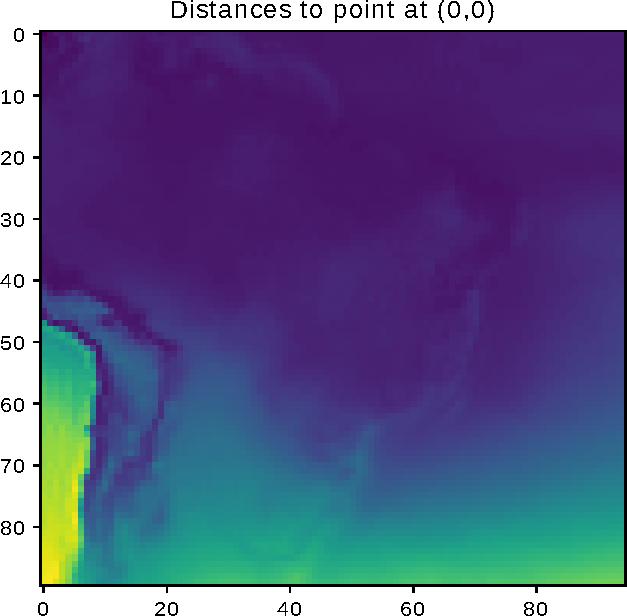
\includegraphics[width=0.45\linewidth]{../Figures/distances_0_0_whole_real_brazil.pdf}
	}
	%no space
	\hfill
	\subfloat{%[DTW distance from the center to the other elements.]{\label{Fig:DTW-DistanceCenter}
		\centering
		
		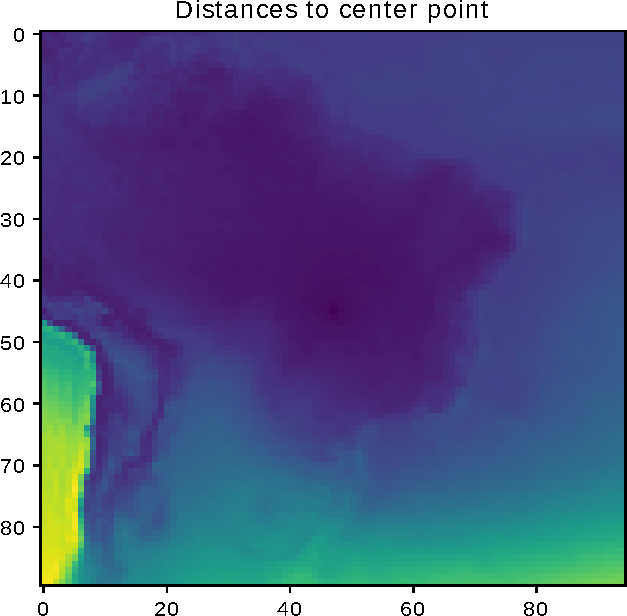
\includegraphics[width=0.45\linewidth]{../Figures/distances_center_whole_real_brazil.pdf}
	}
	\caption{DTW Distance of the time series in the Brazilian region: axes represent spatial indices of the time series, color represents the value of the distance.}
	\label{Fig:DTW-Distance}
\end{figure}

\section{Analyzing the Domain Partitioning Techniques}
\label{Sec:AnalyzeDomainPartitioning}

In this section, we describe the experiments performed to evaluate the strategies adopted for domain partitioning. We consider two partitioning techniques: $k$-medoids based and regular partitioning; the first groups elements of the domain according to the DTW similarity measure, whereas the second is a partitioning technique based on the geometry of the domain (see Section \ref{Sec:DomainPartitioning} for details). In both approaches, we consider representative elements for each group, medoid, and centroid respectively.

%TODO when this hypothesis is evaluated, refer to Section \ref{Sec:AnalyzeDomainPartitioning}
A hypothesis we want to highlight is that using a partitioning technique that considers grouping domain elements based on the similarity of their temporal evolution should produce clusters with lower WSS (see Section \ref{Sec:domain_number_groups}), when compared to creating groups just according to a regular division of the domain geometry. To verify this, we compare the intra-cluster sum of both partitioning techniques for several values of $k$.

Another important aspect of evaluating in $k$-medoids is the choice of the number of partitions ($k$). For this, we use three approaches: elbow method, silhouette index, and the inflection point using a smooth spline (see Section \ref{Sec:domain_number_groups} for a description of these methods).

\subsection{Evaluating Partitioning Quality}
\label{Sec:EvaluatingPP}

In Sections \ref{Sec:DomainPartitioning} and \ref{Sec:domain_number_groups}, we discussed how we could evaluate the robustness of the $k$-medoids clustering by comparing its performance with the regular partitioning when varying the number of groups $k$. Here, we describe the experiments used to assess the quality of the generated partitions and analyze the different techniques used to find useful values for $k$. 

For the two partition techniques, we vary the number of groups from $k=2$ up to $k=150$ with a stride of two. In Table \ref{Table:TotalSumRegularkMedoids}, we show the within-cluster sum of squares (Equation \ref{Eq:WcSS}) for both domain partitioning techniques, with $k$ varying from two to $150$, graphically represented in Figure \ref{Fig:TotalSum-RegularKmedoids}. 

\begin{equation}
    \label{Eq:WcSS}
    WSS = \sum_{i=1}^{k} \sum_{\mathcal{S} \in \mathcal{C}_{i}} d_{DTW} \left(\mathcal{S}, \mathcal{\hat{S}}_{i}\right)^{2}.
\end{equation}

\begin{table}[h]
	\centering
	\tiny
	\begin{tabular}{|c|r|r|c|r|r|c|r|r|}
		\hline
		$k$  & $k$-Medoids & Regular & $k$ & $k$-Medoids & Regular & $k$ & $k$-Medoids & Regular \\ \hline
		2  & 12468.405 & 13190.136 &  52 & 8645.736 & 10032.124 & 102 & 7796.861 &  8855.428 \\
		4  & 11677.377 & 13115.736 &  54 & 8606.070 &  9485.886 & 104 & 7772.689 &  8706.568 \\
		6  & 11218.553 & 12546.427 &  56 & 8566.783 &  9480.166 & 106 & 7752.124 & 12067.876 \\
		8  & 10861.431 & 12517.237 &  58 & 8518.216 & 11466.201 & 108 & 7720.876 &  8404.685 \\
		10 & 10556.589 & 12144.754 &  60 & 8470.036 &  9360.978 & 110 & 7705.371 &  8359.722 \\
		12 & 10320.748 & 11537.237 &  62 & 8432.220 & 11922.456 & 112 & 7676.569 &  8470.927 \\
		14 & 10162.890 & 12038.902 &  64 & 8391.178 &  9238.163 & 114 & 7657.374 &  9012.854 \\
		16 & 10016.352 & 11185.784 &  66 & 8352.620 &  9222.670 & 116 & 7631.154 &  9513.241 \\
		18 &  9874.266 & 11011.460 &  68 & 8315.007 &  9769.658 & 118 & 7612.637 & 11943.777 \\
		20 &  9755.024 & 10864.368 &  70 & 8278.471 &  9148.631 & 120 & 7587.633 &  8276.233 \\
		22 &  9623.499 & 11663.244 &  72 & 8232.783 &  9011.589 & 122 & 7570.840 & 11900.903 \\
		24 &  9539.343 & 10613.759 &  74 & 8203.346 & 11645.734 & 124 & 7547.208 & 10152.428 \\
		26 &  9445.446 & 11741.562 &  76 & 8169.848 &  9864.922 & 126 & 7526.430 &  8218.706 \\
		28 &  9358.812 & 10467.305 &  78 & 8130.028 &  9243.270 & 128 & 7510.721 &  8428.220 \\
		30 &  9279.477 & 10250.783 &  80 & 8101.370 &  8879.863 & 130 & 7485.228 &  8341.508 \\
		32 &  9197.485 & 10305.462 &  82 & 8069.011 & 11478.049 & 132 & 7465.314 &  8149.479 \\
		34 &  9135.674 & 11595.505 &  84 & 8039.939 &  8947.657 & 134 & 7447.742 & 11768.667 \\
		36 &  9083.476 & 10081.895 &  86 & 8014.447 & 11439.713 & 136 & 7431.451 &  8247.420 \\
		38 &  9018.006 & 11685.706 &  88 & 7985.764 &  8719.332 & 138 & 7406.728 &  9136.191 \\
		40 &  8969.207 &  9903.558 &  90 & 7955.133 &  8654.838 & 140 & 7390.761 &  8083.724 \\
		42 &  8902.609 &  9865.422 &  92 & 7922.941 & 10004.969 & 142 & 7366.944 & 11675.846 \\
		44 &  8856.496 &  9990.224 &  94 & 7906.157 & 12251.765 & 144 & 7352.245 &  8126.600 \\
		46 &  8795.638 & 11808.071 &  96 & 7884.088 &  8642.817 & 146 & 7333.966 & 11621.432 \\
		48 &  8740.765 &  9653.982 &  98 & 7855.217 &  8773.346 & 148 & 7311.080 &  9715.298 \\
		50 &  8698.159 &  9605.287 & 100 & 7822.593 &  8525.302 & 150 & 7293.661 &  7932.553 \\ \hline
		
	\end{tabular}
	\caption{Total Within cluster Sum of Squares of $k$-Medoids and Regular Partitioning Techniques for $k = \{2, \ldots, 150\}$.}
	\label{Table:TotalSumRegularkMedoids}
\end{table}


\begin{figure}[h]
	%	\begin{minipage}[b]{0.8\textwidth}
	\centering
	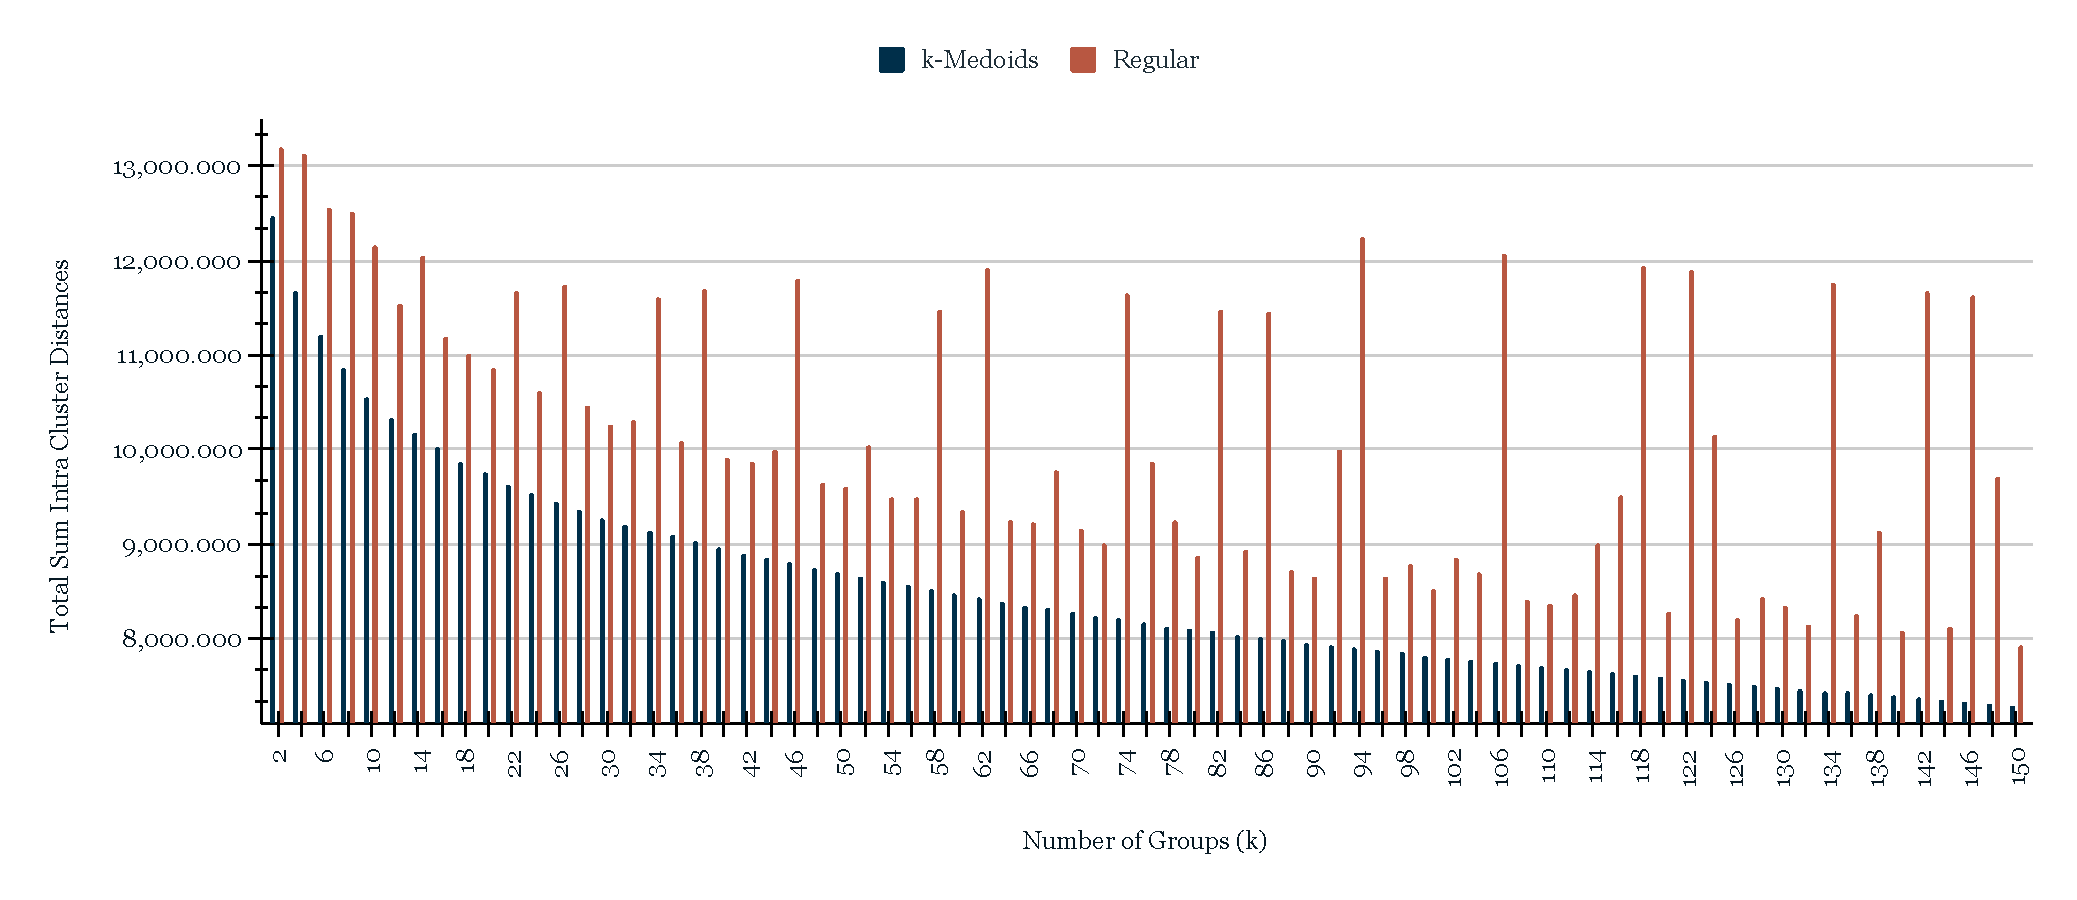
\includegraphics[scale=0.46]{../Figures/Scaled-TotalSum-RegularKmedoids}
	\caption{Total Within cluster Sum of Squares of $k$-Medoids and Regular Partitioning Techniques.}
	\label{Fig:TotalSum-RegularKmedoids}
	%	\end{minipage}
\end{figure}

In the previous figure, it is possible to observe the decreasing behavior of the WSS curve (see Section \ref{Sec:kMedoidsClustering}) for higher values of $k$. In clustering, the goal is to create a cluster from the dataset and create more accurate clusters that can generate insights about the characteristics of the dataset.

\subsection{Selecting $k$}
\label{Sec:Selectk}

% Methods to select k
The $k$-medoids algorithm requires the user to specify $k$, the number of clusters to be generated. When using a clustering technique for high volumes of data and low variability of the data values throughout neighbor points, it is difficult to determine the optimal number of groups. It is particularly important for our problem, where there is low variation in the spatial data distribution of the different time series. In Section \ref{Sec:domain_number_groups}, some methods for determining suitable values for $k$ were discussed. Here, we show the results of applying these methods to our case study as part of Step 1 of our methodology (Section \ref{Sec:DomainPartitioning}) to determine the partitioning schemes that will be used in the later steps.

One common method of choosing the appropriate cluster solution is to compare the Within-Sum-of-Squares (WSS) for a number of cluster solutions. Thus, WSS can be seen as a global measure of error. In general, as the number of clusters increases, the WSS should decrease because clusters are consequently smaller. A plot of the WSS against a series of sequential cluster levels can provide a useful graphical way to choose an appropriate cluster level. An appropriate cluster solution could be defined as the solution at which the reduction in WSS slows dramatically. It produces an ``elbow'' in the plot of WSS against cluster solutions. 

For our dataset, we find an ``elbow'' at the four cluster solution suggesting that solutions greater than four do not substantially impact the total sum of square errors, Figure \ref{Fig:SSE-kMedoids} shows this result. The low number of groups indicated by the elbow method is consistent with the observation (see Figure \ref{Fig:DTW-Distance} and corresponding discussion) that there is a low variability of the temporal data values neighbor points, but which accumulate to produce larger variability throughout the region.

% TODO bigger fonts
\begin{figure}[h]
	%	\begin{minipage}[b]{0.8\textwidth}
	\centering
	\includegraphics[scale=0.5]{../Figures/Elbow-Kmedoids}
	\caption{Application of the Elbow Method, optimal $k=4$ highlighted in red.}
	\label{Fig:SSE-kMedoids}
	%	\end{minipage}
\end{figure}

A second method to consider is the Silhouette Analysis, which explains how close each point in a cluster is to the points in its neighboring clusters. We want to maximize the value of the silhouette score, which would indicate that each sample belongs strongly to its cluster instead of a neighboring cluster.

For the temperature dataset, we performed the silhouette analysis to calculate the score for the range of values of $k$ described in the previous section. The results are in Figure \ref{Fig:Silhouette-kMedoids}, and the maximum score was $0.145$ which corresponds to $k = 8$. 

In general, we obtained low values for the silhouette score throughout the considered range of $k$, indicating that, for high values of $k$, the samples are weakly belonging to their clusters and could also be matched with neighboring clusters. Again, this is an indication that there is low variability throughout neighboring points.

\begin{figure}[h]
	%	\begin{minipage}[b]{0.8\textwidth}
	\centering
	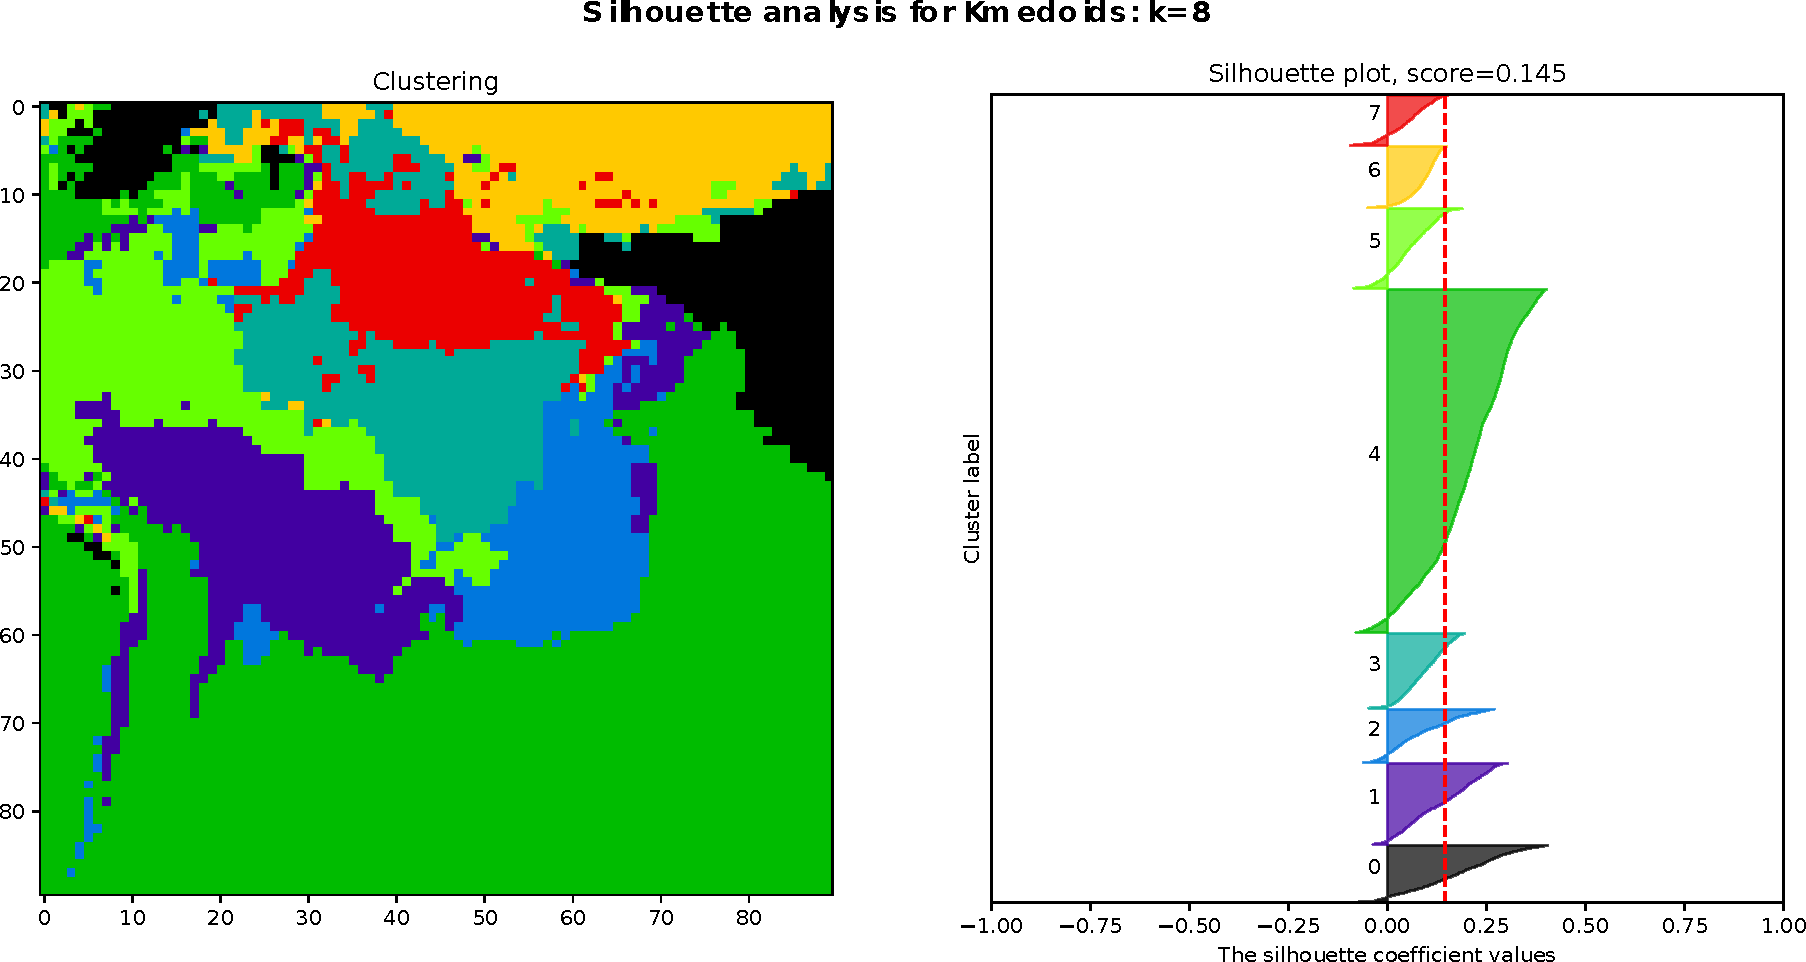
\includegraphics[scale=0.50]{../Figures/silhouette-kmedoids_k8_seed0_lite}
	\caption{Application of the Silhouette Analysis, showing $k=8$ with highest silhouette index.}
	\label{Fig:Silhouette-kMedoids}
	%	\end{minipage}
\end{figure}

An additional method to find the optimal value for $k$, based on the the minimum value for the second derivative, consists of fitting the values of the total sum of intra-cluster distances using a cubic smooth spline. We are interested in finding the point where the curvature of the fitted model is the maximum \cite{Akima1970}. The results for our dataset are shown in Figure \ref{Fig:SmoothSpline-kMedoids}, and the computed value is $k = 66$.

We argue that this method is more appropriate for our dataset, in contrast to the previous two methods, as it highlights the decreasing trend in the intra-cluster cost as $k$ increased. It was possible because the splines smoothed the small variations that were preventing the other methods from finding a higher value for $k$.

\begin{figure}[h]
	%	\begin{minipage}[b]{0.8\textwidth}
	\centering
	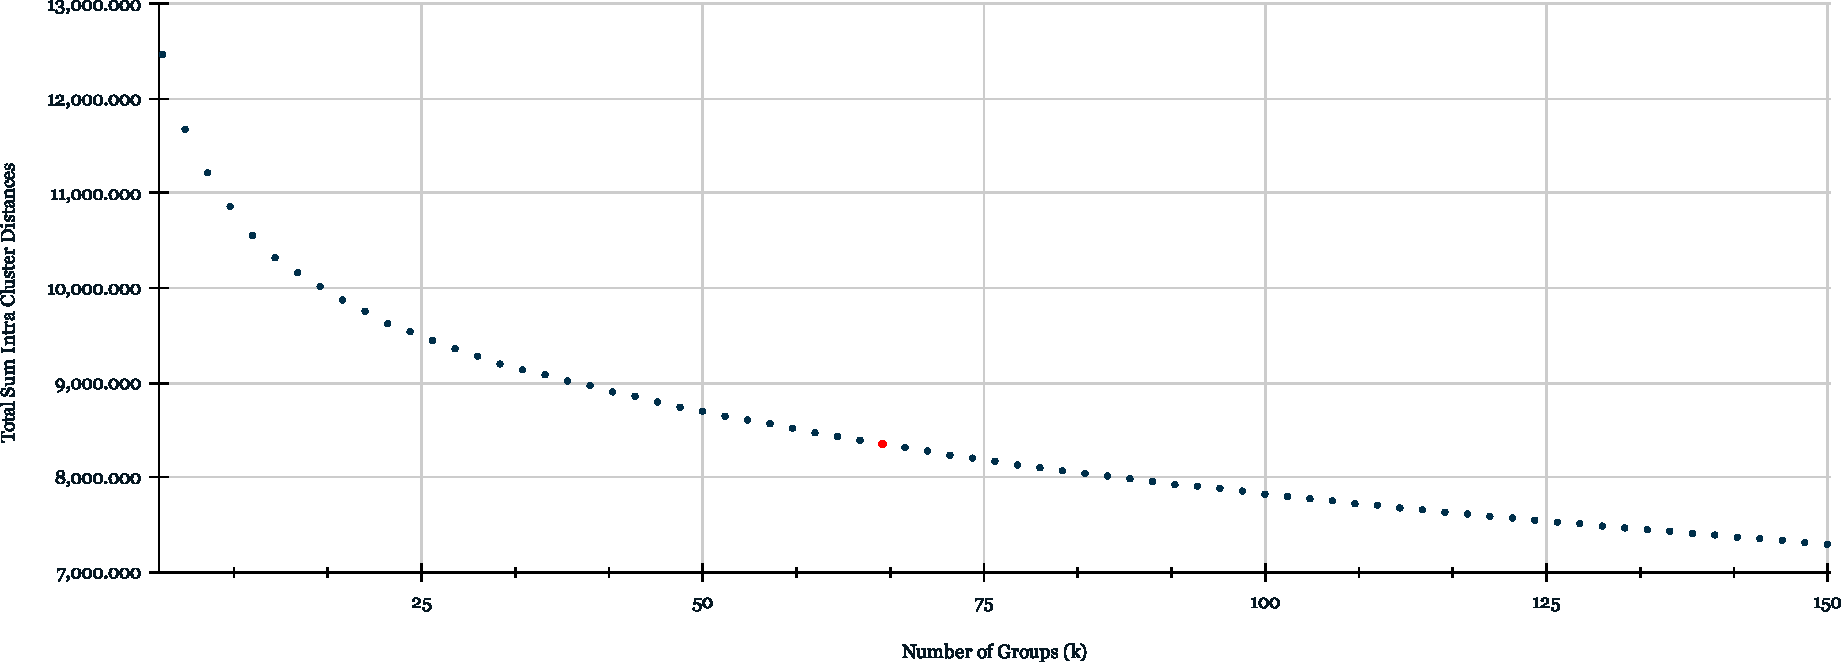
\includegraphics[scale=0.5]{../Figures/SmoothSpline-kMedoids}
	%\caption{Smooth Spline Fitting Method to find the optimal $k$ for the $k$-Medoids Approach.}
	\caption{Application of the Spline Fitting Method, optimal $k=66$ highlighted in red.}
	\label{Fig:SmoothSpline-kMedoids}
	%	\end{minipage}
\end{figure}

We observe that several methods to find an optimal value for $k$ gives us different values. Figure \ref{Fig:OptimalkKMedoids} shows the resulting groups when applying two of these partitioning techniques; the marks indicate the representative points of each group. 
% TODO Argumentar que puede estar pasando
Table \ref{Table:ValidationIndex} summarizes the findings of applying the available methods to find optimal values for $k$.
\begin{table}[h]
	\centering
	\small
	\begin{tabular}{|l|c|}
		\hline
		Method & Optimal $k$ \\ \hline
		Elbow  & 4	\\
		Silhouette & 8	\\
		Smooth Spline for SSE & 66\\ \hline
	\end{tabular}
\caption{Methods to find the optimal value for $k$.}
\label{Table:ValidationIndex}
\end{table}
		
\begin{figure}[htb]
	\centering
	\subfloat{%[DTW distance from the point $(0,0)$ to the other elements.]{\label{Fig:DTW-Distance0}
		\centering
		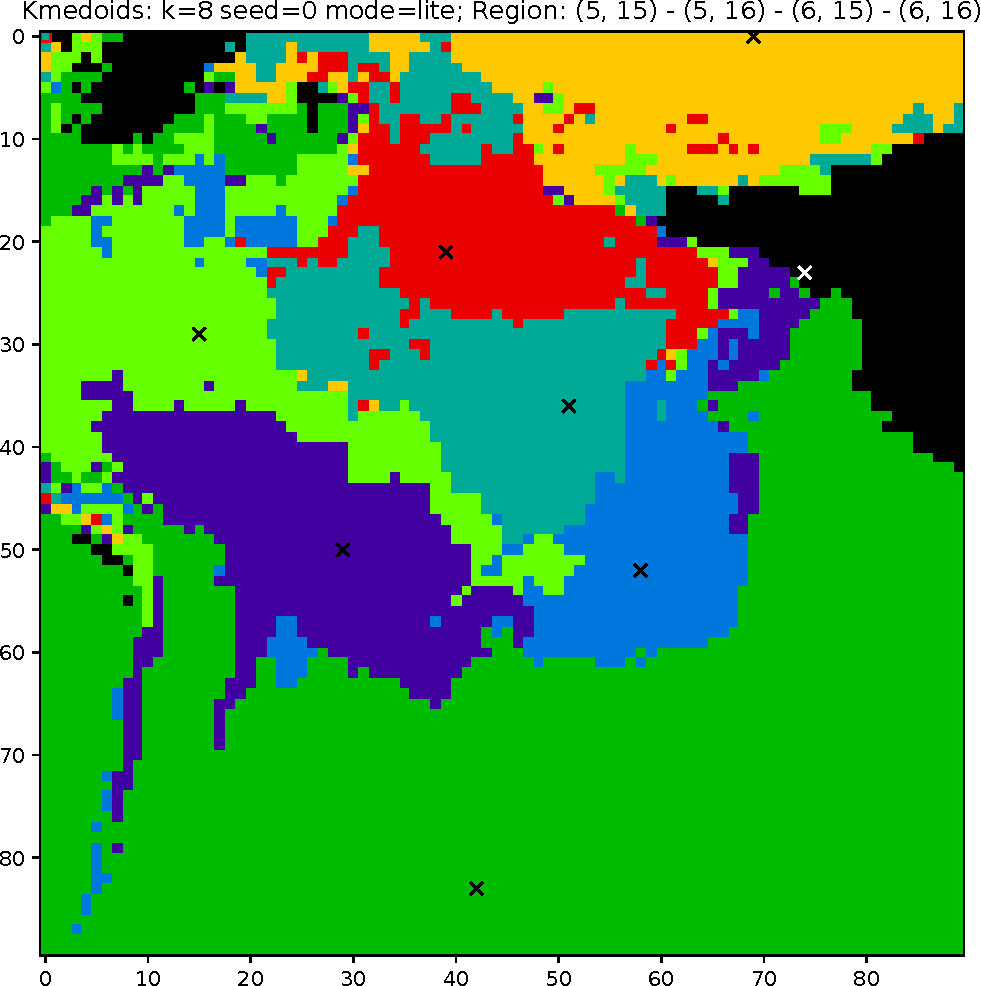
\includegraphics[width=0.45\linewidth]{../Figures/query-kmedoids_k8_seed0_lite__region-0-1-0-1}
	}
	%no space
	\hfill
	\subfloat{%[DTW distance from the center to the other elements.]{\label{Fig:DTW-DistanceCenter}
		\centering
		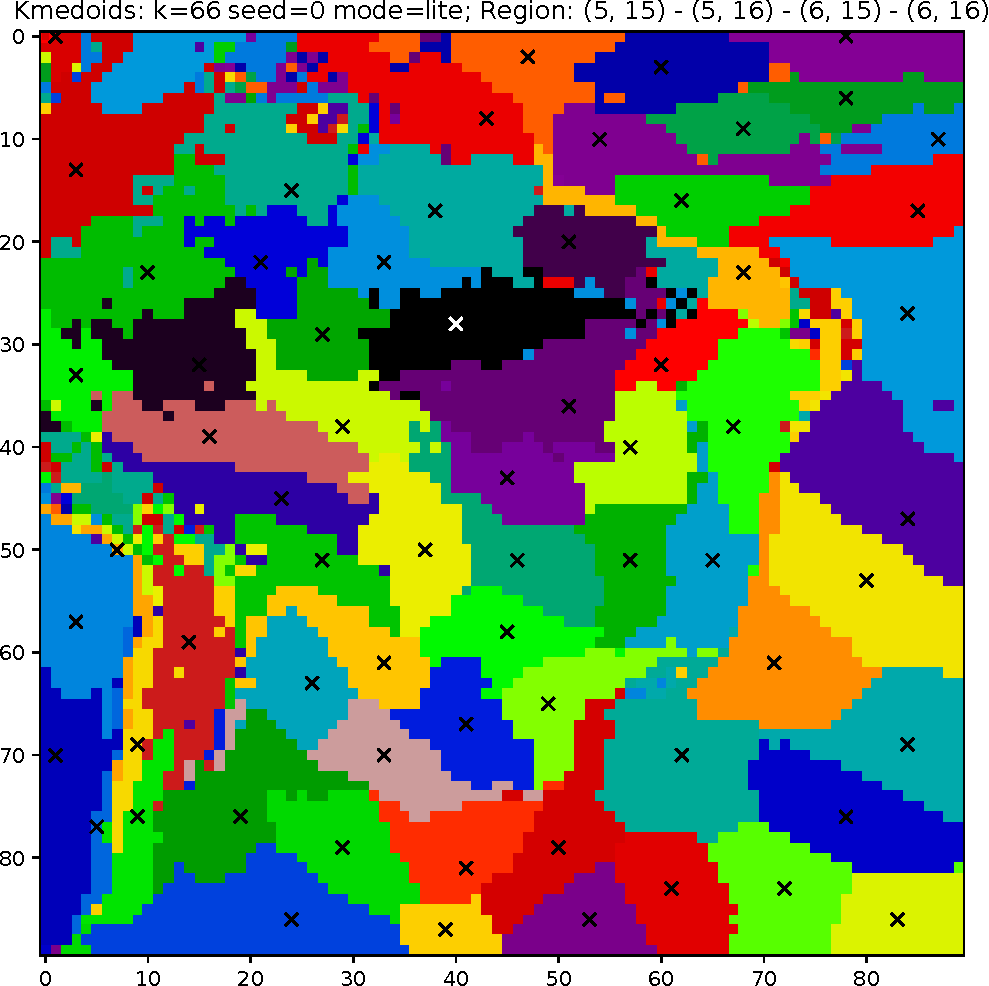
\includegraphics[width=0.45\linewidth]{../Figures/query-kmedoids_k66_seed0_lite__region-0-1-0-1}
	}
	
	\caption{Groups obtained with $k$-Medoids using $k=8$ (left) and $k=66$ (right). Corresponding medoids are marked with a `$\times$'.}
	\label{Fig:OptimalkKMedoids}
\end{figure}	

\subsection{Discussion on Domain Partitioning}
\label{Sec:DomainPartitioningDiscussion}

% Justification and Summarization
Spatial-temporal data are heterogeneous and autocorrelated. Consequently, the data are consistent and smoothly variable \cite{Cressie2011}. The division of the domain into $k$ parts by a method that considers the similarity in the temporal evolution of its elements is superior to a method that does not consider any similarity. Furthermore, there is more than one $k$ that, based on temporal similarity, expresses better different regions of the domain.

The evaluation of this part of the methodology allowed us to establish the $k$-medoids algorithm as a significantly superior partitioning solution, compared to the naive approach of a regular partitioning used as a baseline. It was demonstrated even when increasing the number of groups. While both partitioning algorithms exhibit a decreasing trend in the sum of intra-cluster distances (partitioning cost), the cost of the $k$-medoids algorithm was consistently smaller than the baseline. Also, the trend was monotonous for $k$-medoids, while it showed variability for the regular partitioning (the latter variability can be explained by the arithmetic of dividing the region in equal rectangles). 

The monotonous trend of $k$-medoids allowed for calculating the inflection point, which effectively calculated a high value for $k$ to represent a suitable partitioning scheme ($k = 66$). This value gives us a reasonable number of representatives to use in the next phases of the methodology. Also, since we applied two other validation methods for selecting $k$ that produced two other domain partitioning schemes, we can also consider these groups and their representatives when evaluating a model composition. 

% FIXME add comment on k = 132, how was it chosen? Also why not using k=4 obtained with the elbow method.

% DBSCAN-Not included in the final version to avoid confusion or off-topic discussions.
%In addition to $k$-Medoids, we also explored DBSCAN, another clustering method that can also use DTW as the similarity measure. DBSCAN is a procedure to find `optimal' number of groups based on the spatial density of the data, and uses two parameters: the maximum ray to agglomerate points and the minimum number of elements per group. Its disadvantage is that being an algorithm that only finds convex groups, if the elements are not similar they are considered outliers. When DBSCAN was applied to our dataset, it would either find only two groups containing most of the data points, or few groups that failed to contain most of the points, because DBSCAN would mark other points as outliers. After this exploration of DBSCAN, further analysis with it was discontinued.

In the following section, we describe the process to generate predictive models on the representative elements and the experiments to evaluate their predictive quality.

\section{Predictive Quality of Models on Representatives}
\label{Sec:AnalyzePredictorRepresentatives}

This section performs extensive experiments to evaluate the predictive quality of models trained on representative elements (medoid or centroid) for different domain partitioning sizes. One reason to adopt this approach is to accelerate the computationally intensive process involved when considering training models for every element in the domain. The evaluation of their efficiency is also a time consuming process \cite{Hyndman2018}.

% Predictor ARIMA
In Step Two of our proposed methodology (Section \ref{Sec:ModelRepresentatives}), we generate an ARIMA model for each representative obtained from the domain partitioning. Once an appropriate time series model has been fit, it may generate forecasts of future observations. To evaluate the forecast accuracy of these models, we consider the following experiments:

\begin{enumerate}
    \item In-sample and forecast errors: we look at a single model and describe how we evaluate the forecast of future predictions by comparing with the actual observational values, using the sMAPE measure.
    \item Forecast errors for a Domain Partitioning: we analyze the forecast errors when a predictive model trained in a representative is used to predict the time series of elements of its corresponding group; this is done for many domain partitioning sizes.
    \item Forecast errors in a Model Composition: we look at different ways to select the representative used to create the forecast of each element and aggregate errors using MSE. It is explored in detail in the next section.
\end{enumerate}

The calculation of the in-sample error corresponds to the `Evaluate In-Sample Error' item presented in Step Two of the methodology (Figure \ref{Fig:OverviewMethodology}). The additional experiments listed above (not included in Chapter \ref{Chapter:Methodology}) are not required to produce a model composition capable of processing predictive queries; but will allow us to assess the accuracy of the models and better justify aspects of the methodology. This analysis can be described as creating an additional process after Step Two (see Figure \ref{Fig:MethodologyExperiments}). 

\begin{figure}[h!]
	\centering
	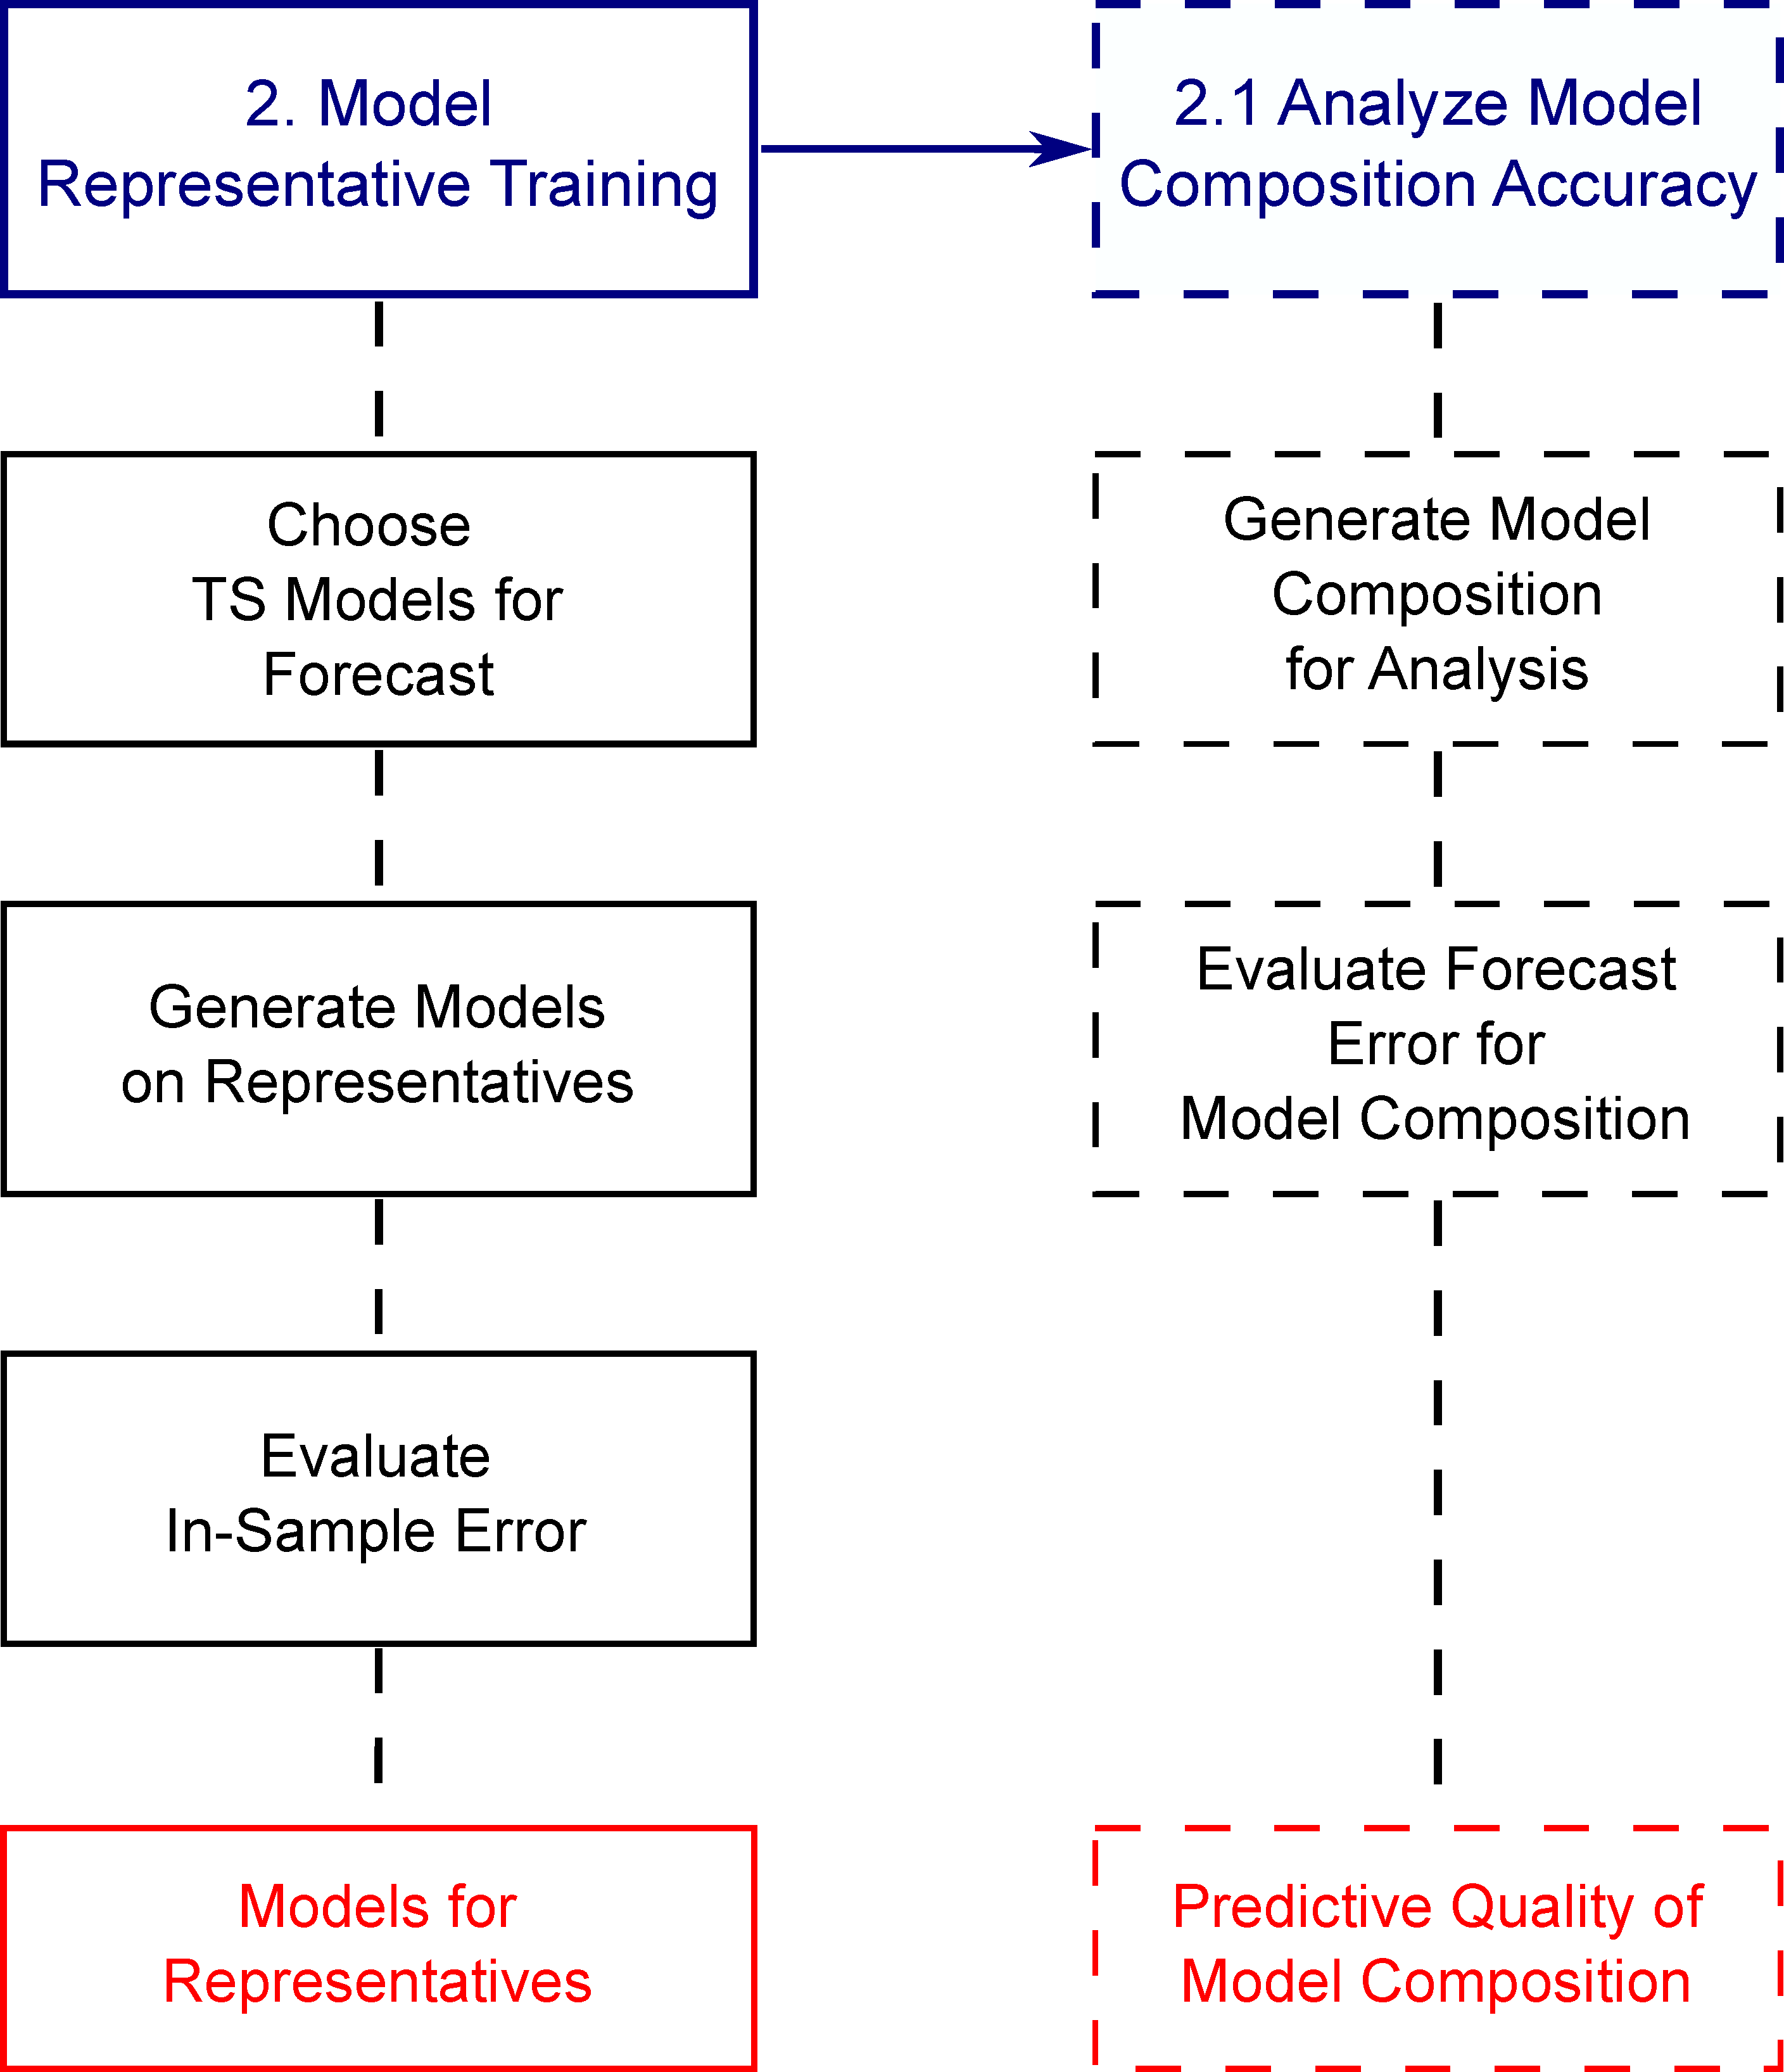
\includegraphics[scale=0.18]{Figures/Experiments_Methodology_Step2_Step2.1_corrections}
	\caption{Predictive Quality Analysis for Model Composition.}
	\label{Fig:MethodologyExperiments}
\end{figure}

We introduce an additional concept to support the analysis, the prediction interval \ref{Sec:ErrorTSA}. It is similar to a confidence interval, an estimate of the range of likely values that are not yet known but are going to be observed at some point in the future \cite{Chatfield2001}. A prediction interval needs to consider uncertainty in the model, uncertain estimates of the parameters in a model (i.e., the confidence intervals for those parameters), and the individual randomness associated with the predicted particular points.

\subsection{Obtaining In-sample and Forecast Errors}
\label{sec:InSampleForecastErrors}

Let's consider a particular representative $\mathcal{S}^{*} \in \mathbf{R}$ and its associated temperature series $\lbrace s_t \rbrace$. In order to train and test the predictive accuracy of an ARIMA model, we split the time series as shown in Figure \ref{Fig:TimeSplit}. Recalling the preparation of the dataset described in Section \ref{sec:DatasetPreparation}, we work with 365 values for each representative point, denoted by the series:

\begin{equation}
    \{s_{t} \} = \{s_{0}, s_{1}, \ldots s_{364} \}
\end{equation}

\begin{figure}[h!]
	\centering
	\includegraphics[scale=0.38]{../Figures/ModelRegion_ModelTS}
	\caption{Time units split for training and test datasets.}
	\label{Fig:TimeSplit}
\end{figure}

To evaluate an ARIMA model $g_{\mathcal{S}^{*}}$ and its predictive power, the series is split into three parts. The first part $s^{tr}_t = \lbrace s_0, s_1, \ldots s_{349} \rbrace$ is used for training the model, %($s^t_r[0:349]$ as an example in Figure \ref{Fig:Time-SeriesSplit})
here we determine the tuple $(p_{\mathcal{S}^{*}}, d_{\mathcal{S}^{*}}, q_{\mathcal{S}^{*}})$ that determines the model $g_{\mathcal{S}^{*}}$. Then, we take the next $t_p$ data points ($t_p = 8$ in our example) to create the test series $s^{ts}_t = \lbrace s_{349}, \ldots s_{356} \rbrace$.
%$s^v_t[349:357]$.

The purpose of this split is to obtain the in-sample error ${E^*}$ of the model: this is achieved by using the model $g_{\mathcal{S}^{*}}$ to predict $t_p$ steps and then calculating an associated error using one of the error expressions presented in Section \ref{Sec:ModelRepresentatives}.

\begin{figure}[h!]
	\centering
	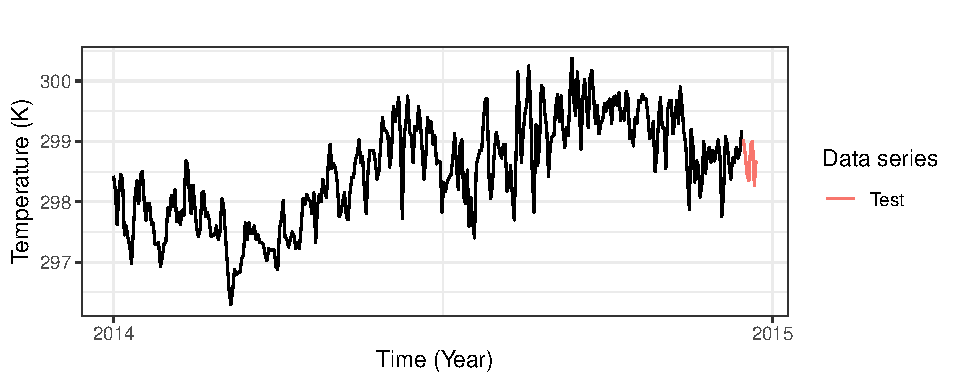
\includegraphics[scale=1]{../Figures/medoid_test_training}
	\caption{Dataset Split for a Time Series Representative ($s^{tr}_t$ in black, $s^{ts}_t$ in pink).}
	\label{Fig:Time-SeriesSplit}
\end{figure}

Then, the model is retrained using the same $(p_{\mathcal{S}^{*}}, d_{\mathcal{S}^{*}}, q_{\mathcal{S}^{*}})$ model parameters found with $s^{tr}_t$, but now using a longer series $\lbrace s_0, s_1, \ldots s_{356} \rbrace$ (previous training series now extended with the test series). In order to evaluate the model's predictive power, we use it to forecast $t_f$ steps into the future ($t_f = 8$ in our example) that the model has not seen. However, since the subset $\lbrace s_{357}, \ldots s_{364} \rbrace$ is available from the dataset, it is possible to evaluate the forecast error. As a result of this approach, we can perform forecast error analysis on different representatives from different domain partitioning schemes.
%The error analysis described can also be applied to the $k$NN predictive model (baseline).

In order to show this approach in action, we present Figures \ref{Fig:ModelFinalToForecast} and \ref{Fig:ForecastElement1}. In Figure \ref{Fig:ModelFinalToForecast}, we show the ARIMA model with parameters $(3,1,1)$ for a medoid in a domain partitioning ($k=8$). Represented with a blue line, we have the forecast values for $t_{f} = 8$, while the prediction intervals with $95\%$ and $80\%$ levels are shown in blue and light blue shades, respectively. The values fitted by the model are also shown in pink, on top of the original time series for the retrained model in black.

Given that the prediction intervals are available and the future values ($t_f = 8$) of the temporal series in the domain are known, it is possible to determine whether or not the future values of the series are contained within the prediction intervals, in this way we can qualify the effectiveness of the predictive model in a representative. It is shown in Figure \ref{Fig:ForecastElement1}: in addition to showing the time series of the representative in black and the prediction intervals calculated for the corresponding predictive model, we show the actual time series of a different element in the domain (attributed by the representative) in pink. We can see in this case that all the future values are contained within the prediction interval with $80\%$ level, while most of the time series is also contained inside the $95\%$ level. It gives us a reasonable level of confidence that the predictive model is functioning as a predictor for this element in the interval considered.

\begin{figure}[!ht]
	\centering
	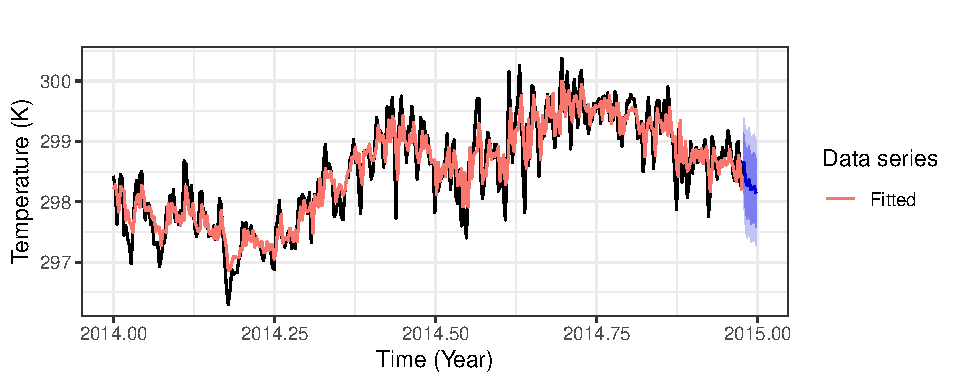
\includegraphics[scale=1]{../Figures/medoid_forecast_fitted}
	\caption{Example of a fitted ARIMA forecast at a representative with out-of-sample prediction intervals.}
	% Change caption.
	\label{Fig:ModelFinalToForecast}
\end{figure}

% Add the forecast <
\begin{figure}[!ht]
	\centering
	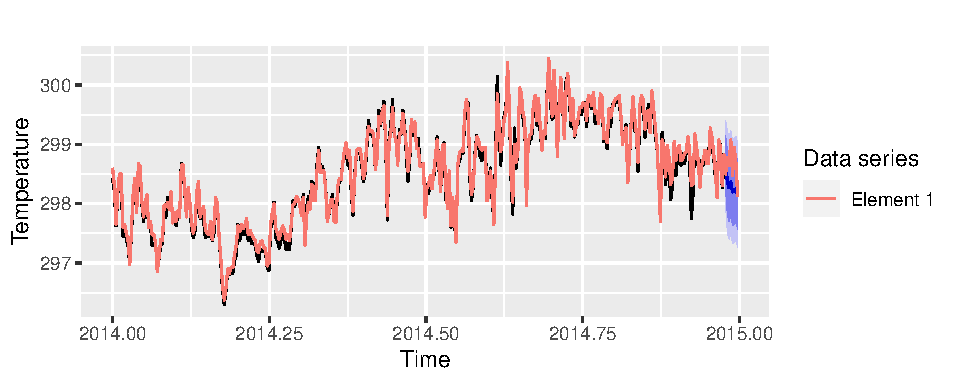
\includegraphics[scale=1]{../Figures/forecast_element1}
	\caption{Example of a time series (in pink) and its prediction, using the ARIMA model at its representative from Figure \ref{Fig:ModelFinalToForecast}.}
	% Change caption.
	\label{Fig:ForecastElement1}
\end{figure}

For ARIMA models, we use the sMAPE measure to describe how well a model fits a given sample of data. This goodness-of-fit approach uses the residuals of model fitting and may not reflect the capability of the forecasting technique to predict future observations \cite{Montgomery2015} successfully. The end-user of a predictive system is concerned about the accuracy of future forecasts, not model goodness-of-fit, so it is important to evaluate this aspect. Sometimes forecast accuracy is called `out-of-sample' forecast error to distinguish it from the residuals. Next, we analyze forecast errors of the models on the representatives when used to predict other elements.

\subsection{Forecast Error of Models on Representatives}
\label{Sec:AnalyzeForecastErrors}

The previous section described the process of calculating a multi-step prediction for the future values of a time series, using a predictive model trained on the representative. Given that the out-of-sample interval of length $t_f$ is known from the dataset, we can then present results on evaluating the corresponding forecast error. The analysis will be performed for both $k$-medoids and regular partitioning.

We begin by analyzing the forecast errors when using $k$-Medoids as partitioning scheme (which yields the medoids as representatives) and the auto ARIMA procedure as the predictive model. In the case of a $k=8$, we have eight groups with the number of elements in average $1012.5 \pm 1003.807$, representing between the $6.2\%$ and $43\%$ of the domain. It means that there are eight possible predictive models that we can use to make predictions for any element in the domain.

By considering a larger value for the number $k=66$, we create more groups and, therefore, more representatives that generalize better the elements in its group. The partitioning domain result is grouped with an average of $122.727 \pm 49.974$, representing between the $0.2\%$ and $3.4\%$ of the domain. For $k=132$, we obtain groups with elements in average $61.363 \pm 17.913$, representing between the $0.2\%$ and $1.2\%$ of the domain.

% TODO single "Figure" with subfigures?
To qualify the predictive power of the representative predictor forecast error for each element of its group, we compute the sMAPE error of the prediction from the representative model for each element. We perform an exploratory analysis using scatter plots diagrams that aggregate the sMAPE results, shown in Figures \ref{Fig:DTWsMAPE_k8_c0}-\ref{Fig:DTWsMAPE_k132_c15}. The diagrams show the DTW distance of each element to its medoid in the $x$-axis and the sMAPE forecast errors in the $y$-axis. For different domain partitioning schemes ($k=\{8, 66, 132\}$), we show in the left column the `best' representatives, for which the maximum forecast error is the lowest, and on the right column are the representatives for which the maximum forecast error is the highest.
% TODO Explicar mejor lo que obtenemos.

% k=8
\begin{figure}[!htbp]
  \centering
  \begin{minipage}[b]{0.45\textwidth}
    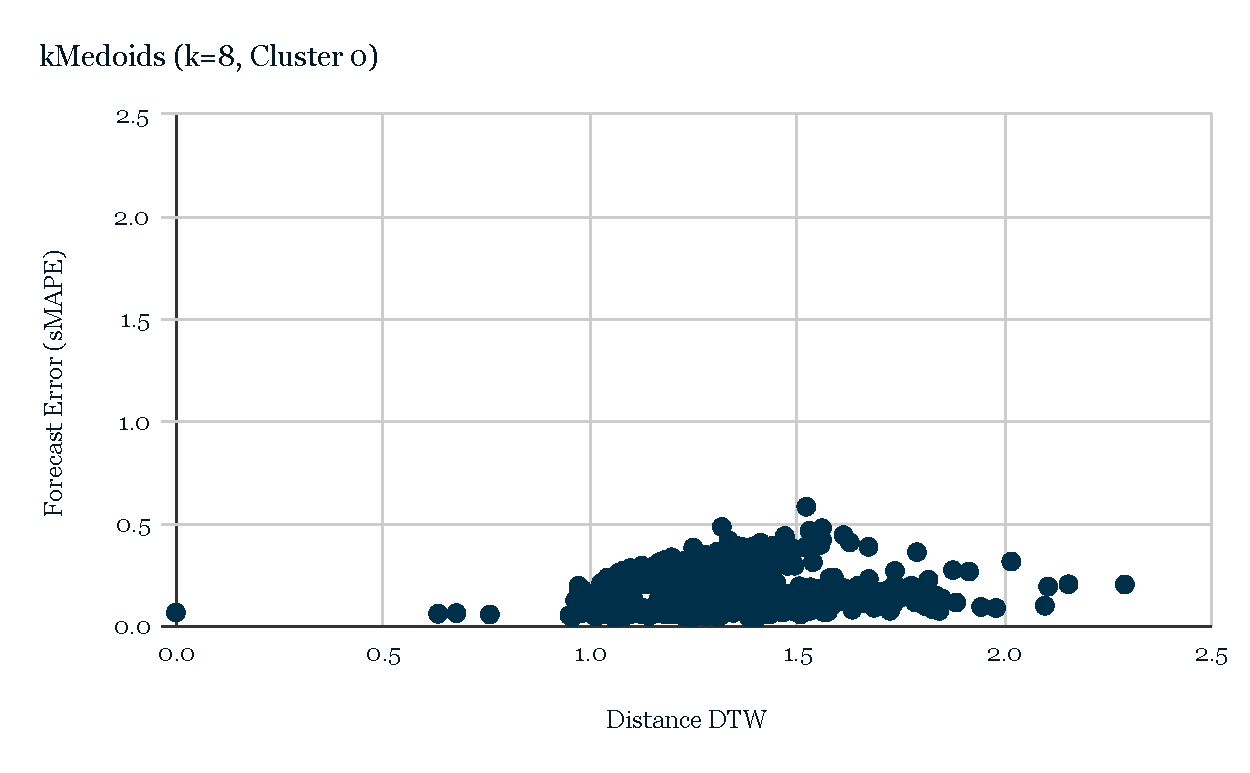
\includegraphics[width=\textwidth]{../Figures/distDTW_ForecastError_k8_c0}
    \caption{Forecast Error with $t_{f}=8$ (for $n=574$ elements) averaged $0.159 \pm 0.073$.}
    \label{Fig:DTWsMAPE_k8_c0}
  \end{minipage}
  \hfill
  \begin{minipage}[b]{0.45\textwidth}
    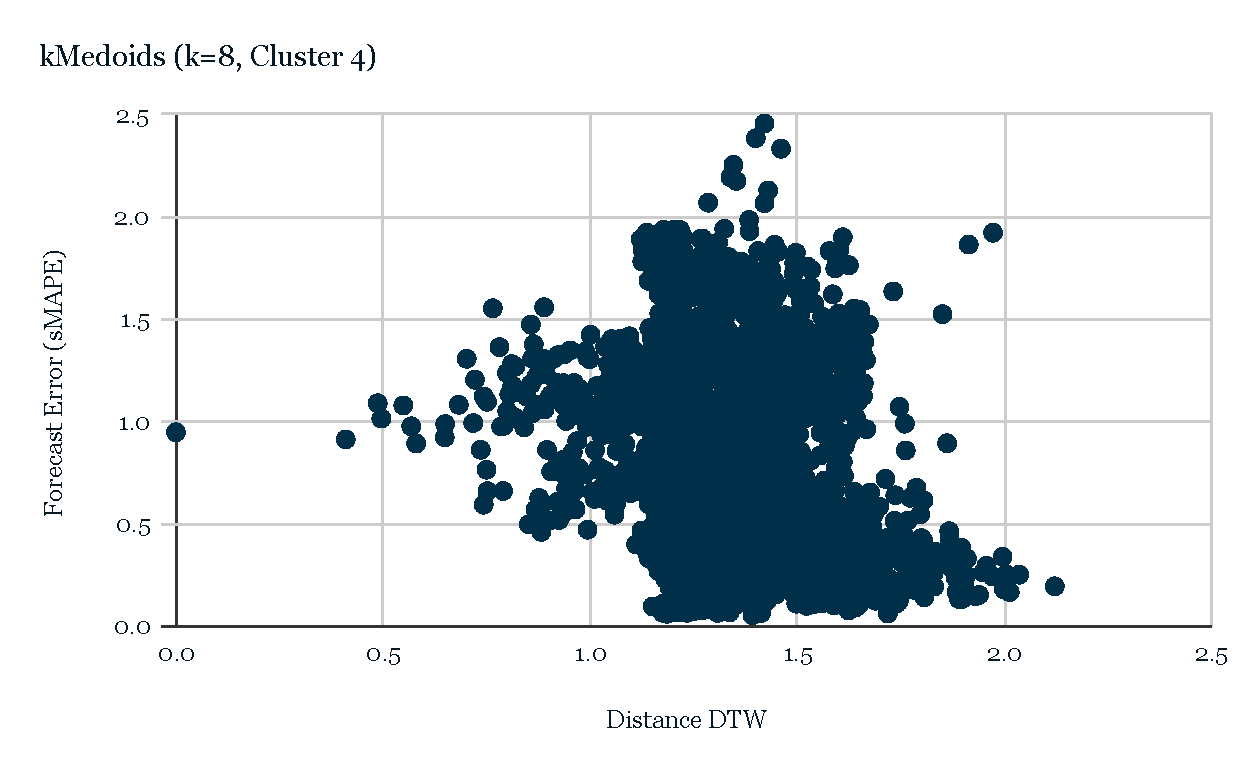
\includegraphics[width=\textwidth]{../Figures/distDTW_ForecastError_k8_c4}
    \caption{Forecast Error with $t_{f}=8$ (for $n=3479$ elements) averaged $0.718 \pm 0.347$.}
    \label{Fig:DTWsMAPE_k8_c4}
  \end{minipage}
% \end{figure}

% k=66
% \begin{figure}[!tbp]
  \centering
  \begin{minipage}[b]{0.45\textwidth}
    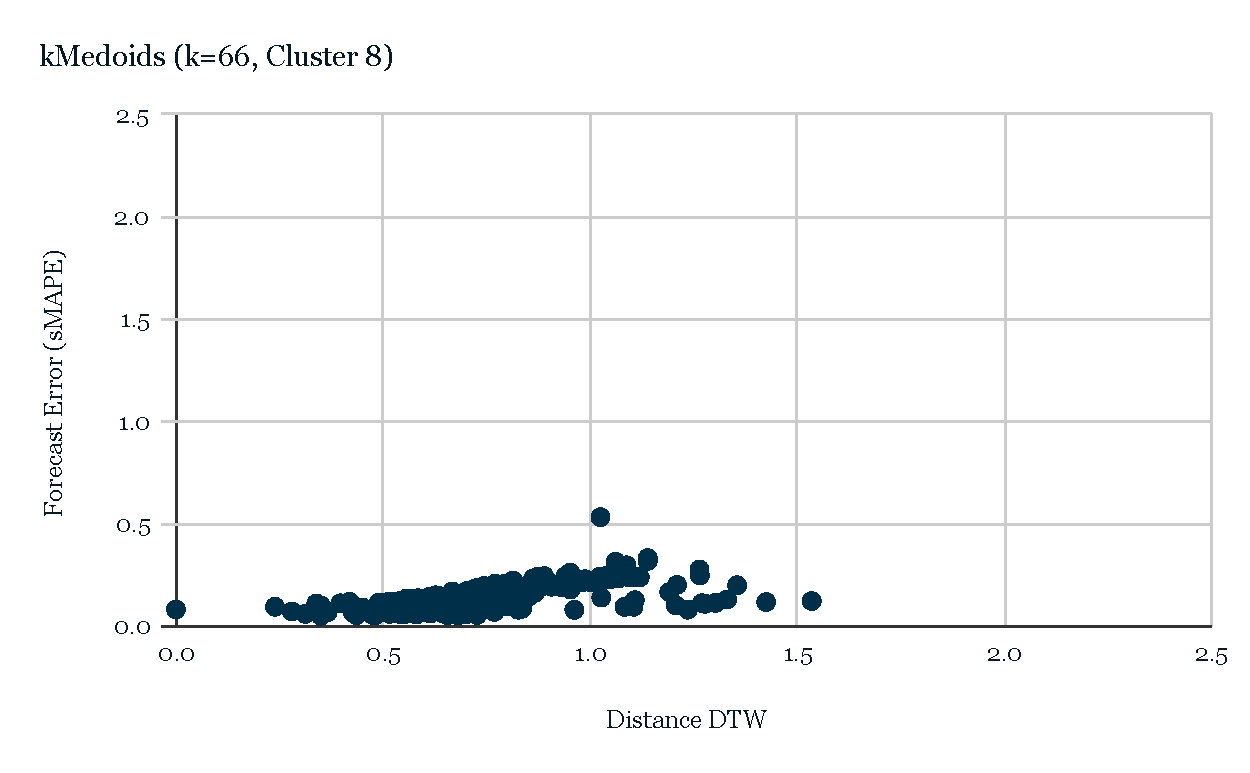
\includegraphics[width=\textwidth]{../Figures/distDTW_ForecastError_k66_c8}
    \caption{Forecast Error with $t_{f}=8$ (for $n=215$ elements) averaged $0.142 \pm 0.054$.}
    \label{Fig:DTWsMAPE_k66_c8}
  \end{minipage}
  \hfill
  \begin{minipage}[b]{0.45\textwidth}
    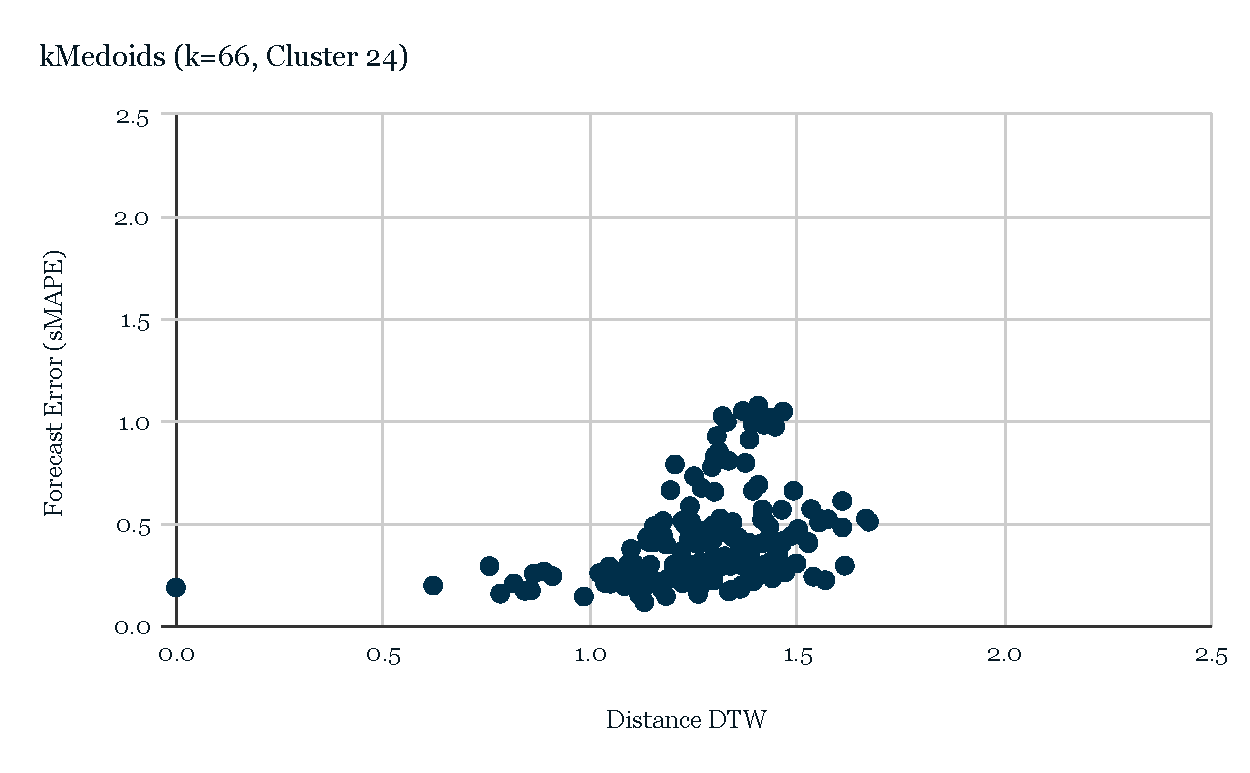
\includegraphics[width=\textwidth]{../Figures/distDTW_ForecastError_k66_c24}
    \caption{Forecast Error with $t_{f}=8$ (for $n=182$ elements) averaged $0.400 \pm 0.172$.}
    \label{Fig:DTWsMAPE_k66_c24}
  \end{minipage}
%\end{figure}

% k=132
%\begin{figure}[!tbp]
  \centering
  \begin{minipage}[b]{0.45\textwidth}
    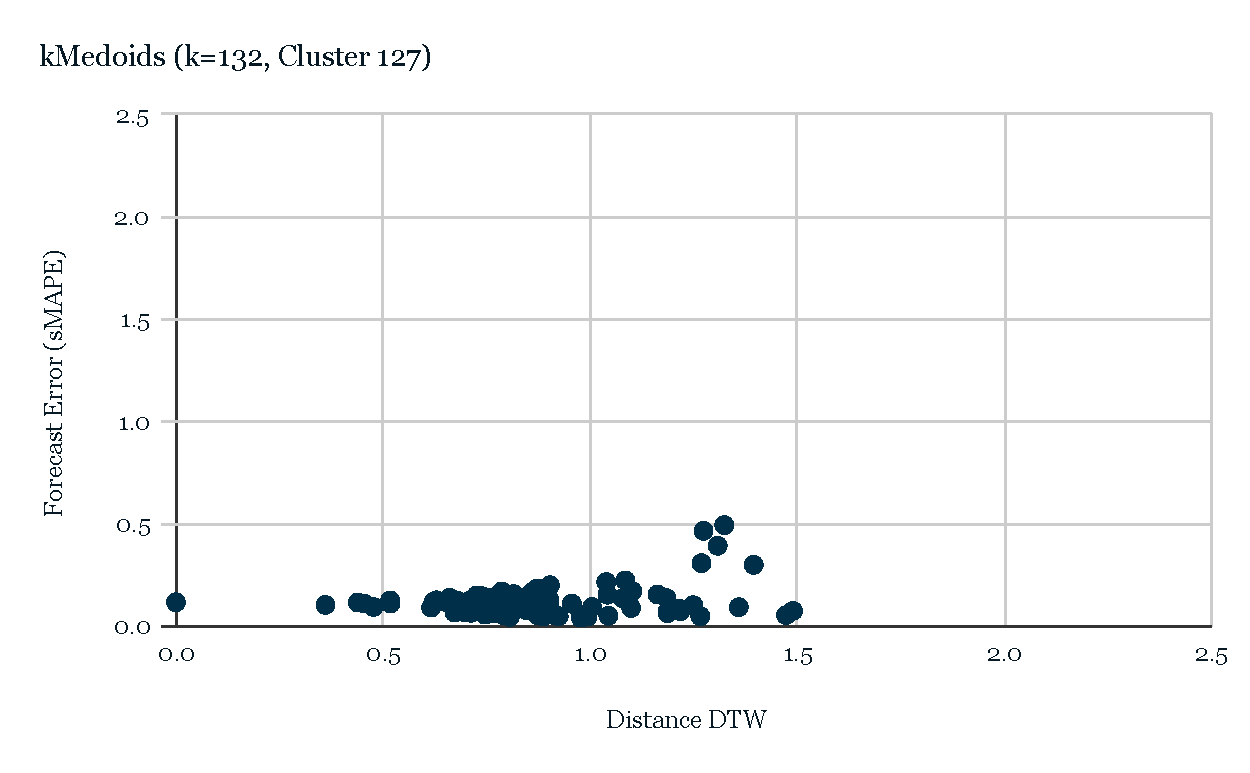
\includegraphics[width=\textwidth]{../Figures/distDTW_ForecastError_k132_c127}
    \caption{Forecast Error with $t_{f}=8$ (for $n=121$ elements) averaged $0.117 \pm 0.042$.}
    \label{Fig:DTWsMAPE_k132_c127}
  \end{minipage}
  \hfill
  \begin{minipage}[b]{0.45\textwidth}
    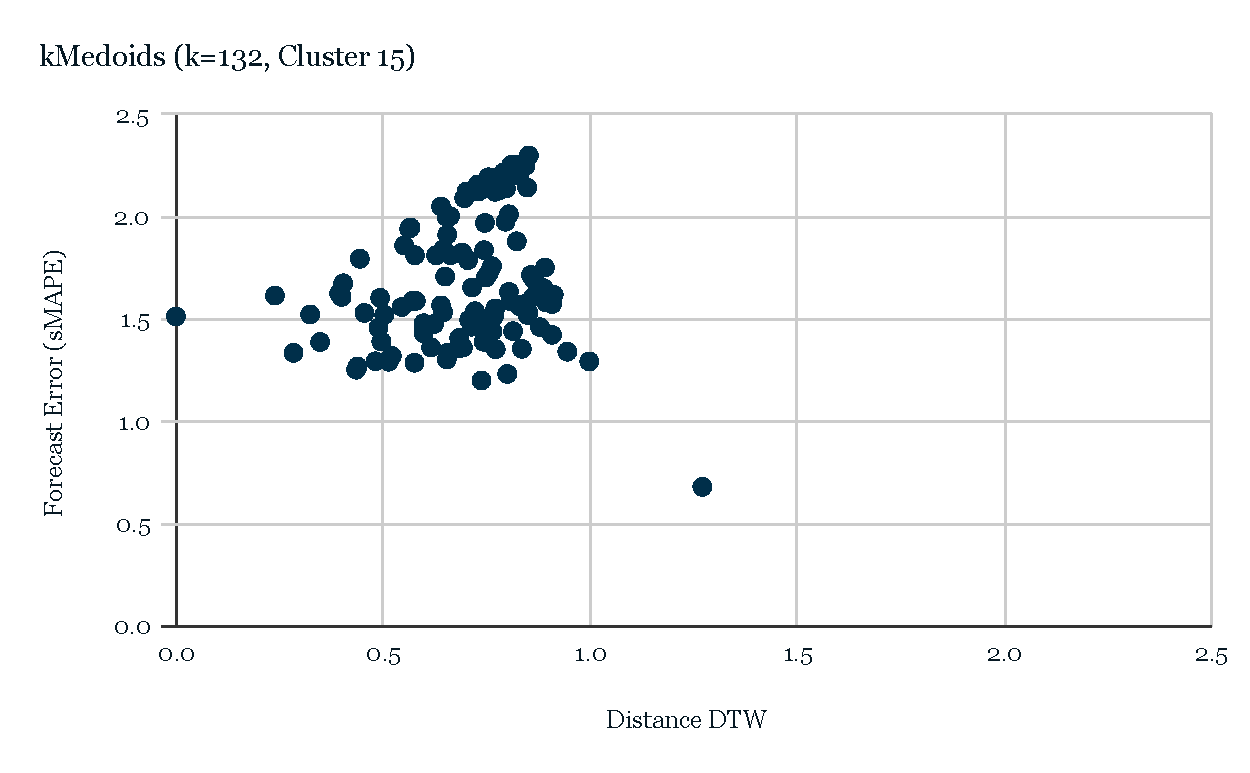
\includegraphics[width=\textwidth]{../Figures/distDTW_ForecastError_k132_c15}
    \caption{Forecast Error with $t_{f}=8$ (for $n=119$ elements) averaged $1.690 \pm 0.271$.}
    \label{Fig:DTWsMAPE_k132_c15}
  \end{minipage}
\end{figure}

\newpage
We can observe that, for each representative considered, there is not a clear correlation between the values of the DTW distance and the forecast error. When we considered all the available data from all the representatives (the axes in all figures was standardized to see this more easily), we can see is that, as $k$ increases, there is a tendency to obtain groups with more similarity between their elements (lower DTW distance) and also the forecast error tends to be lower. It means that each representative from a partitioning scheme with more groups is generally able to make more accurate predictions of the elements in its group.

However, an important observation here is that lower values of $k$ (8, 66) can produce some representatives that offer better predictions than, for example, the `worst' (highest forecast error) representatives of the partitioning scheme with $k=132$. This result justifies the inclusion of the classifier in our methodology because there is potential for improved accuracy when considering representatives from multiple partitioning schemes.

A similar analysis with scatter plots is performed with the regular partitioning domain and shown in Figure \ref{Fig:DTWsMAPE_r8_g5}-\ref{Fig:DTWsMAPE_r132_c121}. In this case, we can observe that the points are more dispersed and with larger variations in the forecast errors, especially for $k = 66$ and $k = 132$. This result strengthens the advantage of grouping the domain under the similarity based on the shape of its elements rather than by a mere division based on the geometry of the domain.

% k=8
\begin{figure}[!htbp]
  \centering
  \begin{minipage}[b]{0.45\textwidth}
    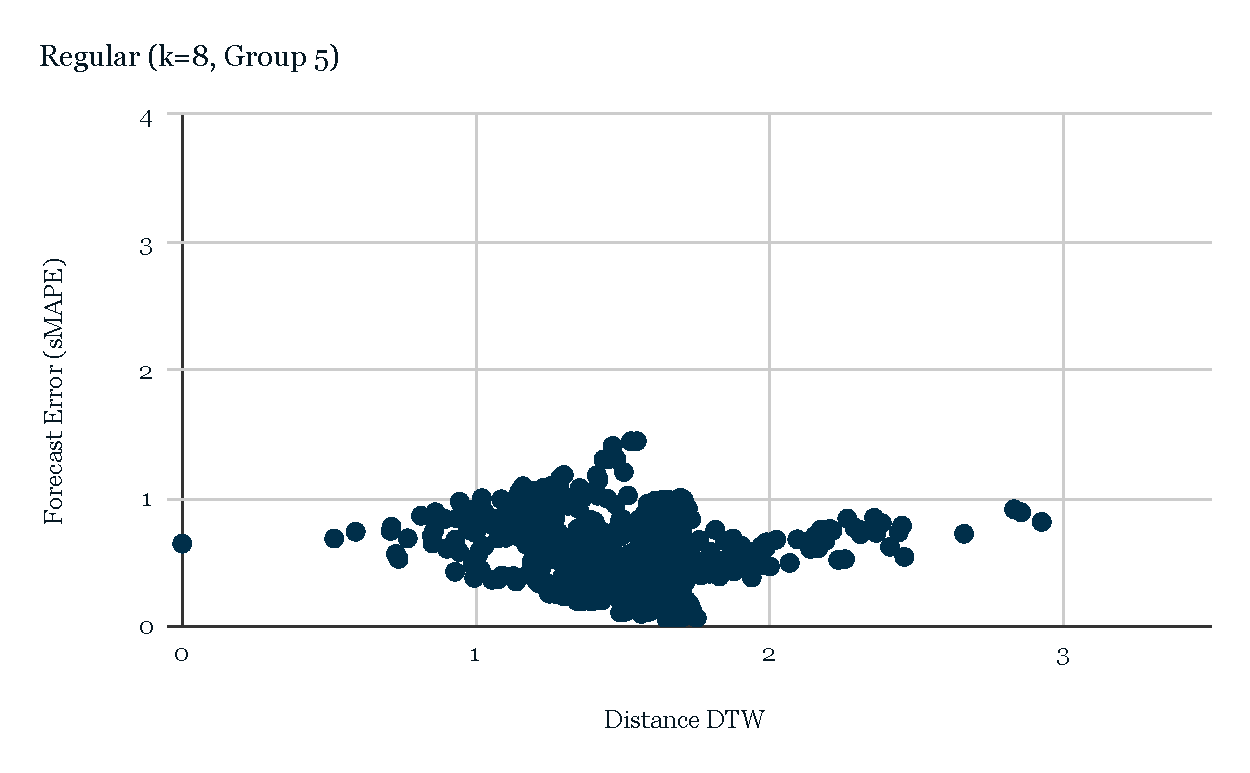
\includegraphics[width=\textwidth]{../Figures/distDTW_ForecastError_r8_c5}
    \caption{Forecast Error with $t_{f}=8$ (for $n=990$ elements) averaged $0.551 \pm 0.220$.}
    \label{Fig:DTWsMAPE_r8_g5}
  \end{minipage}
  \hfill
  \begin{minipage}[b]{0.45\textwidth}
    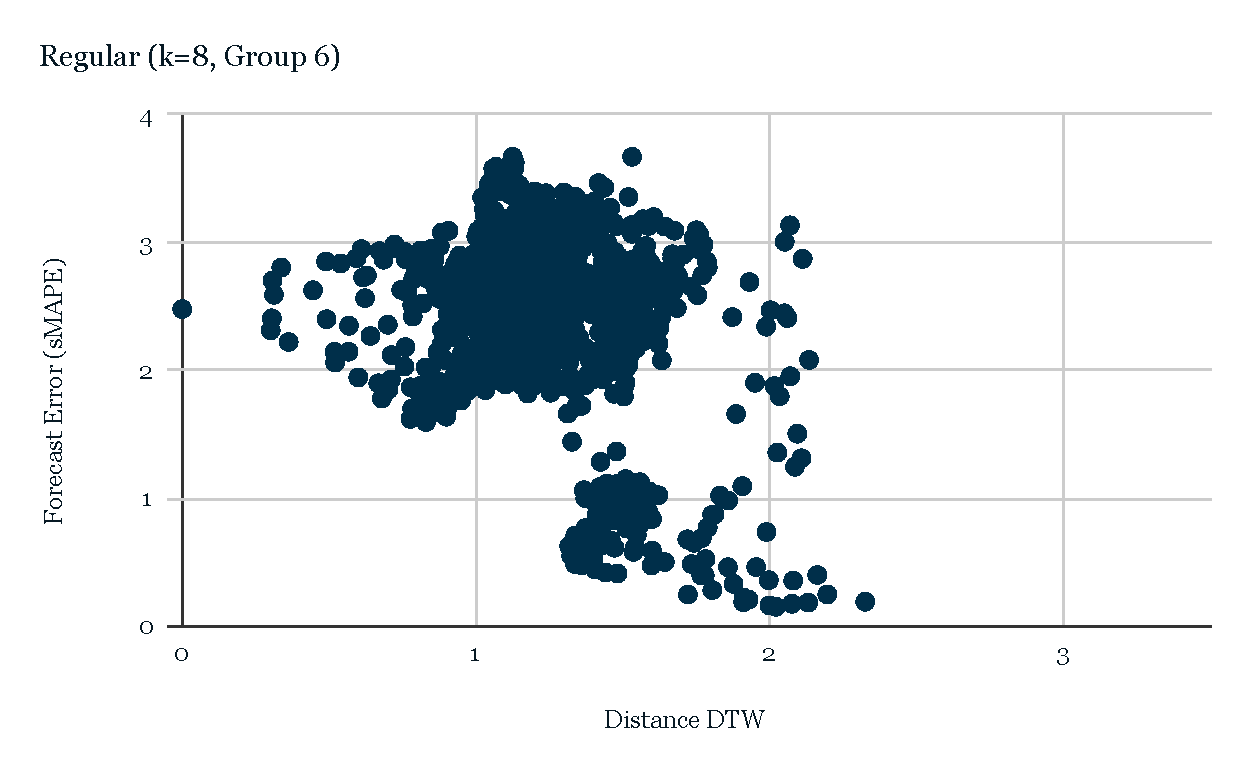
\includegraphics[width=\textwidth]{../Figures/distDTW_ForecastError_r8_c6}
    \caption{Forecast Error with $t_{f}=8$ (for $n=1080$ elements) averaged $2.330 \pm 0.584$.}
    \label{Fig:DTWsMAPE_r8_g64}
  \end{minipage}
\end{figure}

% k=66
\begin{figure}[!tbp]
  \centering
  \begin{minipage}[b]{0.45\textwidth}
    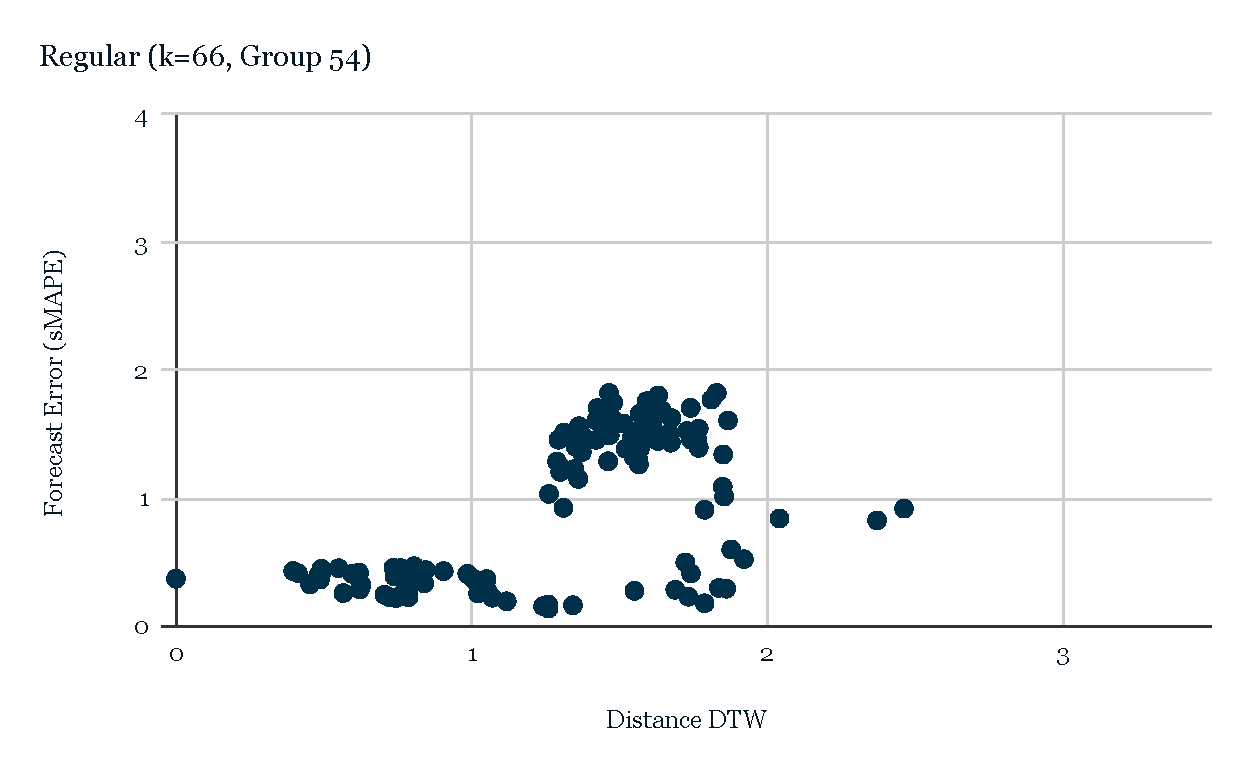
\includegraphics[width=\textwidth]{../Figures/distDTW_ForecastError_r66_c54}
    \caption{Forecast Error with $t_{f}=8$ (for $n=120$ elements) averaged $0.940 \pm 0.551$.}
    \label{Fig:DTWsMAPE_r66_g54}
  \end{minipage}
  \hfill
  \begin{minipage}[b]{0.45\textwidth}
    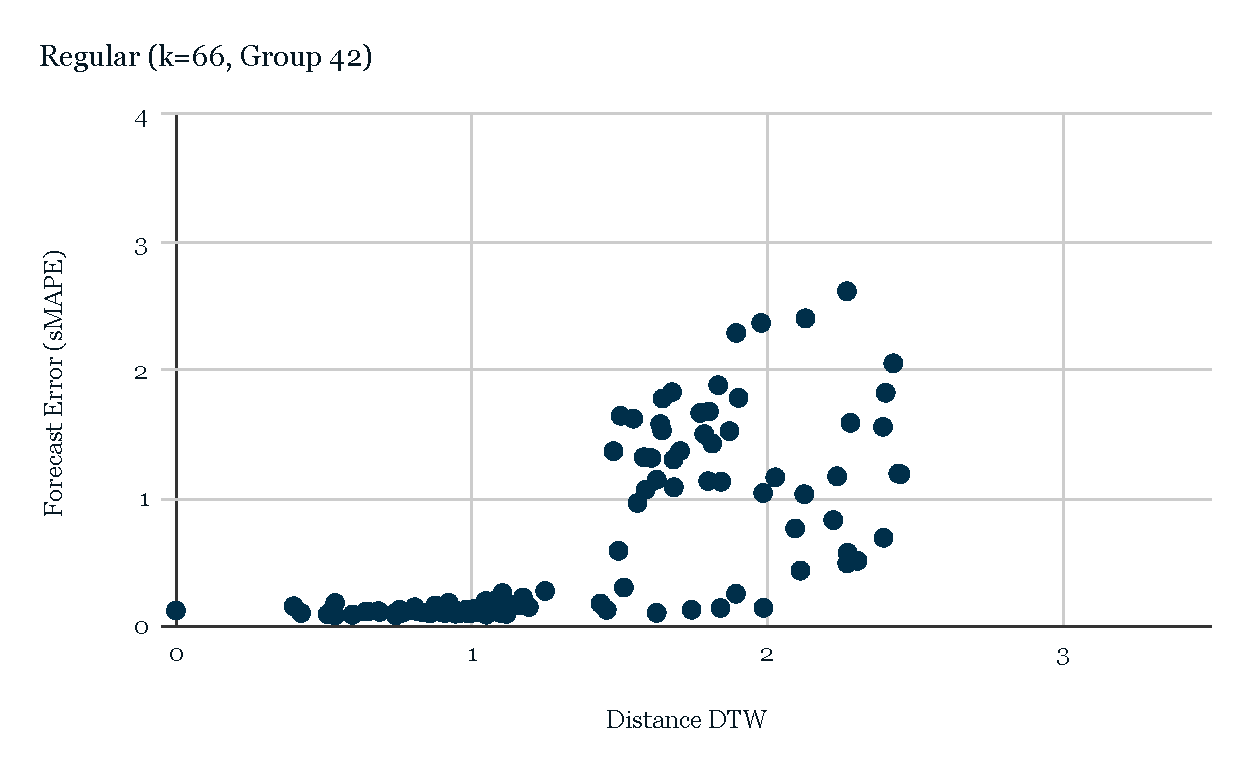
\includegraphics[width=\textwidth]{../Figures/distDTW_ForecastError_r66_c42}
    \caption{Forecast Error with $t_{f}=8$ (for $n=120$ elements) averaged $0.606 \pm 0.684$.}
    \label{Fig:DTWsMAPE_r66_g42}
  \end{minipage}
%\end{figure}

% k=132
%\begin{figure}[!tbp]
  \centering
  \begin{minipage}[b]{0.45\textwidth}
    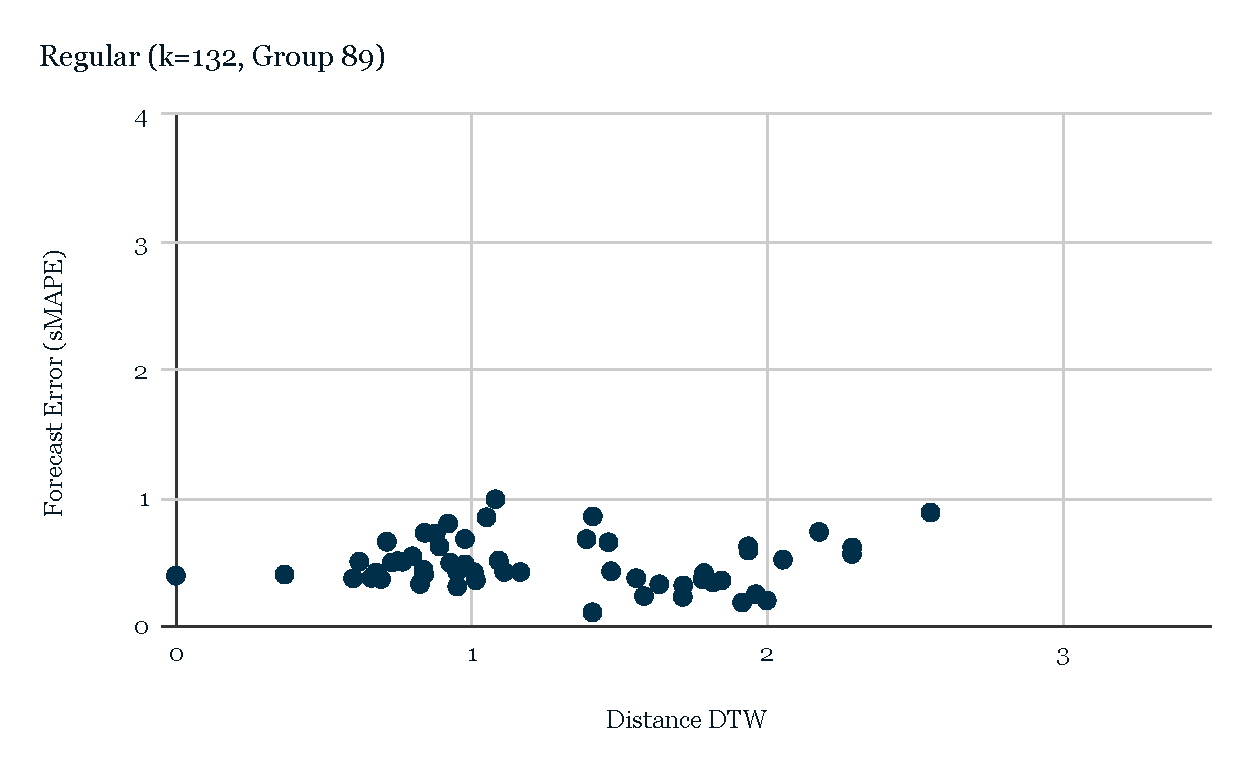
\includegraphics[width=\textwidth]{../Figures/distDTW_ForecastError_r132_c89}
    \caption{Forecast Error with $t_{f}=8$ (for $n=104$ elements) averaged $0.488 \pm 0.188$.}
    \label{Fig:DTWsMAPE_r132_c89}
  \end{minipage}
  \hfill
  \begin{minipage}[b]{0.45\textwidth}
    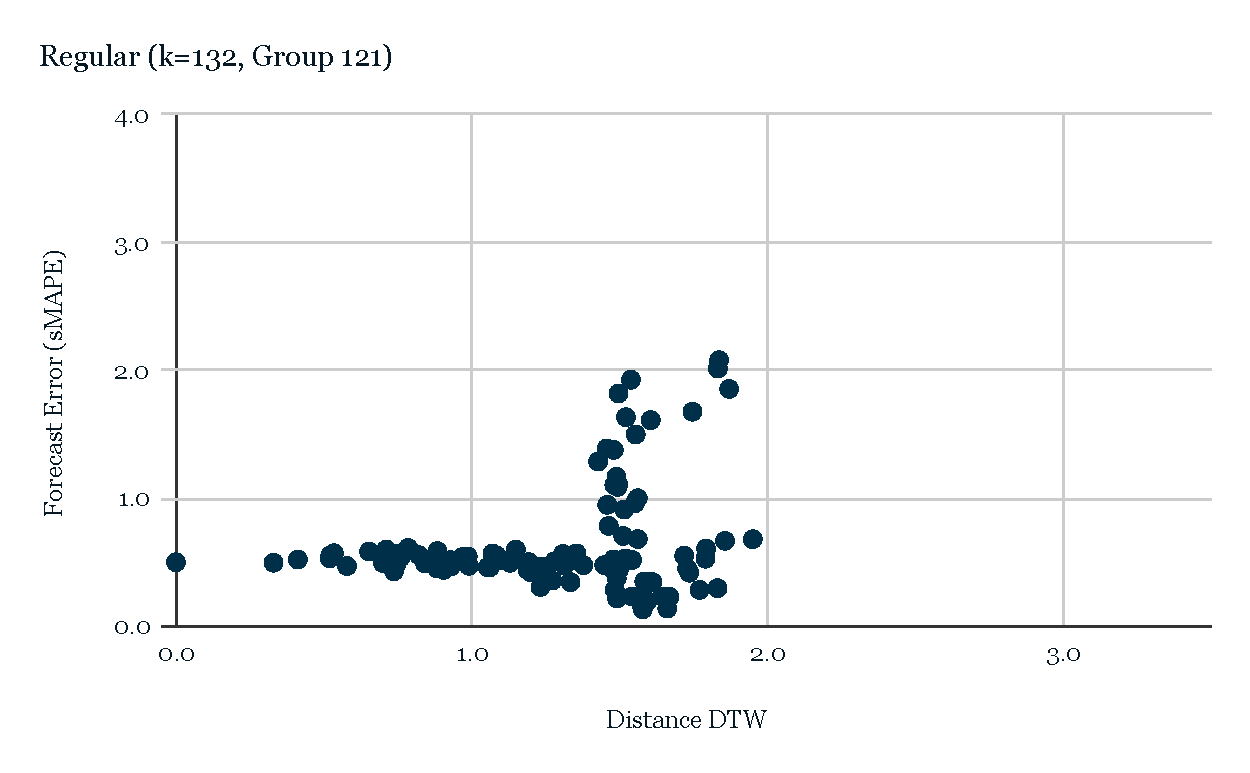
\includegraphics[width=\textwidth]{../Figures/distDTW_ForecastError_r132_c121}
    \caption{Forecast Error with $t_{f}=8$ (for $n=104$ elements) averaged $0.649 \pm 0.431$.}
    \label{Fig:DTWsMAPE_r132_c121}
  \end{minipage}
\end{figure}

\newpage

\section{Predictive Quality of a Model Composition}
\label{Sec:MedoidsModelComposition}

It is now important to remember that there are many different possible model compositions, reviewed in Section \ref{Sec:KnowledgExtraction}. So far, we focused on the `Model Composition of Representative Predictive Models' to show how forecast errors are calculated for a group of elements based on a model calculated at the corresponding representative. 

Model composition is formed by one or more predictors, which will perform a prediction on a domain region. Recalling from Section \ref{Sec:ModelRepresentatives}, the model compositions of interest are the following:

\begin{itemize}%[noitemsep,nolistsep]
	\item Model Composition with Minimal Error (coded `Min.'): for each group in a partitioning scheme, we find the predictive model that minimizes the accumulated forecast error in the group. 
	\item Model Composition with Point Predictive Models (coded `Each'): naive approach where each time series gets its predictive model.
	\item Model Composition of Representative Predictive Models (coded 'Medoid'): for each group, generate a predictive model and apply it to each point in the group.
	\item Model Composition with Maximum Error (coded `Max.'): for each group, we find the predictive model that maximizes the accumulated forecast error in the group.
\end{itemize}

For each of the model compositions above, we use the predictive models trained on a representative model to obtain similar forecast results as those presented in \ref{Sec:AnalyzeForecastErrors} ($t_f =8$ future points, sMAPE error metric). However, here we are interested in a single metric for an entire group of a partitioning scheme. This accumulated forecast error in a group using MSE.

The difference between the different compositions resides only in which representative to use for a given element: once the representative is determined, the procedure in \ref{Sec:AnalyzeForecastErrors} is applied the same (with the same underlying implementation in code). The special cases of `Model Composition with Minimal Error' and `Model Composition with Maximum Error' differ in that the procedure is repeated so that every other element in the group of the given element is considered as a candidate for representative. The representatives with the best and worst aggregated errors are used, respectively.

To summarize the results obtained in the experiments, we compose one table for each partitioning profile technique, $k$-Medoids and Regular (we show the results for $k=8$). The information described in tables \ref{Table:ForecastErrorkMedoidsk8} and \ref{Table:ForecastErrorRegulark10} are the following:

\begin{description}
    \item[Col. 1.] Id cluster group.
    \item[Col. 2.] Number of elements in the group.
    \item[Col. 3.] Parameters $(p, d, q)$ corresponding to the ARIMA model on the representative element (medoid or centroid), obtained with the \texttt{auto.ARIMA} routine.
    \item[Col. 4.] Elapsed time for training all the elements in a cluster group, which corresponds to the naive approach.
    \item[Col. 5.] Elapsed time for performing a prediction for $t_{f}=8$ future points (for all the elements in the domain).
    \item[Col. 6-10.] The MSE aggregation of the sMAPE forecast error for predicting the cluster group, using the model compositions listed above.
\end{description}

\begin{table}[h]
	\centering
	\small
	\begin{tabular}{|c|r|r|r|r|r|r|r|r|r|}
        \hline
        cid & size & $(p, d, q)$ & T. time (s) & F. time(s) & Min. & Each & \cellcolor{red!20}Medoid & Max. \\
        \hline
        0 &  574 & (0, 1, 2) &  2041.469   & 1.069   & 0.161  & 0.170  & \cellcolor{red!20}0.185 & 0.438  \\
        1 &  817 & (2, 1, 2) &  3447.608   & 1.299   & 0.460  & 0.689  & \cellcolor{red!20}0.926 & 1.566  \\
        2 &  542 & (1, 1, 2) &  2011.441   & 0.880   & 0.514  & 0.581  & \cellcolor{red!20}0.678 & 1.420  \\
        3 &  755 & (1, 1, 1) &  2685.912   & 1.238   & 0.289  & 0.413  & \cellcolor{red!20}0.492 & 0.878  \\
        4 & 3479 & (1, 1, 2) & 14542.318   & 5.727   & 0.475  & 0.785  & \cellcolor{red!20}0.838 & 1.983  \\
        5 &  803 & (1, 1, 1) &  3231.718   & 1.375   & 0.294  & 0.407  & \cellcolor{red!20}0.437 & 1.194  \\
        6 &  625 & (3, 1, 1) &  1930.740   & 0.957   & 0.168  & 0.157  & \cellcolor{red!20}0.203 & 0.478  \\
        7 &  505 & (3, 1, 1) &  1811.335   & 0.853   & 0.375  & 0.388  & \cellcolor{red!20}0.551 & 1.015  \\ \hline      
	\end{tabular}
	\caption{Model Composition Forecast Error for Partitioning Domain $k$Medoids with $k=8$ and $t_{f}=8$.}
	\label{Table:ForecastErrorkMedoidsk8}
\end{table}

\begin{table}[h]
	\centering
	\small
	\begin{tabular}{|c|r|r|r|r|r|r|r|r|r|}
		\hline
        cid & size & $(p, d, q)$ & T. time (s) & F. time (s) & Min. & Each & \cellcolor{red!20}Centroid & Max. \\
        \hline
        0 &  990 & (2, 1, 2) &  3601.959 & 1.642 & 0.305 & 0.333 & \cellcolor{red!20}0.331 & 0.826 \\
        1 &  990 & (0, 1, 2) &  3221.489 & 1.665 & 0.180 & 0.192 & \cellcolor{red!20}0.268 & 0.517 \\
        2 &  990 & (1, 1, 2) &  4063.693 & 1.621 & 0.460 & 0.384 & \cellcolor{red!20}0.587 & 1.608 \\
        3 &  990 & (2, 1, 1) &  3424.456 & 1.610 & 0.387 & 0.341 & \cellcolor{red!20}0.394 & 1.028 \\
        4 &  990 & (2, 1, 2) &  4305.636 & 1.651 & 0.571 & 0.782 & \cellcolor{red!20}0.769 & 3.058 \\
        5 &  990 & (1, 1, 2) &  3818.287 & 1.713 & 0.489 & 0.470 & \cellcolor{red!20}0.609 & 2.062 \\
        6 & 1080 & (0, 1, 0) &  4674.208 & 1.744 & 0.564 & 1.190 & \cellcolor{red!20}2.454 & 2.935 \\
        7 & 1080 & (2, 1, 1) &  4847.003 & 1.795 & 0.463 & 0.546 & \cellcolor{red!20}0.583 & 1.188 \\ \hline
	\end{tabular}
	\caption{Model Composition Forecast Error for Regular Partitioning with $k=8$ and $t_{f} =8$.}
	\label{Table:ForecastErrorRegulark10}
\end{table}

% \Fab{vc nao teceu nenhum comentario sobre os resultados em relação ao Erro nas tabelas. Qual a conclusão vc tira desses resultados? Note, não precisa ser um ganho geral..}
% OK
In both tables, we highlight the results of the `Model Composition of Representative Predictive Models'; for all groups in $k=8$ we see that the values are closer to the best possible scenario of `Model Composition with Minimal Error' (obtained by an exhaustive approach) than to the worst scenario `Model Composition with Maximum Error', this already gives some confidence in the results. 

Depending on the number of domain partitions and the number of representatives, we can observe that the aggregated prediction for a region using the model on the representative varies, and experimentally this value exceeds a percentage compared with the naive approach. For $k$-Medoids and $k=8$, the forecast error computed with the model composition of the medoid exceeds in average $20\%$, for $k=66$ in average exceeds $11.3\%$ and for $k=132$ in average exceeds $8.4\%$. These results support our hypothesis that when considering more compact groups, their representative generalizes its elements better. This generalization can be extended to the predictive quality of the representative.

If we add the total time for training the models over all the elements in the naive approach, we get about 31500 seconds. According to these experimental results, to train an ARIMA model using a time series with 349 time instances, the time elapsed on average is $31500 / 8100 \approx 3.9$ seconds. 

In our methodology, we consider train models for $k$ representative elements. Thus the training time for a given partitioning scheme can be estimated as $k \times 3.9$ seconds. So, the total time for training models when maintaining more than one domain partitioning scheme ($k = \{8, 66, 132\}$), is computed by $(8 + 66  + 132) \times 4 \approx 803$ seconds, equivalent to $13.4$ minutes. It is approximately $39$x faster than the naive approach, and this can be contrasted with the relatively low loss of predictive quality.

\subsection{Model Composition for a Domain Region}
\label{Sec:ModelCompositionAggregated}

To further evaluate the forecast error of the `Model Composition of Representative Predictive Models’ approach, we consider the task of predicting the next $t_{f}=8$ for a region of the domain of a fixed size. The objective is to qualify the performance of our solution when faced with spatio-temporal predictive queries. For this, we split the domain using a mesh of size 10x10 (See Figure \ref{Fig:Query_10x10_whole_real_brazil}).

\begin{figure}[ht]
	\centering
	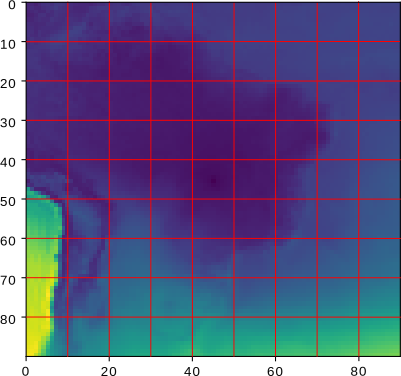
\includegraphics[scale=0.75]{../Figures/query_10x10_whole_real_brazil}
	\caption{Mesh to consider Spatio-Temporal Predictive Queries with Region of size $10 \times 10$.}
	\label{Fig:Query_10x10_whole_real_brazil}
\end{figure}

The results for the resulting $81$ spatio-temporal domain regions are shown in table \ref{Table:Query10x10_kMedoids_Regular_StatSummary}. For each domain partitioning scheme with $k = \left\{8, 66, 132 \right\}$, we present a descriptive statistics summary for the computed forecast error. We can see the variation of mean and standard deviation for the prediction value when considering the model composition formed by the representative models in each domain partitioning technique: $k$-Medoids and Regular.

\begin{table}[h!]
	\centering
	\tiny
	\begin{tabular}{|c|c|c|c|c|c|c|}
		\hline
		\multirow{2}{*}{Dom. Partitioning Technique} & \multicolumn{3}{c|}{$k$-Medoids} & \multicolumn{3}{c|}{Regular} \\
		\cline{2-7}
		& $k = 8$. & $k = 66$ & $k = 132$ & $k = 8$ & $k = 66$ & $k = 132$ \\
		\cline{2-7}
		\hline
		Forecast Error ($t_{f}=8$) & $0.48 \pm 0.59$ & $0.47 \pm 0.86$ & $0.39 \pm 0.62$ & $1.05 \pm 2.07$ & $1.17 \pm 2.59$ & $0.55 \pm 0.68$	 \\
%		Forecast Error ($t_{f}=8$) & $0.48 \pm 0.59$ & $0.47 \pm 0.86$ & $0.39 \pm 0.62$ & $1.05 \pm 2.07$ & $0.45 \pm 0.69$ & $0.44 \pm 0.66$	 \\
		\hline
	\end{tabular}
	\caption{Forecast Error Summary.}
	\label{Table:Query10x10_kMedoids_Regular_StatSummary}
\end{table}

In concordance with the results obtained, the predictions computed by the model composition formed by representative models of the $k$-Medoids technique are consistently more accurate than those obtained with the regular approach. To aid in visualizing these results, we show color maps for the variation of the forecast errors computed in different regions of the domain in Figures \ref{Fig:kMedoid_10x10_k8} to \ref{Fig:Regular_10x10_k132}. Each color map shows the relative intensity of values captured: we assign a dark blue to the highest forecast error, while those lower in their value will be given a lighter blue. The color palette has been kept constant for all figures for visual comparisons.

\begin{figure}[!htbp]
  \centering
  \begin{minipage}[b]{0.45\textwidth}
    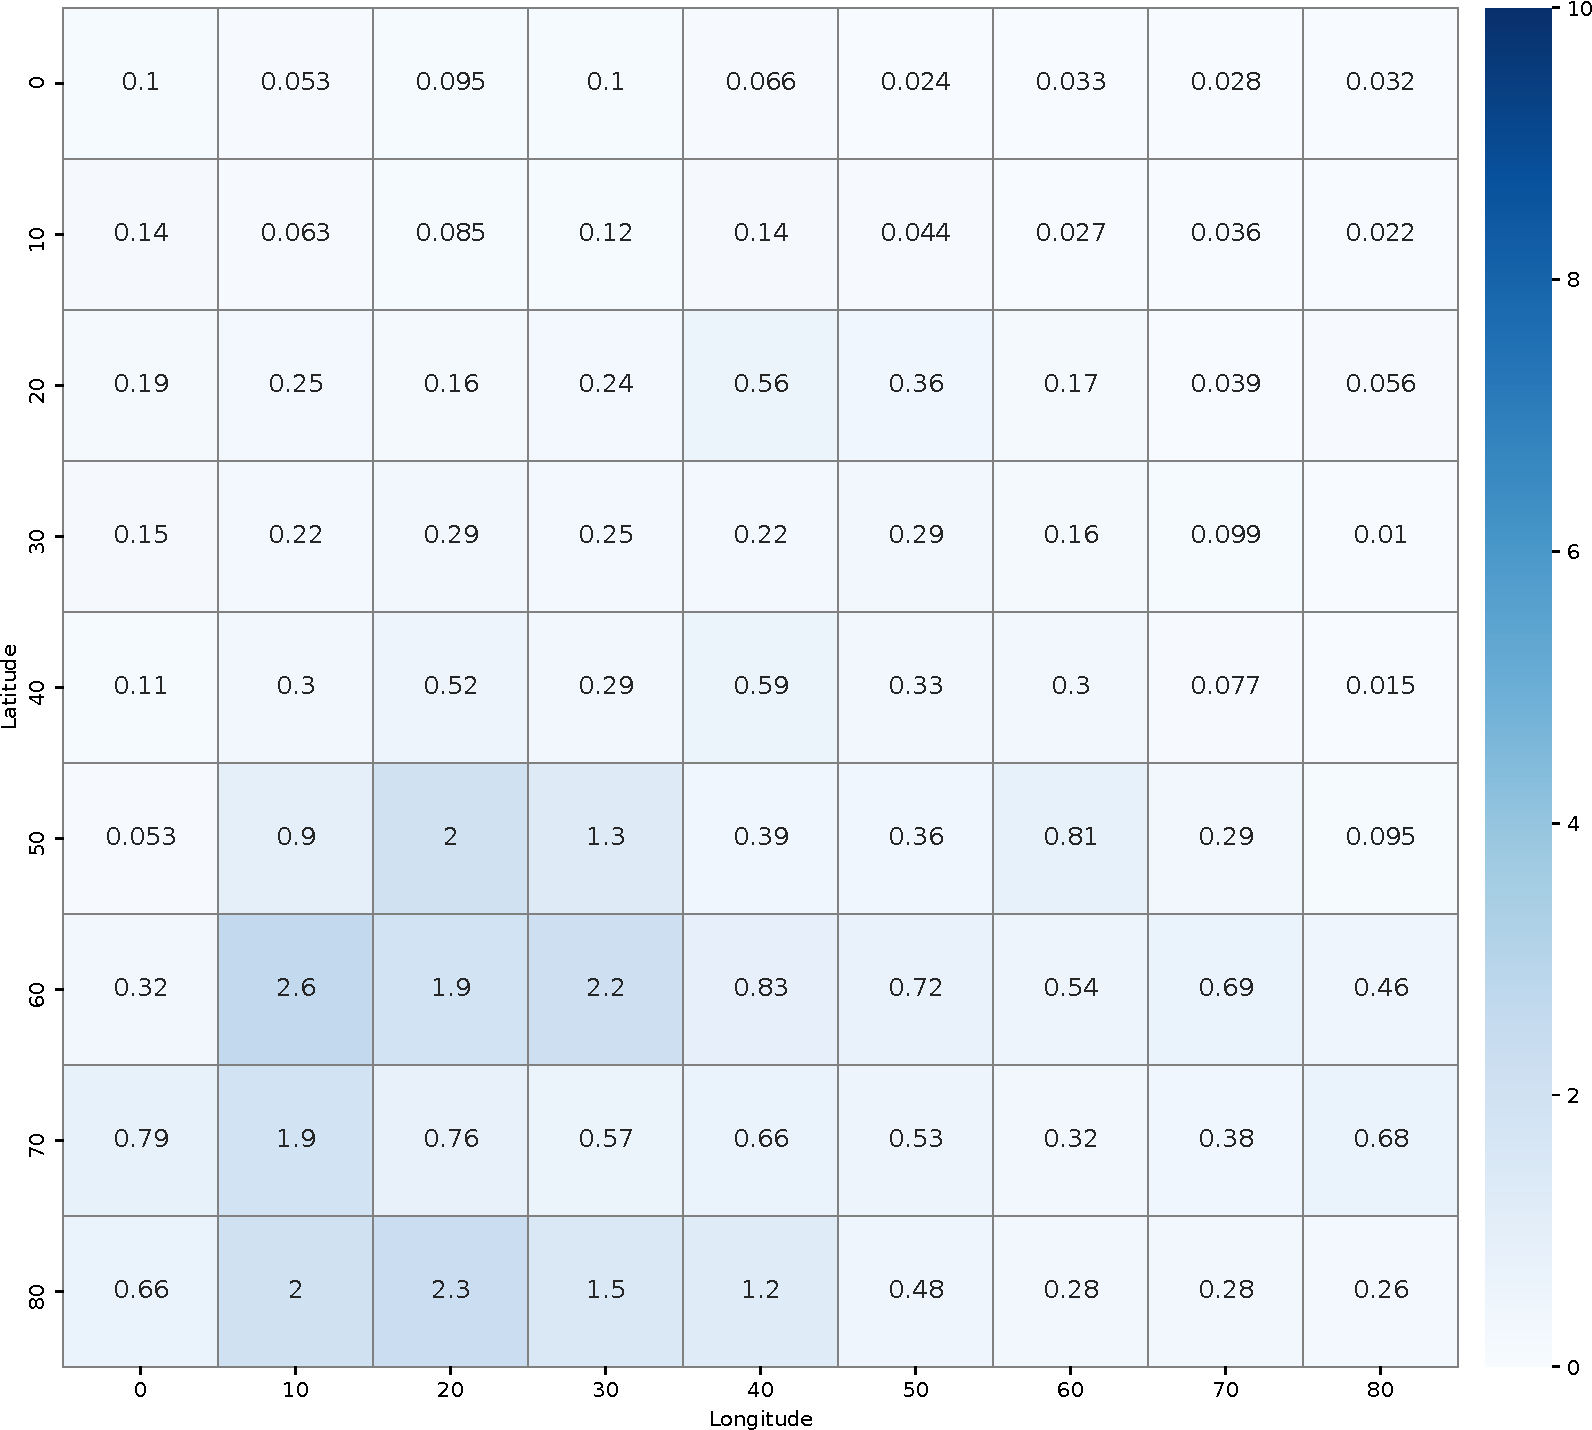
\includegraphics[width=\textwidth]{../Figures/query_10x10_kmedoids_k8-1000dpi}
    \caption{Forecast Error for Model Composition with kMedoids Representatives ($k=8$).}
    \label{Fig:kMedoid_10x10_k8}
  \end{minipage}
  \hfill
  \begin{minipage}[b]{0.45\textwidth}
    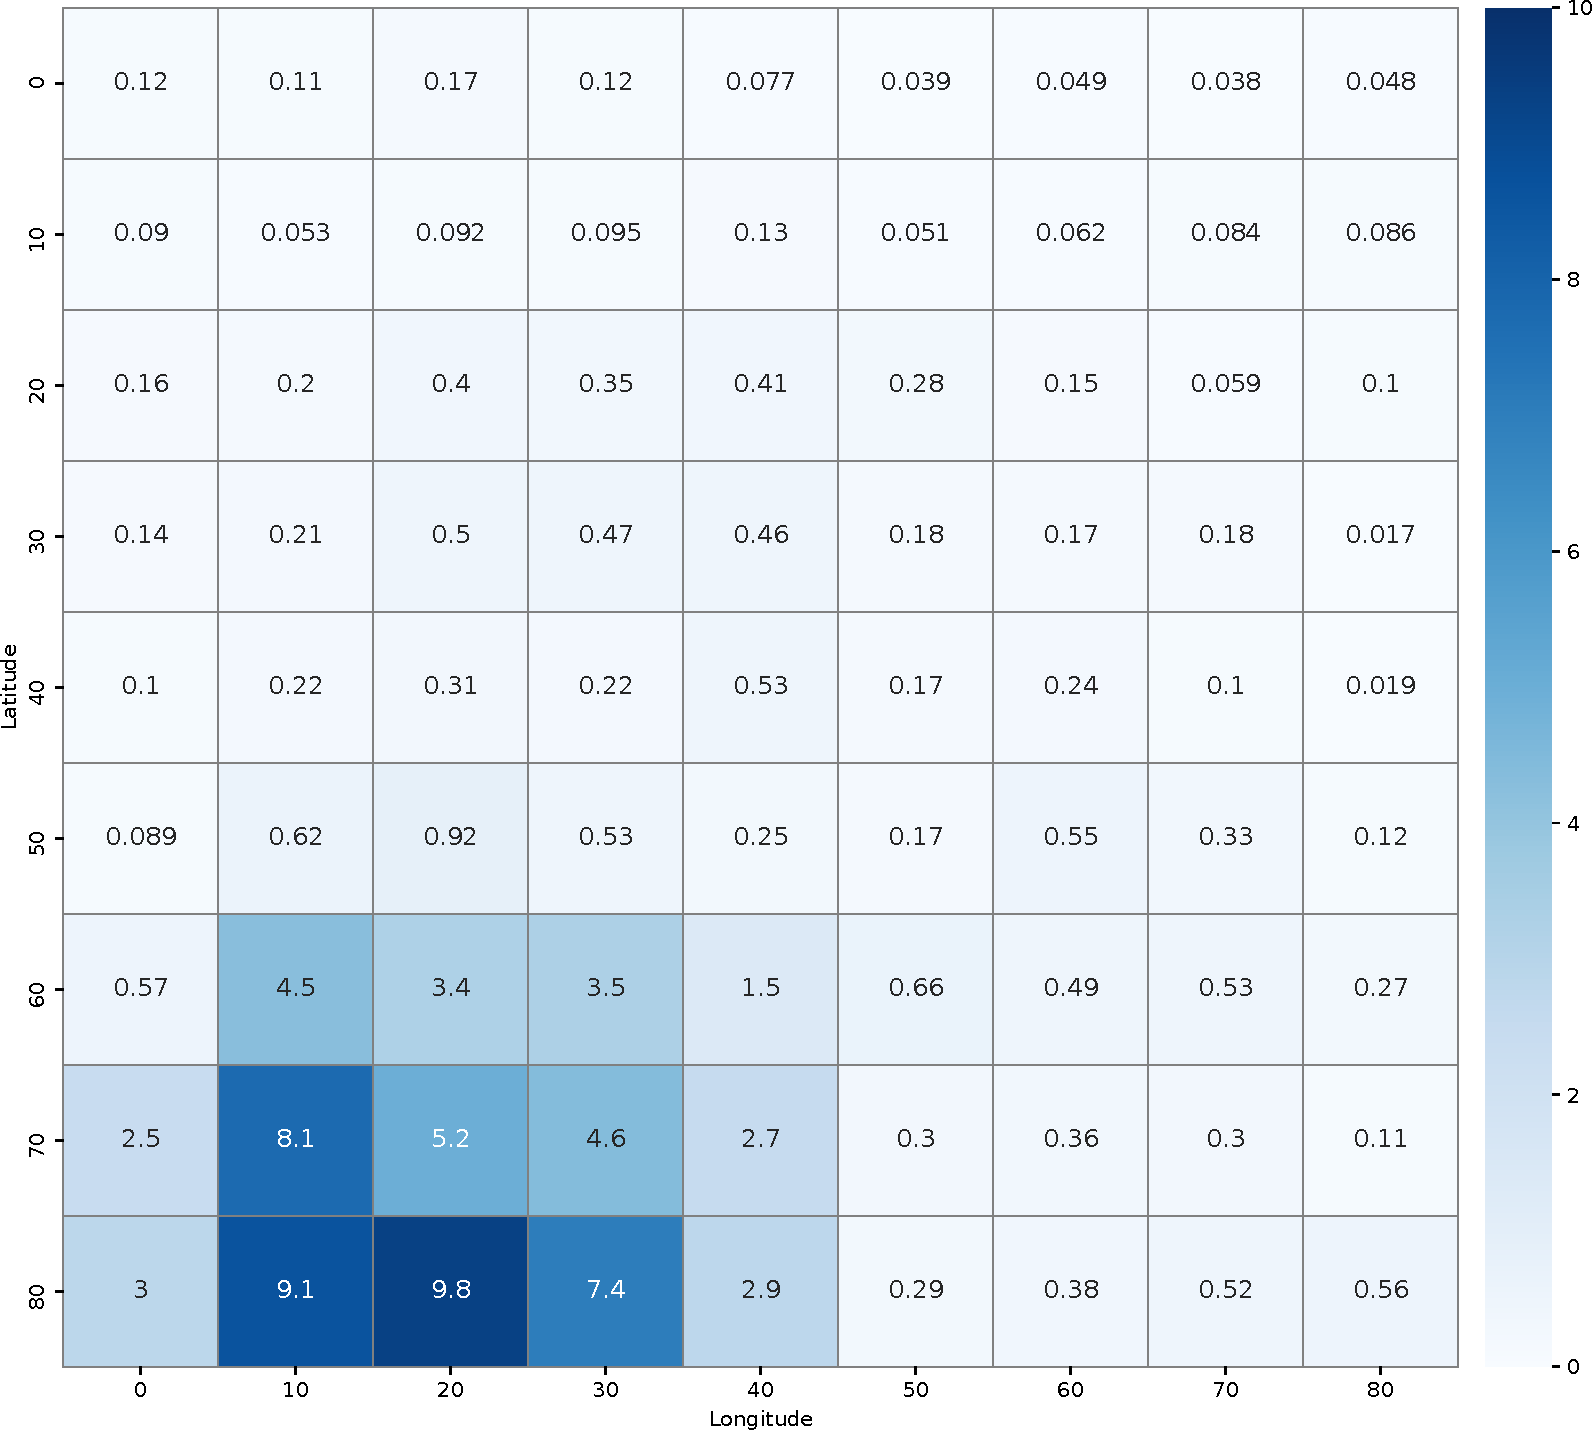
\includegraphics[width=\textwidth]{../Figures/query_10x10_regular_k8-1000dpi}
    \caption{Forecast Error for Model Composition with Regular Representatives ($k=8$).}
    \label{Fig:Regular_10x10_k8}
  \end{minipage}
%\end{figure}

% k=66
%\begin{figure}[!tbp]
  \centering
  \begin{minipage}[b]{0.45\textwidth}
    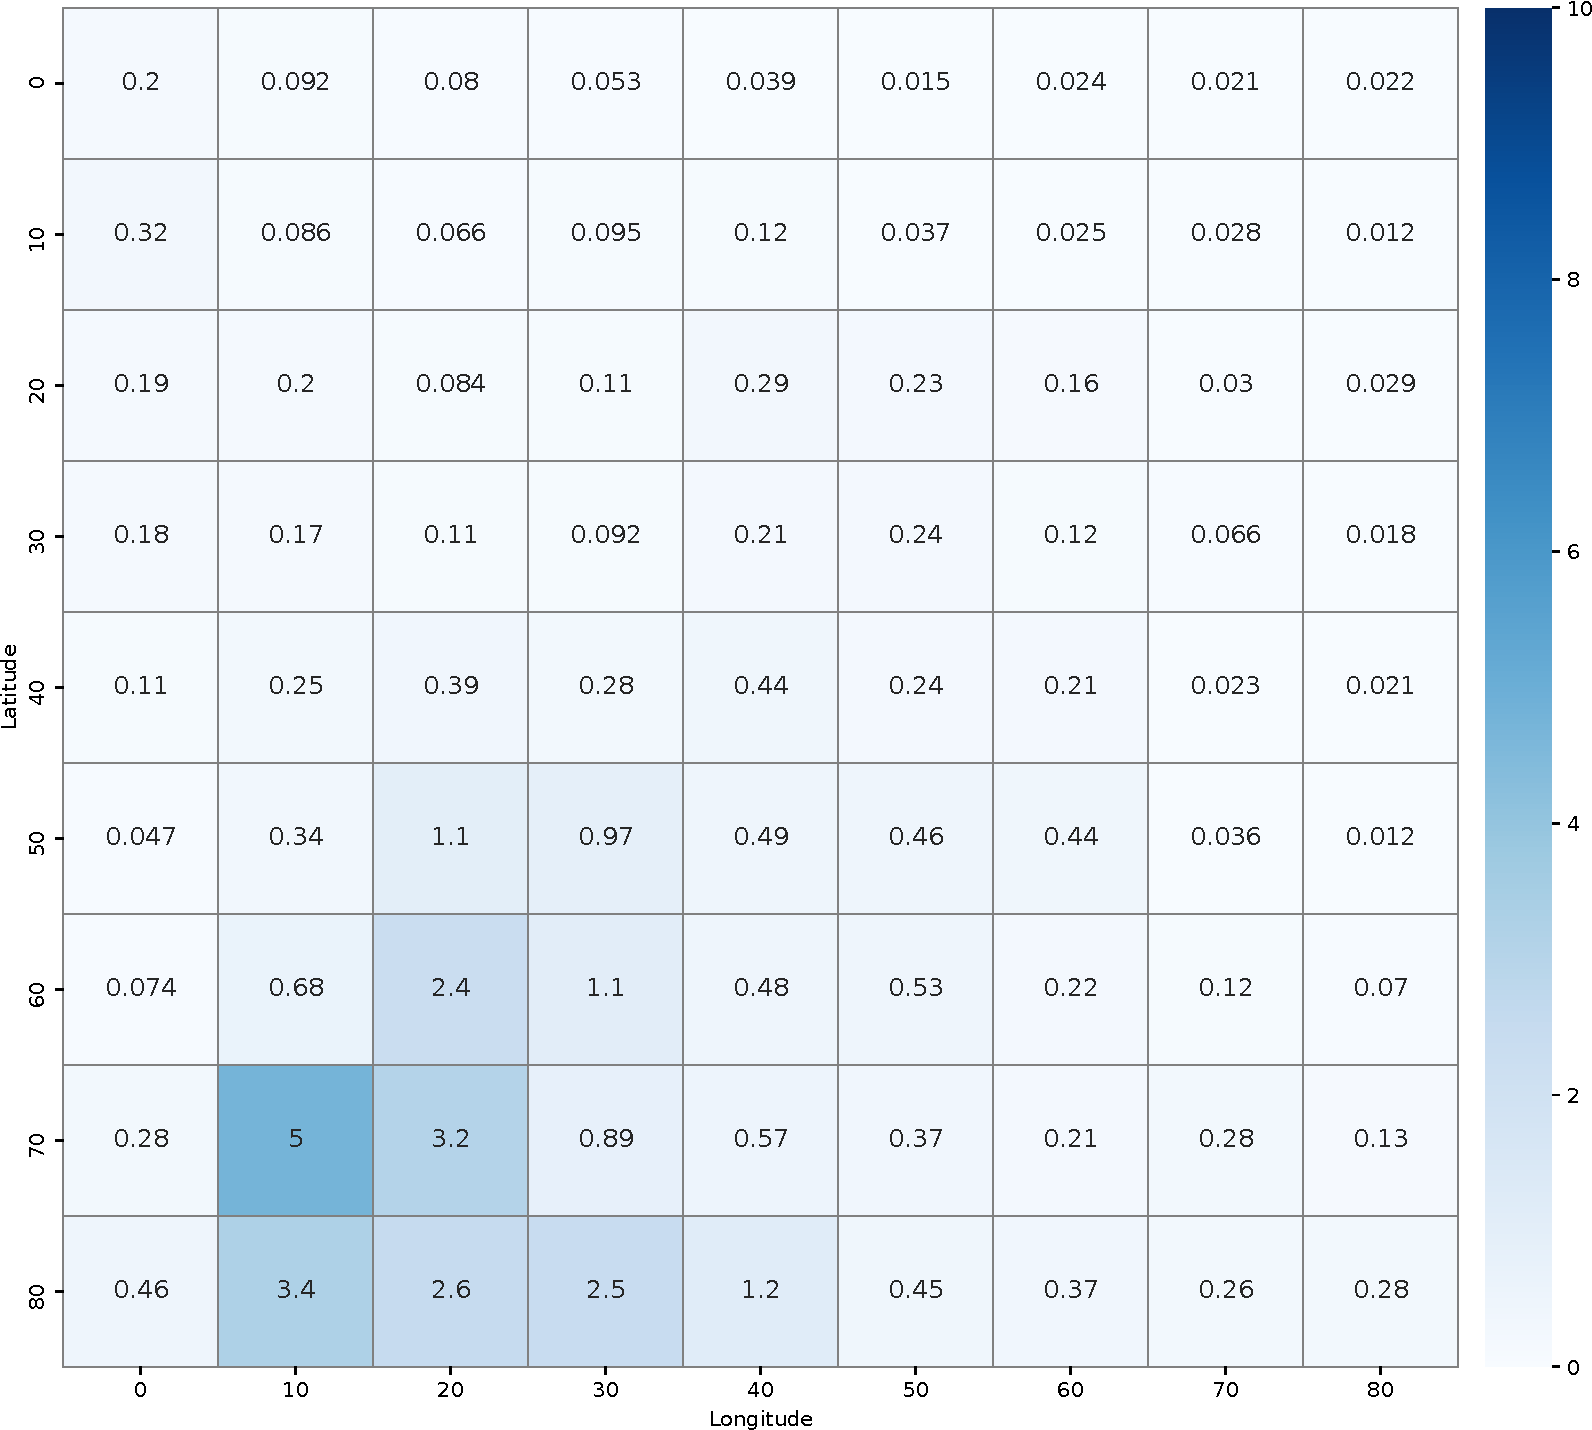
\includegraphics[width=\textwidth]{../Figures/query_10x10_kmedoids_k66-1000dpi}
    \caption{Forecast Error for Model Composition with kMedoids Representatives ($k=66$).}
    \label{Fig:kMedoid_10x10_k66}
  \end{minipage}
  \hfill
  \begin{minipage}[b]{0.45\textwidth}
    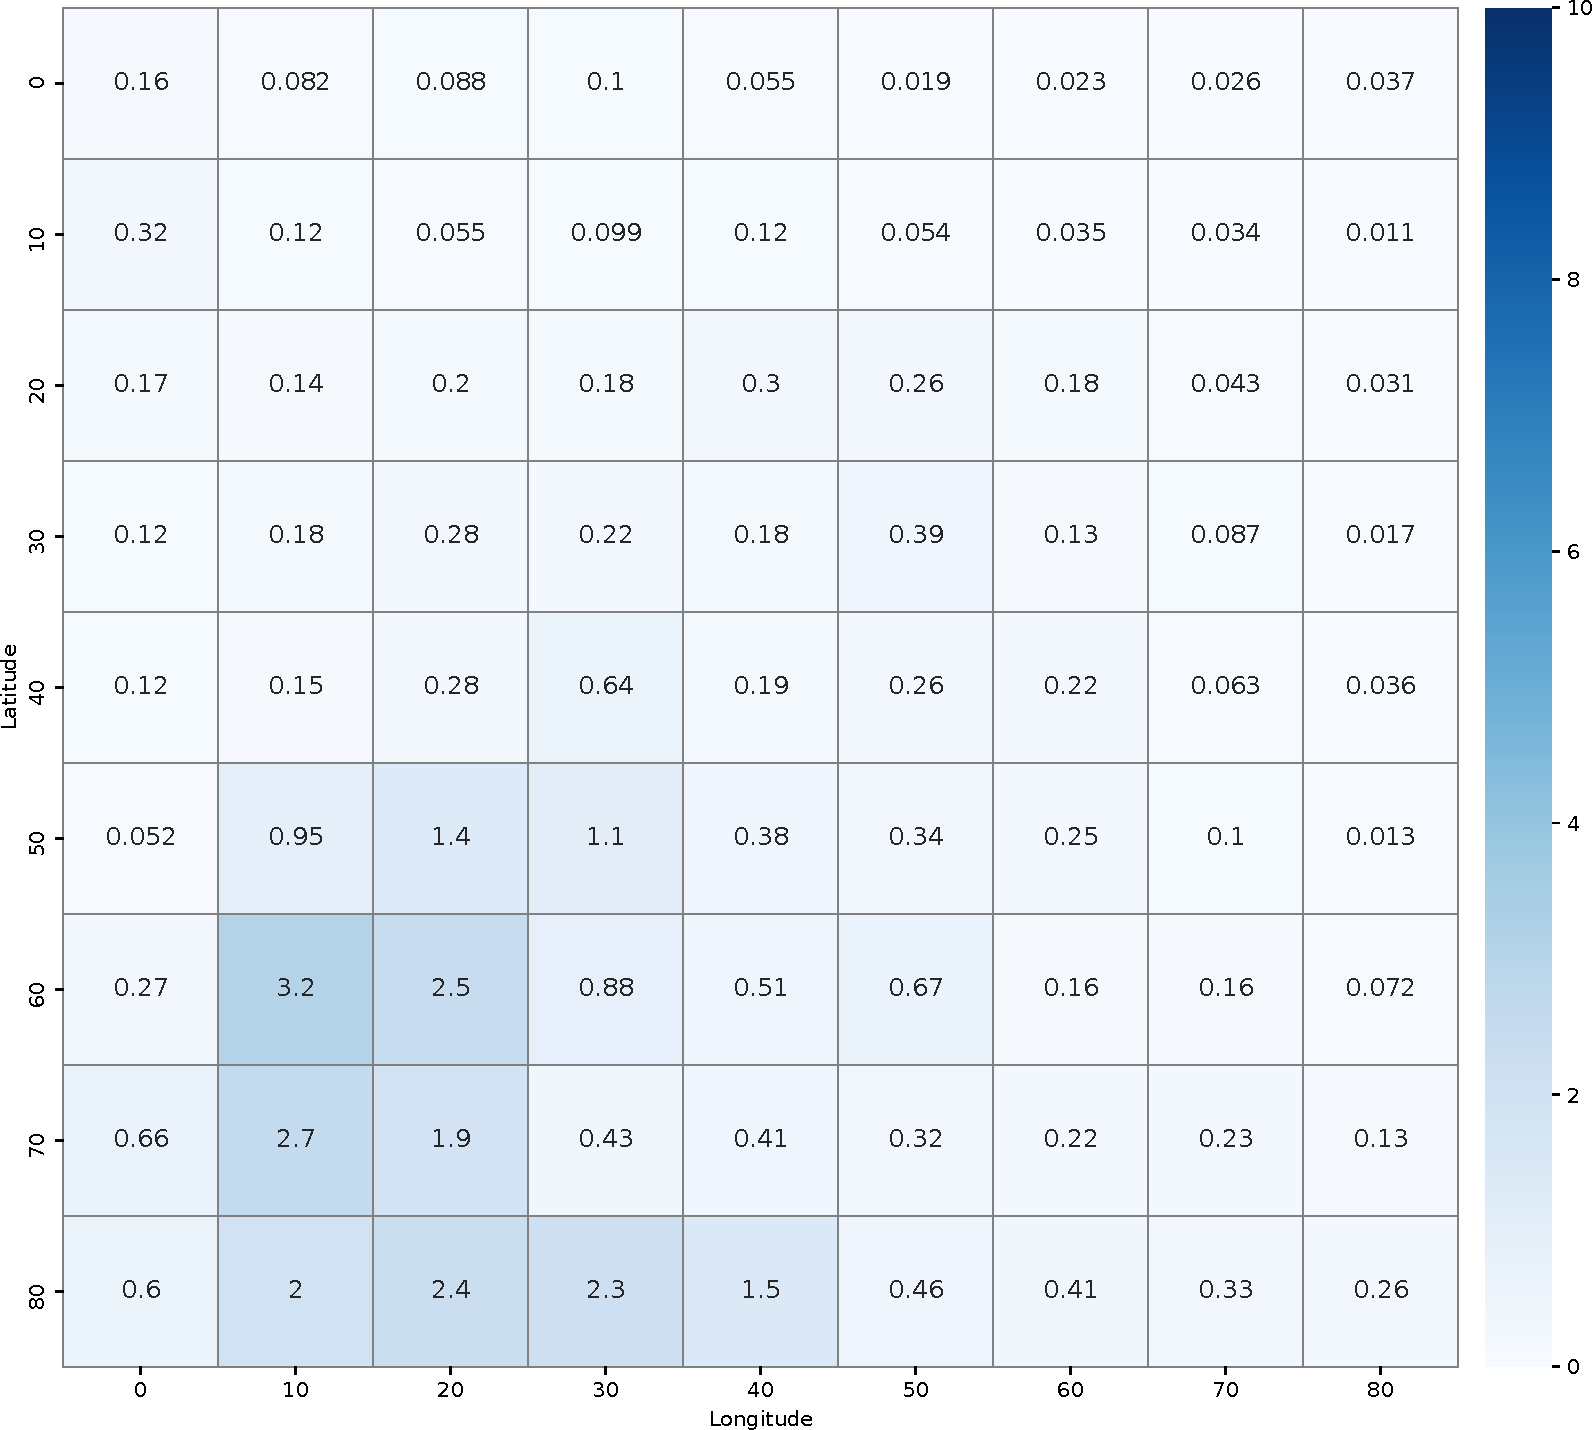
\includegraphics[width=\textwidth]{../Figures/query_10x10_regular_k66-1000dpi}
    \caption{Forecast Error for Model Composition with Regular Representatives ($k=66$).}
    \label{Fig:Regular_10x10_k66}
  \end{minipage}
%\end{figure}

% k=132
%\begin{figure}[!tbp]
  \centering
  \begin{minipage}[b]{0.45\textwidth}
    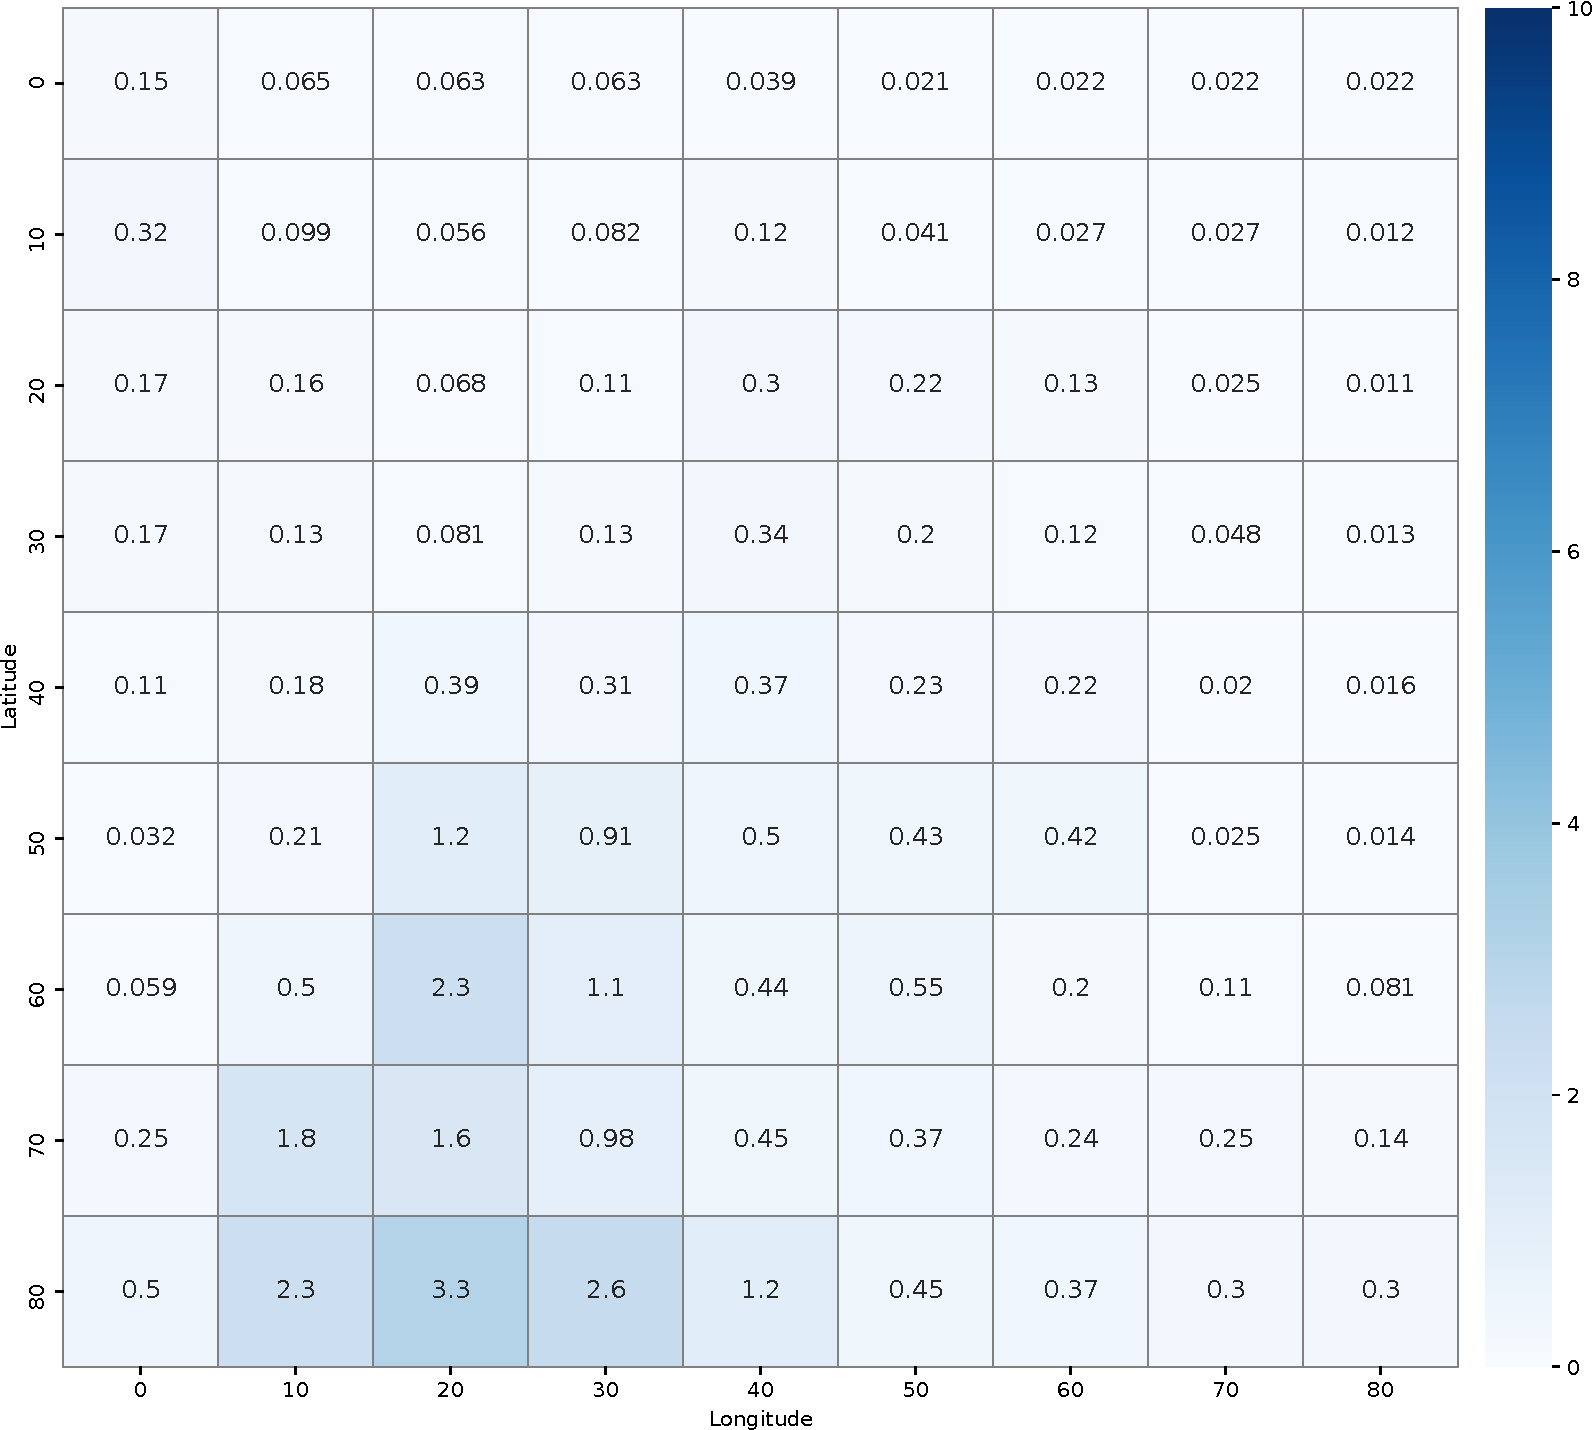
\includegraphics[width=\textwidth]{../Figures/query_10x10_kmedoids_k132-1000dpi}
    \caption{Forecast Error for Model Composition with kMedoids Representatives ($k=132$).}
    \label{Fig:kMedoid_10x10_k132}
  \end{minipage}
  \hfill
  \begin{minipage}[b]{0.45\textwidth}
    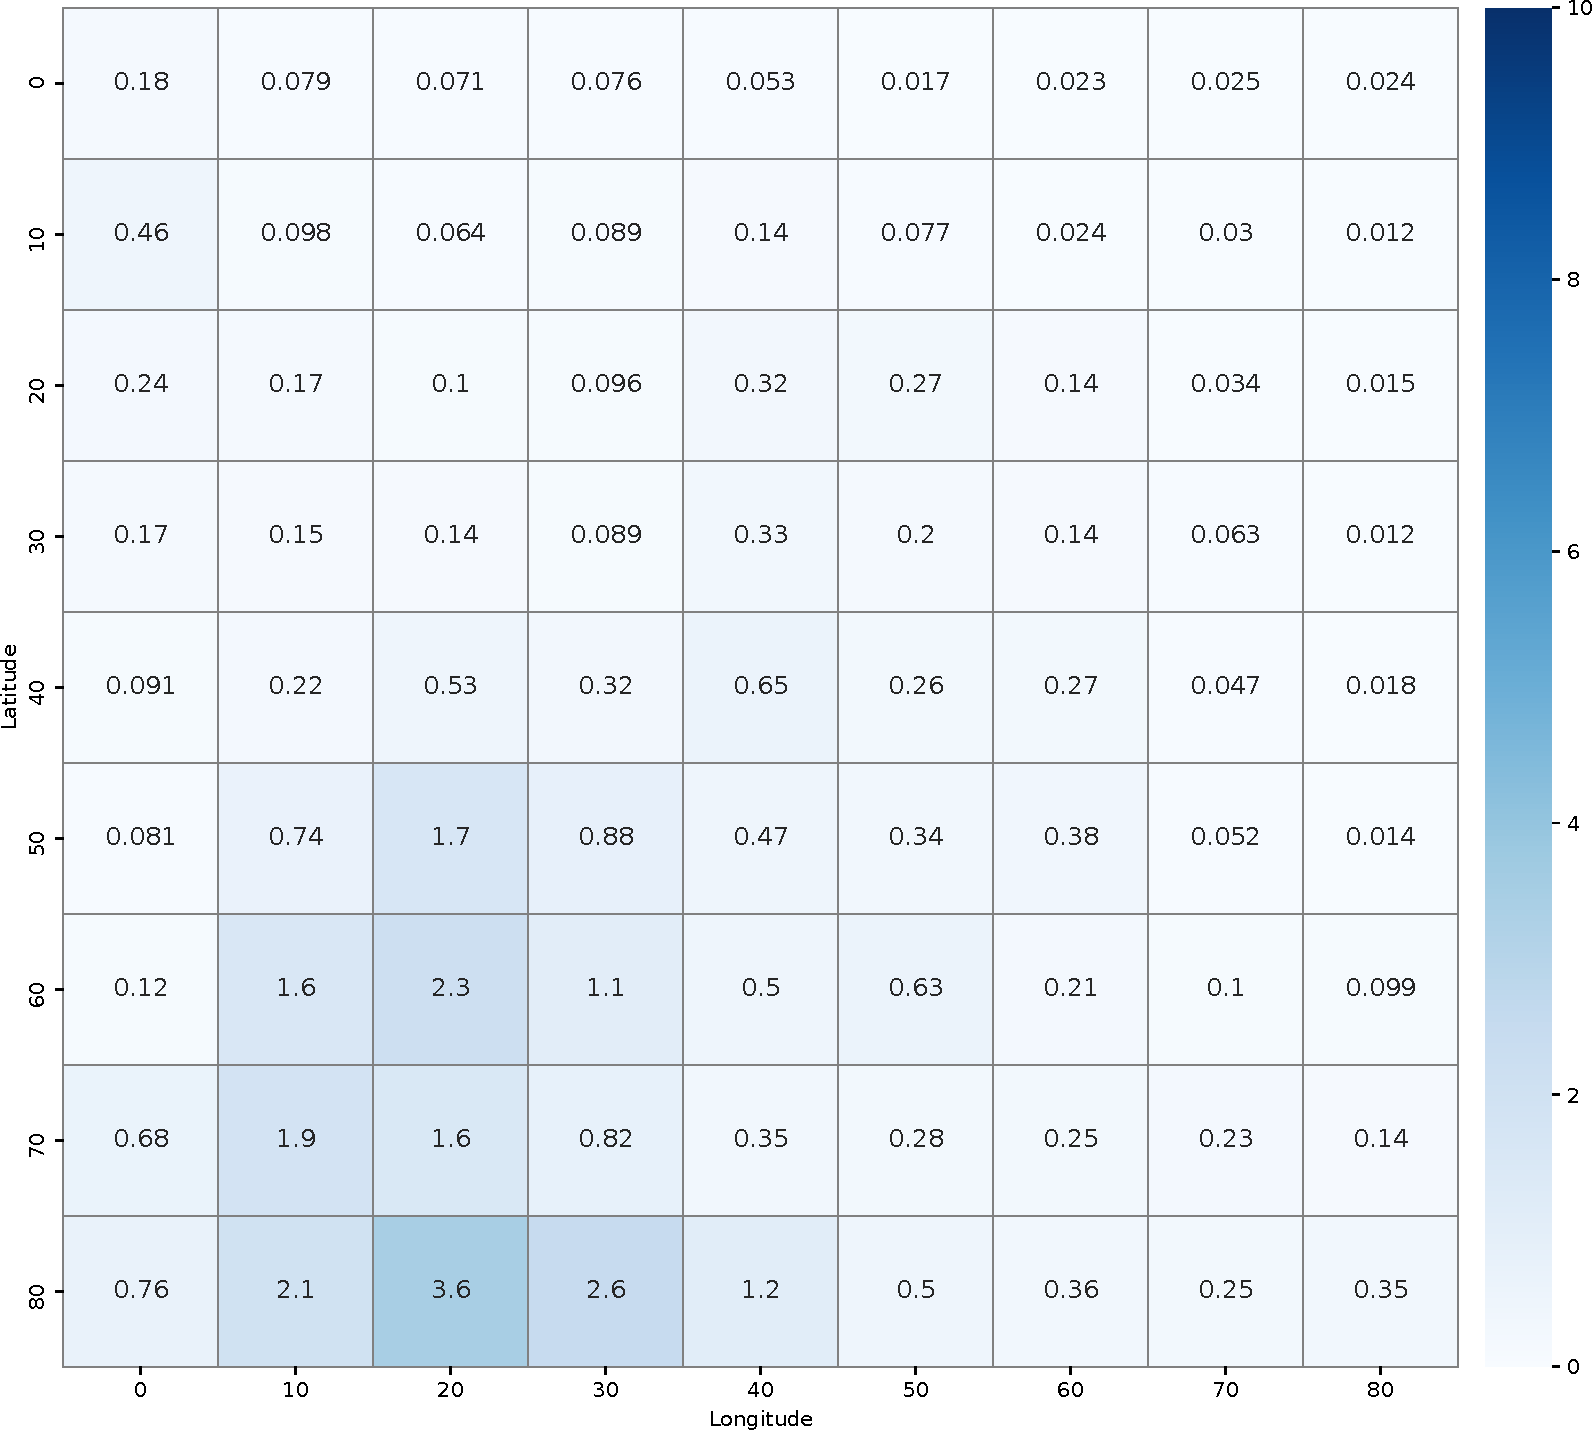
\includegraphics[width=\textwidth]{../Figures/query_10x10_regular_k132-1000dpi}
    \caption{Forecast Error for Model Composition with Regular Representatives ($k=132$).}
    \label{Fig:Regular_10x10_k132}
  \end{minipage}
\end{figure}

Experimentally, we observe that for different values of $k$, the composition of models also presents variations in the prediction values throughout the different slices. It is due to the properties of spatio-temporal data. We further note a particular spatial region near the bottom left, where the forecast error tends to be larger. Also, lower values of $k$ (8, 66) may behave better than $k=132$ for some of the slices. 

The advantage of an off-line process is maintaining various domain division schemes, consequently various predictive models. Their representatives are shown as generalizations of various regions in the domain. The next step is to develop a mechanism that considers the composition of models to predict the temperature in a region of interest, considering the entire set of representatives generated by more than one value of $k$.

\subsection{Preparing a Classifier for Model Selection}
\label{Sec:Classifier}

In this section and the next, we seek to implement a process that can select models using some intelligence to find a composition of models to predict a region of interest with increased accuracy. The justification to implement this step is based on the intrinsic properties of the spatio-temporal data, the consistency and auto-correlation on nearby points in the domain makes difficult the task of finding an 'optimal' number of groups ($k$). Even when we consider the elements only in the temporal dimension, this difficulty persists \cite{Aghabozorgi2015}. In this step, our hypothesis consists in assuming that, if the predictive models on the representatives manage to predict a group of elements (prediction with a certain degree of confidence), based on the similarity of temporal patterns, these models will allow us to reach a prediction for a region of interest of the domain, in which we have only limited information about its past. 

%Introducir la idea del clasificador o porque considero este 
%For now, the desired output  of the classifier is expressed as follows: given a known time series, we want to find a representative among many different partitioning schemes, for which its predictive model can produce an adequate forecast.
For now, the desired output of this step could be expressed as follows: given a known time series, we want to find a representative among many different partitioning schemes, for which its predictive model can produce an adequate forecast.

Here, it is necessary to remember that, when computing the future value of a variable for a time series, we have to consider a range of values in the immediate past\cite{Chatfield2001}. Thus, to create a process for selecting models, we need a mechanism that allows us to find and use relationships between the set of representatives and past temporal instances of every element in the region of interest (See Figure \ref{Fig:model_composition_classifier_diagram}).

\begin{figure}[h]
	\centering
	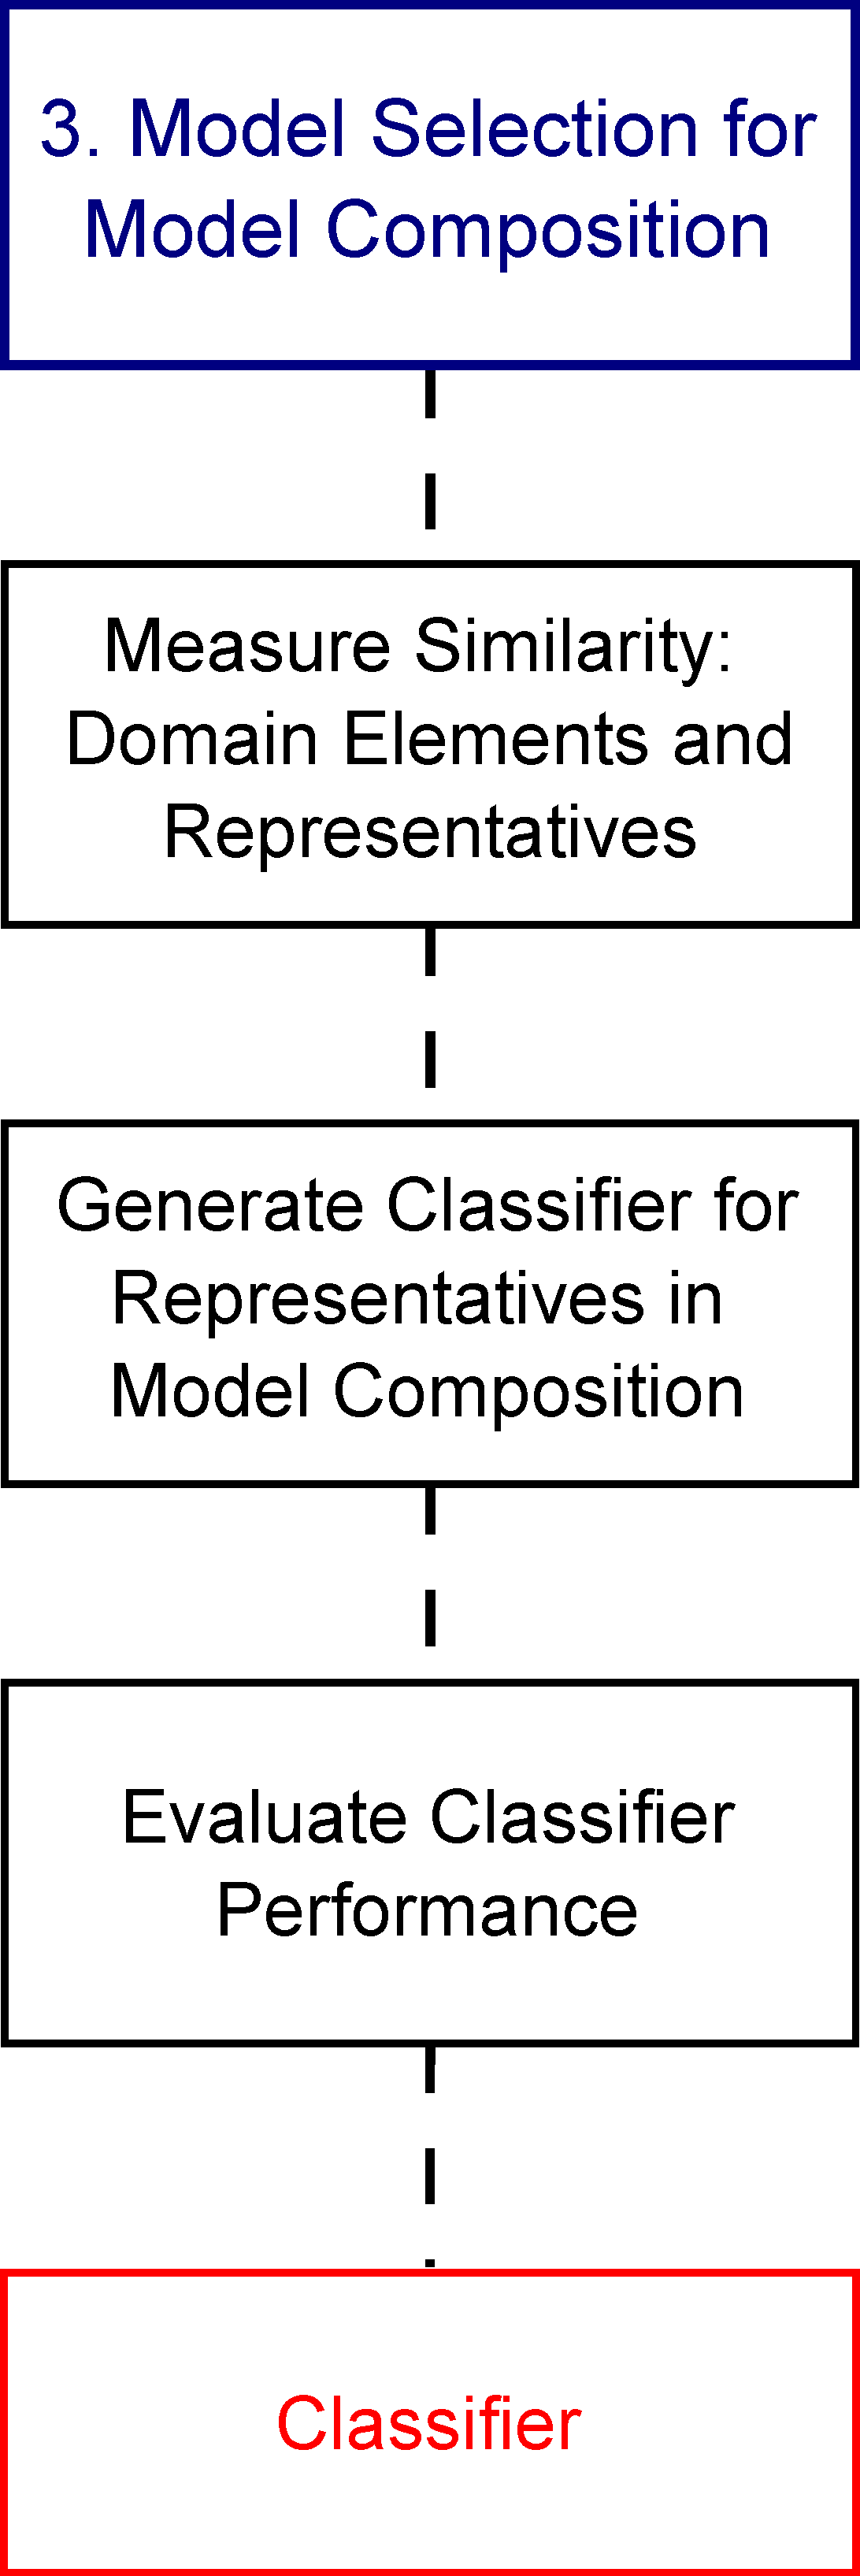
\includegraphics[scale=0.15]{../Figures/Experiments_Methodology_Step3}
	\caption{Model Composition using the Classifier Approach.}
	\label{Fig:model_composition_classifier_diagram}
\end{figure}

We formulate this step as a univariate time series multi-class classification problem: Given an unlabeled univariate time series, assign it to one or more predefined classes. We consider the classes to be the identifiers of models computed at the representatives for each cluster. The time series takes part whenever multiple clustering is applied to the domain dataset. Thus, if a time series participates of two clusters, with $k_1$ and $k_2$ respectively, it would have associated two models $g_1$ and $g_2$ as labels. The label is composed with the value $k$ and the group index \texttt{cluster\_index} (c.i) where $0 \leq c.i <k$.

In order to show how we can leverage domain partitioning schemes and their respective representatives, we use the formal representation of the problem (see Section \ref{Sec:ProblemFormalization}). With three different domain partitioning schemes as an example: Given three domain partitioning schemes for a spatio-temporal domain of sizes $m, n$ and $l$ and their respective representative sets, we have:
\begin{eqnarray} 
\nonumber
\mathcal{D}	& = & \bigcup_{i=1}^{m} \mathbf{P_i} \,\,\textrm{and} \,\, \left\{\mathcal{P}_{1}, \ldots, \mathcal{P}_{m}\right\}, \\ \nonumber
\mathcal{D} & = & \bigcup_{j=1}^{n} \mathbf{Q_j} \,\,\textrm{and} \,\, \left\{\mathcal{Q}_{1}, \ldots, \mathcal{Q}_{n}\right\}, \\ \nonumber 
\mathcal{D} & = & \bigcup_{k=1}^{l} \mathbf{T_k} \,\,\textrm{and} \,\, \left\{\mathcal{T}_{1}, \ldots, \mathcal{T}_{l}\right\},
\end{eqnarray}

where $m, n, l < \textrm{card}(\mathcal{D})$. The set of representatives on the partitioning schemes considered is $\mathbf{R} = \left\{\mathcal{P}_{i}, \ldots, \mathcal{P}_{m}, \mathcal{Q}_{1}, \ldots, \mathcal{Q}_{n}, \mathcal{T}_{1}, \ldots \mathcal{T}_{l} \right\}$ , and $\mathcal{G}_{(\mathbf{R})}$ is the set of their correspondent models. Now, for an arbitrary element $\mathcal{S}$ in the domain, we want to find a representative $\mathcal{\hat{S}} \in \mathbf{R}$ of some group in a partitioning scheme, so that satisfies some optimization condition. Here we consider the representative $\mathcal{\hat{S}}$ such that has the minimum DTW distance with $\mathcal{S}$:

\begin{equation}\label{eq:timeseries-representative}
 \exists\, \mathcal{\hat{S}} \in \mathbf{R}, \,\, \textrm{such that}, \,\, \argminA_{\substack{\mathcal{\hat{S}} \in \mathbf{R}\\\mathcal{S} \in \mathcal{D}}} d_{DTW}(\mathcal{\hat{S}}, \mathcal{S}).
\end{equation}

In order to simplify the notation of the aforementioned relationship (\ref{eq:timeseries-representative}), we denote the representative with a label \texttt{[number\_of\_clusters, cluster\_index]}. Assuming that only the number of clusters is used as a parameter for partitioning schemes, this label can uniquely identify each of the representative models to extract a 'Time Series Classification Dataset ($TSCD$)`, similar to Table \ref{Tab:TSClassificationDataset}.

\begin{table}[h]
	\centering
	%	\tiny
	\begin{tabular}{|c|c|}
		\hline
		Time-Series & Label for the Representative Model\\ \hline
		$\mathcal{S}_{1}$ & \texttt{[m, 1]} \\ \hline
		$\mathcal{S}_{2}$ & \texttt{[l, l-1]} \\ \hline
		$\mathcal{S}_{3}$ & \texttt{[n, n-2]} \\ \hline
		$\mathcal{S}_{4}$ & \texttt{[l, 2]} \\ \hline
		$\mathcal{S}_{5}$ & \texttt{[m, m-1]} \\ \hline
		$\vdots$ & $\vdots$ \\ \hline
	\end{tabular}
	\caption{Dataset of time series and labels satisfying relationship (\ref{eq:timeseries-representative}) for domain partitioning sizes $(m,n,l)$.}
	\label{Tab:TSClassificationDataset}
\end{table}

\subsection{Training a Classifier for Model Selection}
\label{Sec:TrainingClassifier}

% Idea of Classifier
For the second part of the model selection process, we are interested in implementing a mechanism based on the knowledge acquired on an extracted dataset $TSCD$ (Table \ref{Tab:TSClassificationDataset}). The objective is, given a previously unseen time series, to infer a suitable label (and thus a predictive model on a representative) for it by recognizing patterns in the time series. It can be formulated as a time-series classification problem, which consists of training a classifier on a dataset $TSCD$ in order to map from the space of possible inputs to a probability distribution over the class variable values (labels).  

With the proposed classification method, we will be able to learn from data about the membership relation between elements of the domain and representatives, and then use this learned knowledge to classify new time series. A dataset $TSCD=\{(\mathcal{S}_1,y_1),(\mathcal{S}_2,y_2), \ldots ,(\mathcal{S}_N,y_N)\}$ is a collection of pairs $(\mathcal{S}_i,y_i)$ where $\mathcal{S}_i$ is univariate time series with $y_i$ as its corresponding one-hot label vector of the labels \cite{Gulli2017}. For a dataset containing $m+n+l$ classes, the one-hot label vector $y_i$ is a vector of length $m+n+l$ where each element $j \in [1,(m+n+l)]$ is equal to 1 if the class of $X_i$ is $j$ and $0$ otherwise \cite{Mitsa2010}.

% Multiclass classifier
The task of time series classification is not a simple one. Considering the sequential aspect of time series data requires the development of algorithms that can harness this temporal property to select a class label from among a collection of candidates. While many neural network architectures can solve this problem, some work better than others \cite{Bagnall2017a}.

In this work, we use Convolutional Neural Networks (CNNs). They typically fare very well on multiclass classification tasks, especially for images and text \cite{Goodfellow2016}. The powerful learning ability of deep CNN is primarily due to multiple feature extraction stages that can automatically learn representations from the data. Research has shown that using CNNs for time series classification has several advantages over other methods; they are highly noise-resistant models. They can extract very informative, deep features independent of time \cite{Wang2016, Bagnall2017a, Zhao2017}.

% https://monkcage.github.io/blog/ai/2019/01/28/time_series_forecast.html
% CNN-LSTM for Time Series Classification
Another architecture is the Long-Short Term Memory Neural Networks (LSTM). The benefit of this model is that it can support very long input sequences. By implementing a hybrid CNN-LSTM Neural Network, we can integrate the capacity of process time series as blocks or sub-sequences by the CNN model, then pieced together by the LSTM model. Then the model will further divide each sample into further sub-sequences. The CNN model will interpret each sub-sequence, and the LSTM will piece together the interpretations from the sub-sequences. 

% TODO we got what we wanted, a system that can receive a time series as input, and return a representative model as output.
\section{Building a Classifier}
\label{Sec:ExperimentsTrainingClassifier}

In Sections \ref{Sec:Classifier} and \ref{Sec:TrainingClassifier} of our proposed methodology, we describe the implementation of a Neural Network Model for the Time Series Multiclass Classification task. Here, we show how we build a classifier using the extracted dataset and known domain partitioning schemes as input. We want to leverage the three partitioning schemes for $k = \{8, 66, 132\}$, obtained in Section \ref{Sec:Selectk} through selection and their corresponding predictive models on representatives. The goal is to obtain a new model composition similar to the `Model Composition of Representative Predictive Models' (see Section \ref{Sec:KnowledgExtraction}), but where the representatives are dictated by the classifier instead of just the group that a given sample belongs. 

\subsection{Generating Dataset}
\label{Sec:ClassifierDataset}

In the previous sections, the experiments performed to evaluate the predictive quality (forecast) of the models on representatives, which were determined by the $k$-medoids algorithm. As a result, we can see that when more than one partitioning scheme of the domain is considered, different models for a region have the potential for better predictive quality.

%According to the proposed methodology, we want to implement an algorithm that allows classifying the domain elements in a set of classes. These classes are determined by the representative and the elements are those that present the minimum similarity (DTW distance) between them (See Section \ref{Sec:Classifier}.  

In Section \ref{Sec:Classifier}, we discussed how the classifier would be used to categorize the domain elements into a set of classes. Each of these classes corresponds to a representative of one of the available partitioning schemes. Considering the partition schemes of sizes $k=\{8, 66, 132\}$, we obtain $183$ classes in total, after accounting for repetition of medoids between the schemes.

In order to work with a balanced dataset, we extract for the $TSCD$ approximately $30$ samples per class \cite{Du2018}. In total, we consider 5000 samples. We divide the dataset in the percentages $60/20/20$ for training, validation, and test, respectively.

Then, we process the $TSCD$ dataset so that each example is formed by a time series $\mathcal{S}$ and a label $y$. The label is a tuple representing both the domain partitioning scheme and one of the $k$ groups in the resulting partition (and by extension, uniquely identifies a predictive model in a representative) of a partitioning technique.

\begin{table}[h]
	\centering
	\small
	\begin{tabular}[h]{|c|c|c|c|c|c|c|c|c|c|}
		\hline
		  & s0    & s1    & s2    & s3    & s4    &	s5    & $\ldots$ & s364  &   label \\ \hline
		0 & 0.484 & 0.563 & 0.443 & 0.386 & 0.326 &	0.391 & $\ldots$ & 0.359 &   8-3 \\
		1 &	0.482 &	0.508 &	0.520 &	0.477 &	0.354 &	0.444 & $\ldots$ & 0.361 & 132-69 \\
		2 &	0.639 & 0.618 &	0.549 &	0.609 &	0.433 & 0.476 & $\ldots$ & 0.421 &	66-26 \\ 
		$\vdots$  & &     &       &       &       &       &          &       & $\vdots$ \\ \hline
	\end{tabular}
	\caption{Dataset extracted for the Time Series Classification Task.}
	\label{Table:DatasetTSC}
\end{table}

The neural network models learn a mapping from input variables to an output variable. A model with large weight values is often unstable, meaning that it may suffer from poor performance during learning and sensitivity to input values resulting in higher generalization error \cite{Lecun1998}. Differences in the scales across input variables may increase the difficulty of the problem being modeled. To avoid this we normalize the dataset (Table \ref{Tab:TSClassificationDataset}). Next, we describe the architectures considered and their properties.

\subsection{Classifier Architectures and Results}
\label{Sec:TSC_NN_Results}

% Architectures considered
We consider the following architectures: Long-Short-Term Memory (LSTM), Convolutional Neural Network (CNN), and a hybrid CNN1D-LSTM (see Sections \ref{Sec:DL-TSC} and \ref{Sec:TrainingClassifier} for details). The architecture hyperparameters for these two architectures and the hybrid version are listed in Table \ref{Table:HyperparametersNN}; the corresponding optimization parameters are shown in Table \ref{Table:OptimizationNN}. In the first table, we list the number and type of layers and their respective activation function, Rectified Linear Unit (ReLU). We consider a downsample option for the CNN architecture to accelerate the computation using the pooling layer for 1D temporal data \cite{Gholamalinezhad2020}. To avoid overfitting, we opt for the regularization technique dropout \cite{Srivastava2014, Baldi2013}. 

The architectures considered in this work are based on models for univariate time series classification\footnote{http://www.timeseriesclassification.com}, proposed in works such as \cite{Bagnall2017a, Fawaz2019}. Due to the domain size, we consider models with a reduced number of layers.

All models were optimized using a variant of Stochastic Gradient Descent such as Adam \cite{Kingma2015}, and several batch sizes that define the number of samples to work through before updating the internal model parameters. For the hybrid CNN1D-LSTM model, we consider two variants, which vary on the learning rate. A lower learning rate also requires more training epochs, given the smaller changes made to the weights at each update \cite{Patterson2017}.

\begin{table}[h]
	\centering
	\small
	\begin{tabular}{|c|c|c|c|c|c|c|c|}
		\hline
		\multirow{2}{*}{Methods} & \multicolumn{7}{c|}{Architecture} \\
		\cline{2-8}
		& \#layers & \#conv & \#lstm & norm & pooling & activate & regularize \\
		\cline{2-8}
		\hline
		LSTM & 4 & 0 & 2 & none & none & ReLU & dropout \\
		\hline
		1DCNN & 4 & 2 & 0 & none & max & ReLU & dropout \\
		\hline
		1DCNN-LSTM & 6 & 2 & 2 & batch & max & ReLU & dropout  \\
		\hline
		% etc. ...
	\end{tabular}
	\caption{Architecture’s hyperparameters.}
	\label{Table:HyperparametersNN}
\end{table}

\begin{table}[h]
	\centering
	\small
	\begin{tabular}{|c|c|c|c|c|c|c|}
		\hline
		\multirow{2}{*}{Methods} & \multicolumn{6}{c|}{Optimization} \\
		\cline{2-7}
		& alg. & valid. & loss & epochs & batch & learn \\
		\cline{2-7}
		\hline
		LSTM & Adam & Split 20\% & Cross Entropy & 150 & 64 & 0.001 \\
		\hline
		1DCNN & Adam & Split 20\% & Cross Entropy & 100 & 64 & 0.001 \\
		\hline
		1DCNN-LSTM & Adam & Split 20\% & Cross Entropy & 200 & 128 & 0.001 \\
		\hline
		1DCNN-LSTM & Adam & Split 20\% & Cross Entropy & 300 & 128 & 0.0001 \\
		\hline
	\end{tabular}
	\caption{Optimization’s hyperparameters.}
	\label{Table:OptimizationNN}
\end{table}

% Results: Accuracy and Validation Loss for each model
The results of training the classifier models with different architectures are shown in Table \ref{Table:DLModels}. The final accuracy of the first two models was very low, which means that the models could not predict the label for a new time series. We verified that these two models only learned one class, producing the same output for all tried inputs. For the two variants of the hybrid CNN1D-LSTM model, we obtain higher accuracy. Considering variations for parameters such as learning rate and batch size, we obtain better accuracy, and they were able to learn to classify in several classes. The variation of these parameters affects the training time and how fast we achieve convergence in the validation loss function. 

\begin{table}[h]
	\centering
	\small
	\begin{tabular}{|c|c|c|c|c|c|}
		\hline
		Model        & Layers & Batch Size & Learning Rate & Accuracy & Loss \\ \hline
		LSTM         & 4      &  64        & 0.001         &  2.610   & 4.630           \\
		CNN1D        & 4      & 128        & 0.001         & 17.600   & 3.380           \\
		CNN1D-LSTM  & 6      & 128        & 0.001         & 57.740   & 2.673           \\ 		
		CNN1D-LSTM  & 6      & 128        & 0.0001		   & 64.759   & 1.865           \\ \hline		
	\end{tabular}
\caption{Models' metrics on Test Set.}
\label{Table:DLModels}
\end{table}

From now on, we will consider only the last model in table \ref{Table:DLModels} (CNN1D-LSTM hybrid model with 0.0001 learning rate) that presented the highest accuracy (metric to measure the performance of the model) among the models tested. 

\begin{figure}[!tbp]
  \centering
  \begin{minipage}[b]{0.45\textwidth}
    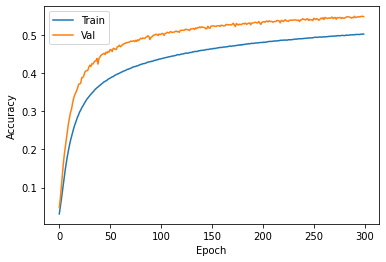
\includegraphics[width=\textwidth]{../Figures/accuracy_model}
    \caption{Model Categorical Accuracy.}
    \label{Fig:Model_Cat_Acc}
  \end{minipage}
  \hfill
  \begin{minipage}[b]{0.45\textwidth}
    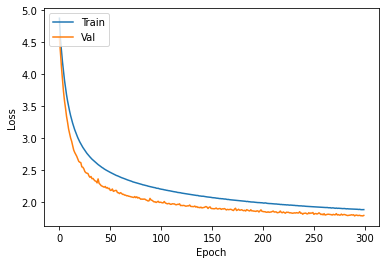
\includegraphics[width=\textwidth]{../Figures/loss_model}
    \caption{Model Loss.}
    \label{Fig:Model_Loss}
  \end{minipage}
\end{figure}

Figures \ref{Fig:Model_Cat_Acc} and \ref{Fig:Model_Loss} show the learning curves for the chosen hybrid model as a function of the training time measured in terms of the number of iterations. The categorical accuracy of the model is a percentage that measures how accurate were the predictions of the model, compared to the validation data (Figure \ref{Fig:Model_Cat_Acc}).  

The loss is calculated on training and validation and is used to evaluate how well the model performs for these two sets (Figure \ref{Fig:Model_Loss}). Unlike accuracy, a loss is not a percentage. Instead, it is a sum of the errors made for each example in training or validation sets.

According to both figures, the hybrid model makes it possible to recognize the temporal structure in a time series and predict their class with fair accuracy. The convergence of the loss between training and validation is also indicative that the model's performance is acceptable \cite{Charniak2019}. However, we see that the final loss value is relatively large. It indicates that the model could be further improved if we consider more training samples (which are not available for the dataset used in our case study).

\section{Spatio-Temporal Predictive Query Processing}
\label{Sec:SpatioTemporalPredictiveQuery}

After having implemented and evaluated the offline procedure, we now can process a spatio-temporal predictive query, which is denoted by the tuple (Section \ref{Sec:ProblemFormalization}):

\begin{equation*} 
Q = \langle R, t_{p}, t_{f}, Q_{m} \rangle,
\end{equation*}
where:
\begin{itemize}[noitemsep,nolistsep]	
	\item $R$: represents the size/shape/type of interest region,
	\item $t_{p}$: $\{s_{t-t_p}, s_{t-t_{p}+1}\ldots, s_{t}\}$ number of steps used for  prediction,
	\item $t_{f}$: $\{s_{t+1}, \ldots, s_{t+t_f}\}$ number of steps to predict ($n\geq 1$),
	\item $Q_{m}$: represents users qualitative measurements to evaluate the predictive output.
	%\item $Y_{Q}$: prediction output.
\end{itemize}

This section shows the experiments and results for the online procedure implemented to execute a spatio-temporal predictive query (Section \ref{Sec:SpatioTemporalQueryProcessing}). In Section \ref{Sec:ModelCompositionAggregated}, we used queries with regions of fixed size to evaluate the forecast error of different model compositions. Here, we will extend those results to include the classifier for predictive models discussed in the previous section and include $k$NN as a baseline for comparing the performance of ARIMA as a predictive model.

\subsection{Evaluating Spatio-Temporal Predictive Queries}
\label{Sec:ExperimentsQueries}

The process to evaluate a spatio-temporal predictive query is composed of four steps: i) receive a query, ii) data validation, iii) perform model composition; and iv) retrieve query result. The previous section consider the implementation of a classifier for the model composition process, an updated version of the prediction query process is represented in Figure \ref{Fig:OnLineQP_Update} The data validation consists of extracting elements from the domain corresponding to the query region with the $t_p$ instances. We denote this as $[R \times t_{p}]$. Next, the model composition computes the MSE of the forecast for the $t_{f}$ future values over the region of interest $R$. The output of the query has the forecast and a numeric value representing the MSE of the forecast error (we use the approach in \ref{sec:InSampleForecastErrors} to calculate the error for each element). 

\begin{figure}[h]
	\centering
	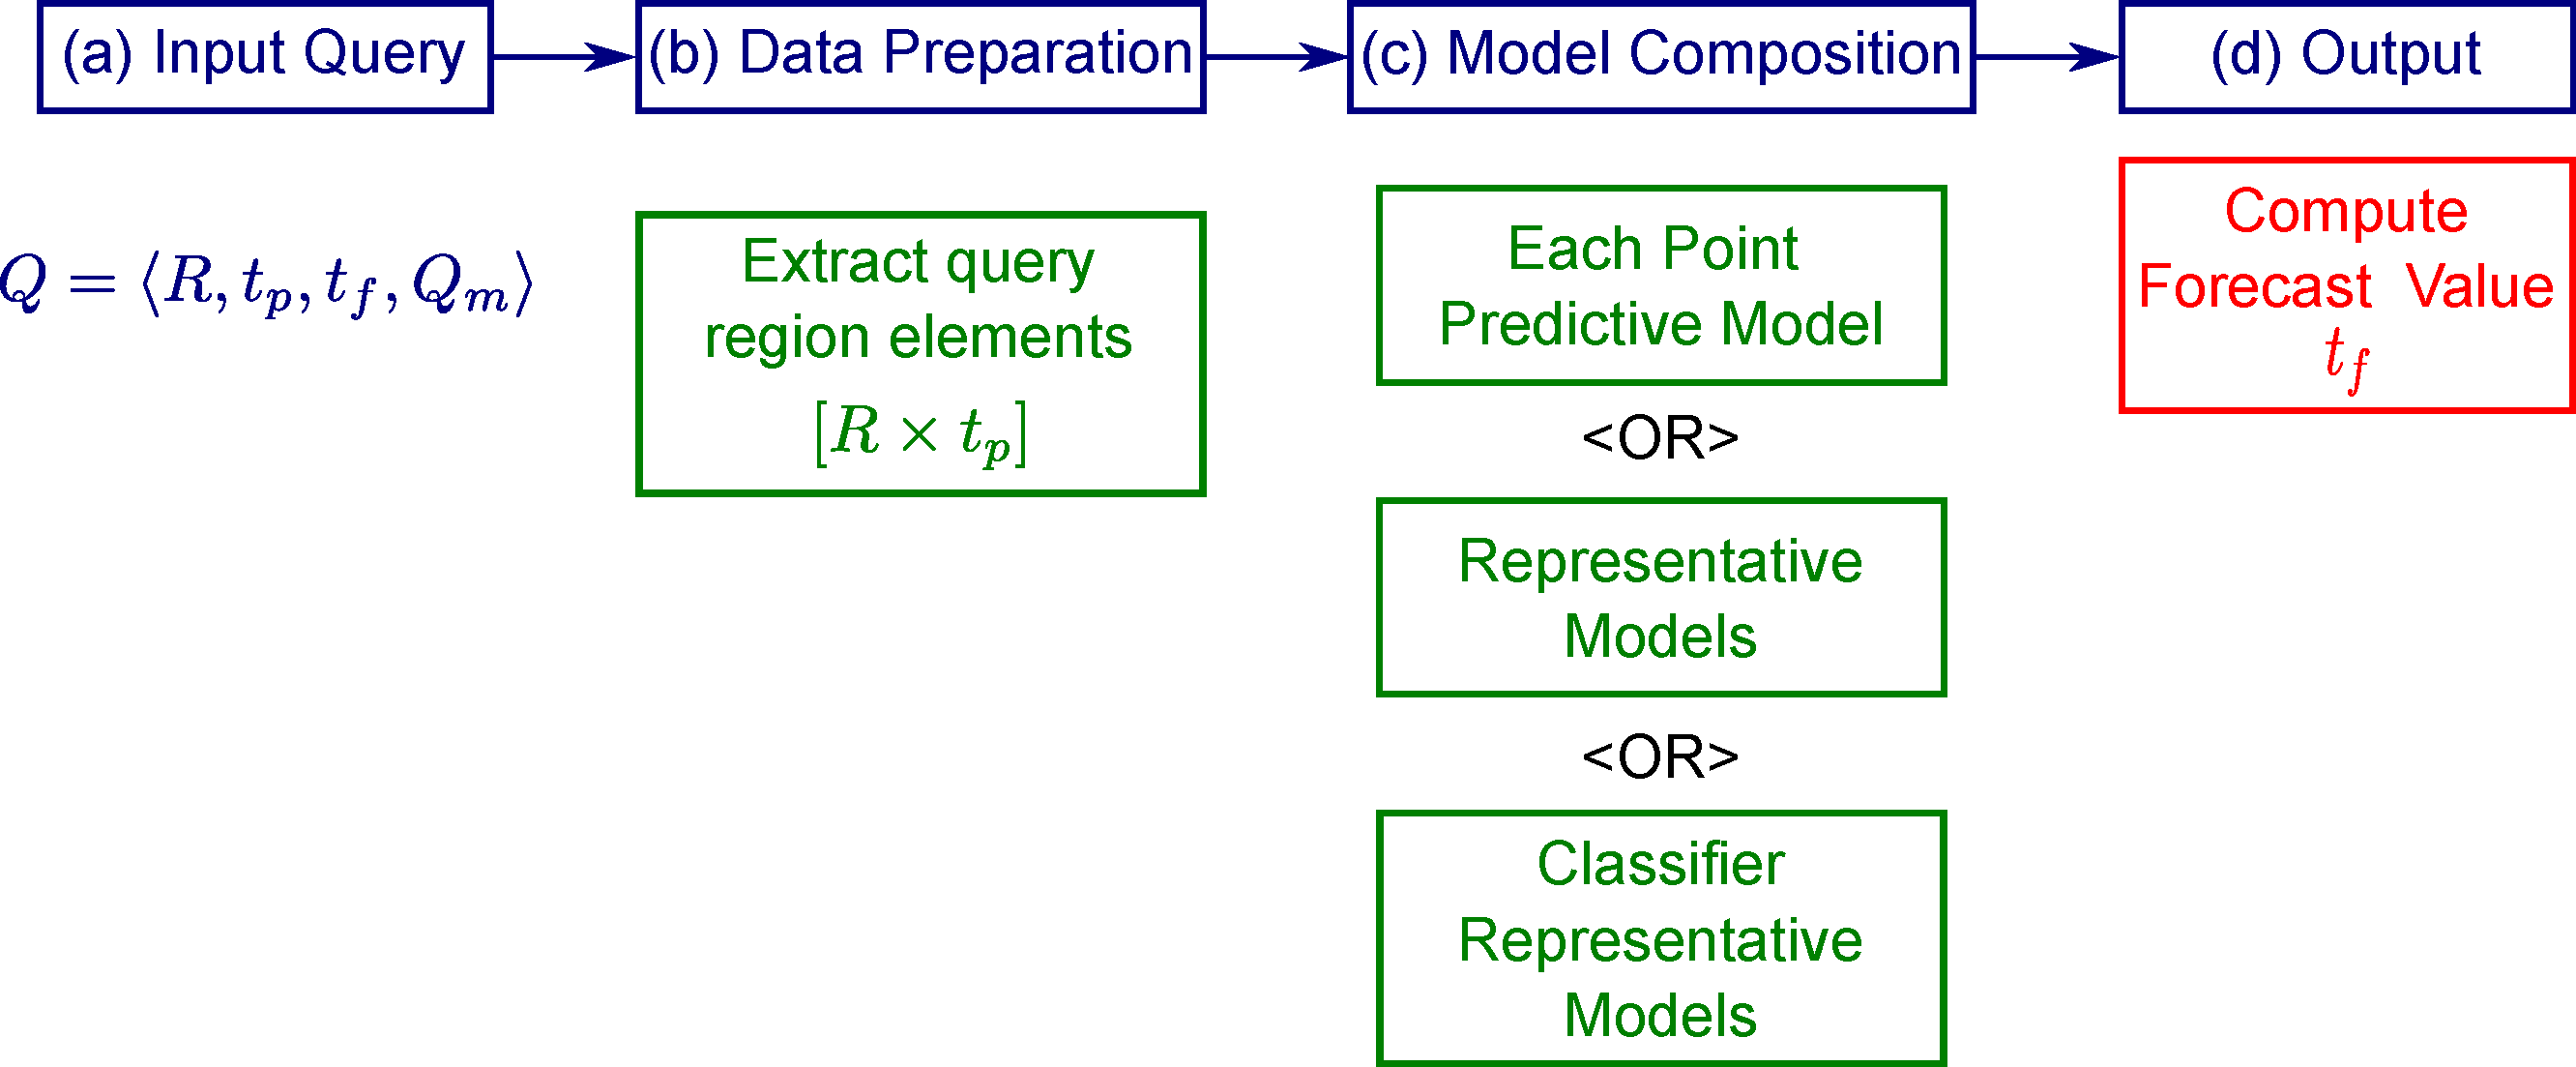
\includegraphics[scale=0.35]{../Figures/Query_Processing}
	\caption{Updated On-Line Processing Spatio-Temporal Predictive Query}
	\label{Fig:OnLineQP_Update}
\end{figure}

As previously established in Section \ref{Sec:SpatioTemporalQueryProcessing}, we elaborate experiments for the following model compositions:

\begin{itemize}
	\item Model Composition with Point Predictive Model: this is the naive approach, in which we train an ARIMA model on each element. Here, we introduce $k$NN as an additional predictive model for comparisons of forecast accuracy, so we obtain two sets of experimental results.
	\item Model Composition of Representative Predictive Models: for each element, we identify their respective representatives for the $k$-Medoids domain partitioning technique and use the model trained at the corresponding medoid to predict each element in the query region. We continue to consider the three partitioning schemes corresponding to $k=(8, 66, 132)$ like previous experiments.
	\item Model Composition of Classifier for Predictive Models: The solver that calculates the result of a prediction query using the outcome of the time series classifier developed in Section \ref{Sec:TrainingClassifier}. The classifier (implemented in Section \ref{Sec:ExperimentsTrainingClassifier}) is a function that, given an input series of size $t_{p}$, a predetermined suite of partitioning sizes, and a region, returns one of the representatives from any of the partitioning sizes available in the suite. Once the representative is determined, we follow the procedure for the `Model Composition of Representative Predictive Models' described in Section \ref{Sec:KnowledgExtraction}, but limited to the subset region $R$. As output, we obtain a representative label that corresponds with the predictive model used to make a forecast for the element.
	%It is the main model composition that we wish to evaluate, while the other two are presented for comparisons.
	%Model Composition of Classifier for Predictive Models: for each element in $R$ of size $t_{p}$, the classifier implemented in Section \ref{Sec:ExperimentsTrainingClassifier} receives the time series of length $t_{p}$ as input; as output, we obtain a representative label that corresponds with the predictive model used to make a forecast for the element.
\end{itemize}

In the same manner, the algorithm \ref{alg:modelcomp}, will consider the classifier as an option for the model composition process. The algorithm \ref{alg:modelcomp_update}, represents the process:

\begin{algorithm}[h!]
\caption{Load a Model Composition}\label{alg:modelcomp_update}
\begin{algorithmic}[1] 
\Function{load\_composition} {$D, comp\_id, t\_p$}

\State {$model\_comp\ \gets \bot$}

/* Model Composition with Point Predictive Models */
\If {$is\_point\_composition(comp\_id)$}

    
    /* Let model at each element predict its own element */
    \State{$model\_comp\ \gets load\_trained\_models\_each(D, t\_p)$}
    
\EndIf

/* Model Composition of Representative Predictive Models */
\If {$is\_representative\_composition(comp\_id)$}

    /* User needs to supply value for k of partitioning scheme */
    \State{$k\ \gets get\_k\_for\_request(comp\_id)$}
    
    /* Retrieve previously trained models at each representative */
    \State {$(medoids\_with\_models, D\_part)\ \leftarrow\ load\_models\_at\_medoids(D, k, t\_p)$}
    
    \For{$m \in medoids\_with\_models$}
    
        /* Retrieve the elements associated to current representative */
        \State {$cluster\ \gets elements\_represented\_by(m, D\_part)$}
        
        /* Let model at current representative predict these elements */
        \State{$model\_comp\ \gets set\_predictor(cluster, m, model\_comp)$}
    \EndFor

\EndIf

\If {$is\_classifier\_composition(comp\_id)$}

    /* Retrieve previously trained classifier */
    \State{$classifier\ \gets load\_trained\_classifier(comp\_id, t\_p)$}
    
    /* Classifier uses multiple partitioning schemes */
    \For{$k \in classifier.k\_list$}
    
        /* Retrieve previously trained models at each representative of current k */
        \State {$(medoids\_with\_models, D\_part)\ \leftarrow\ load\_models\_at\_medoids(D, k, t\_p)$}

        \For{$m \in medoids\_with\_models$}
        
            /* Determine label associated to current representative */
            \State {$medoid\_label\ \gets label\_for\_medoid(k, m, classifier)$}
            
            /* Let model at current representative predict elements that match label */
            \State{$model\_comp\ \gets assign\_predictor(medoid\_label, m, model\_comp)$}
        \EndFor

    \EndFor
\EndIf

\State {$Return \ model\_comp$}
\EndFunction 
\end{algorithmic} 
\end{algorithm}

To evaluate the performance of the model compositions above, we consider a forecast with $t_{f} = 8$. It allows us to compute the forecast error because we have the actual values in the dataset (also considered in Section \ref{Sec:AnalyzeForecastErrors}). 

In Section \ref{Sec:ModelCompositionAggregated}, we evaluate the predictive quality of the `Model Composition of Representative Predictive Models' for regions of size $10 \times 10$ distributed uniformly over the domain. Here, we complement the evaluation of our approach by adding the results obtained by the `Model Composition of Classifier for Predictive Models' and the results with the $k$NN baseline predictive model. The experimental results are summarized in Table \ref{Table:Query10x10_Classfier_Point_Each_StatSummary}: the first two result columns correspond to the first model composition with the two models; the next three columns represent the second model composition with the three values of $k$; the last column (highlighted) represents the third model composition using the classifier.

\begin{table}[h!]
	\centering
	\tiny
	\begin{tabular}{|c|c|c|c|c|c|c|}
	    \hline
        \multirow{2}{*}{Model Composition} & \multirow{2}{*}{ARIMA} & \multirow{2}{*}{$k$NN} & \multicolumn{3}{c|}{$k$-Medoids} & \multirow{2}{*}{Classifier}  \\
        \cline{4-6}
        & & & $k = 8$ & $k = 66$ & $k = 132$ &  \\
        %\cline{2-4}
        \hline
        Forecast Error ($t_{f}=8$) & $0.38 \pm 0.61$ & $0.62 \pm 0.91$ & $0.48 \pm 0.59$ & $0.47 \pm 0.86$ & $0.39 \pm 0.62$ & \cellcolor{red!20}$0.70 \pm 0.81$ \\
        \hline
	\end{tabular}
	\caption{Forecast Error Summary.}
	\label{Table:Query10x10_Classfier_Point_Each_StatSummary}
\end{table}

To aid in visualizing these results, we show colormaps for the variation of the forecast errors computed in different regions of the domain in Figures \ref{Fig:model_composition_classifier} and \ref{Fig:model_composition_each}. Each colormap shows the relative intensity of values captured: we assign a dark blue to the highest forecast error, while those lower in their value will be given a lighter blue. The color palette has been kept constant for both figures for visual comparisons.

\begin{figure}[!tbp]
  \centering
    \begin{minipage}[b]{0.45\textwidth}
    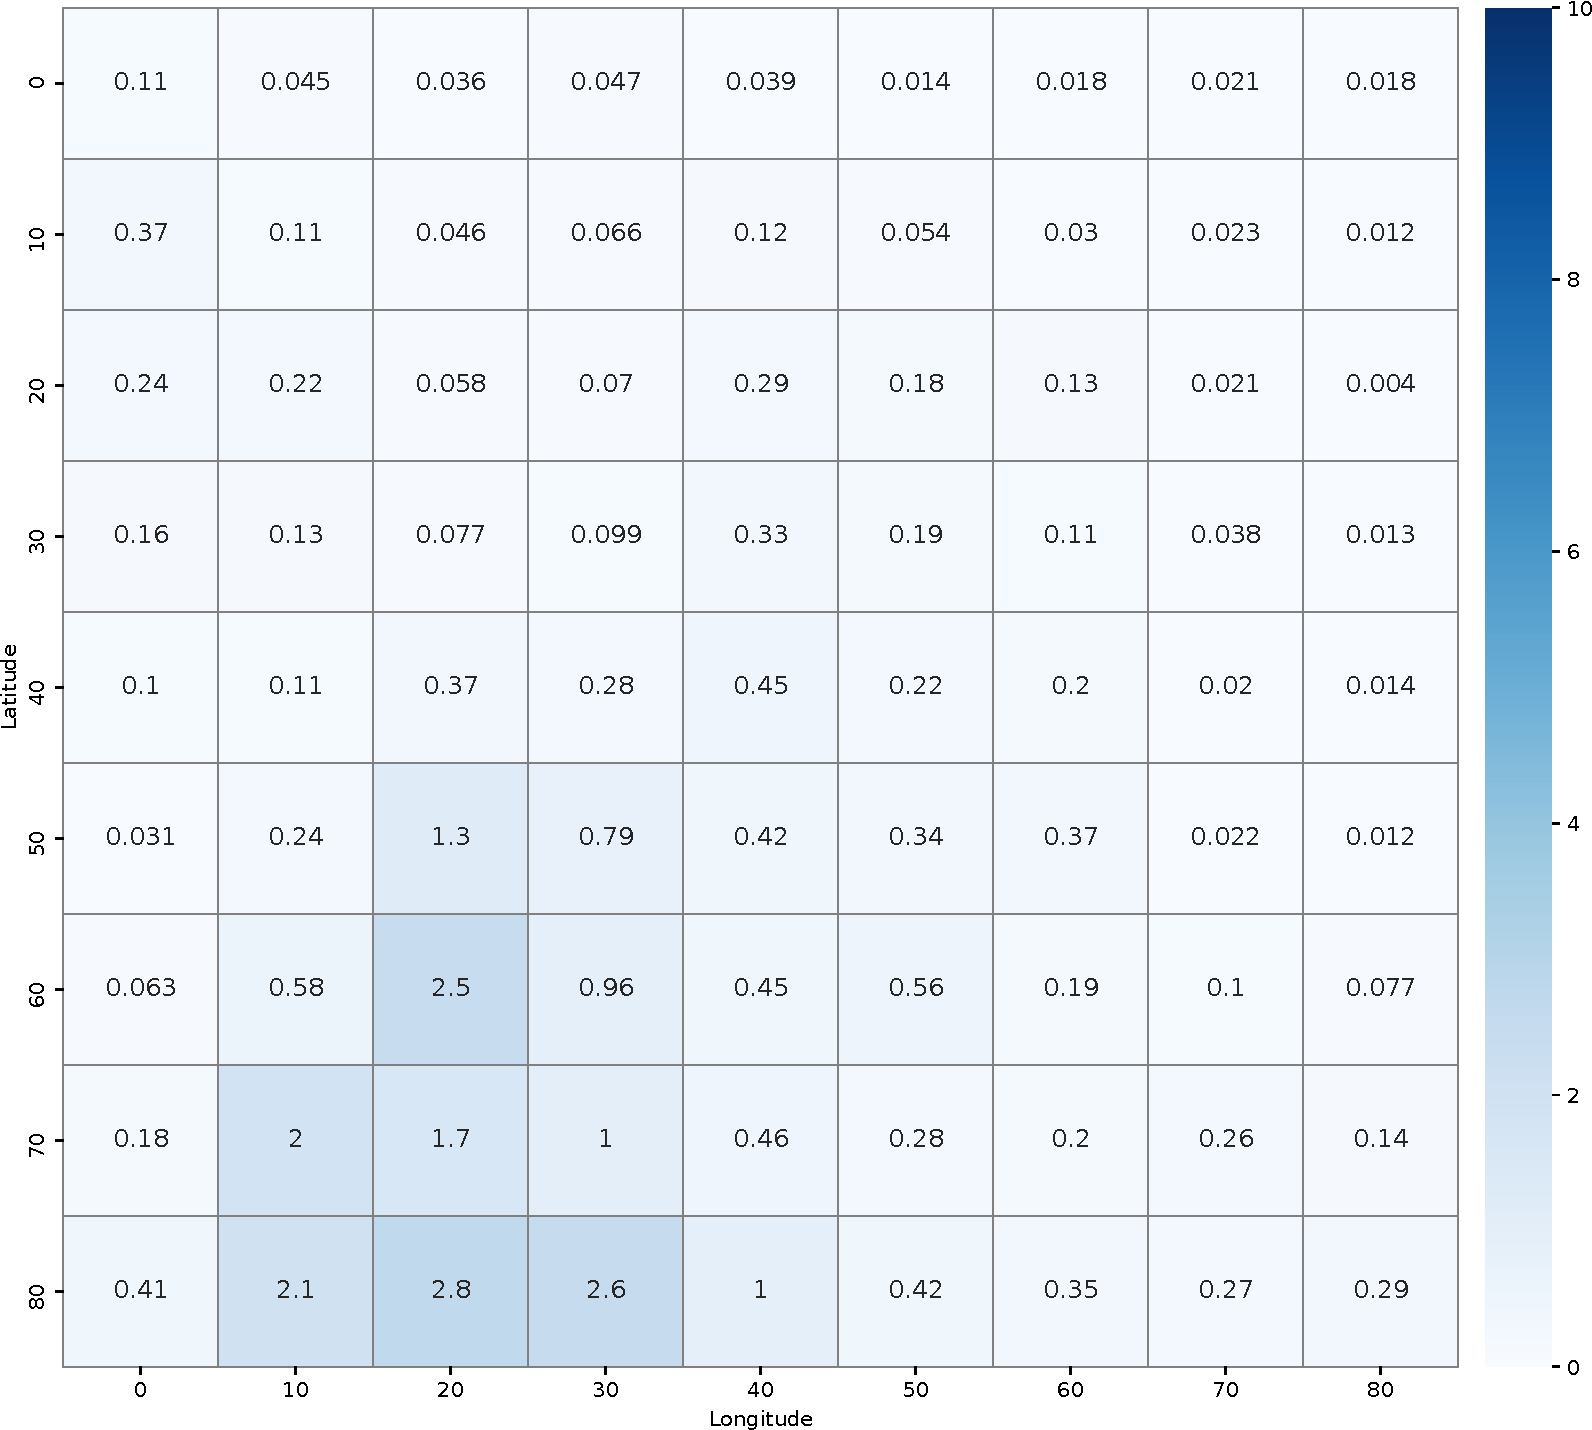
\includegraphics[width=\textwidth]{../Figures/query_10x10_solver-each-1000dpi}
    \caption{Forecast Error with ARIMA Model at Each Element.}
    \label{Fig:model_composition_each}
  \end{minipage}
  \hfill
    \begin{minipage}[b]{0.45\textwidth}
    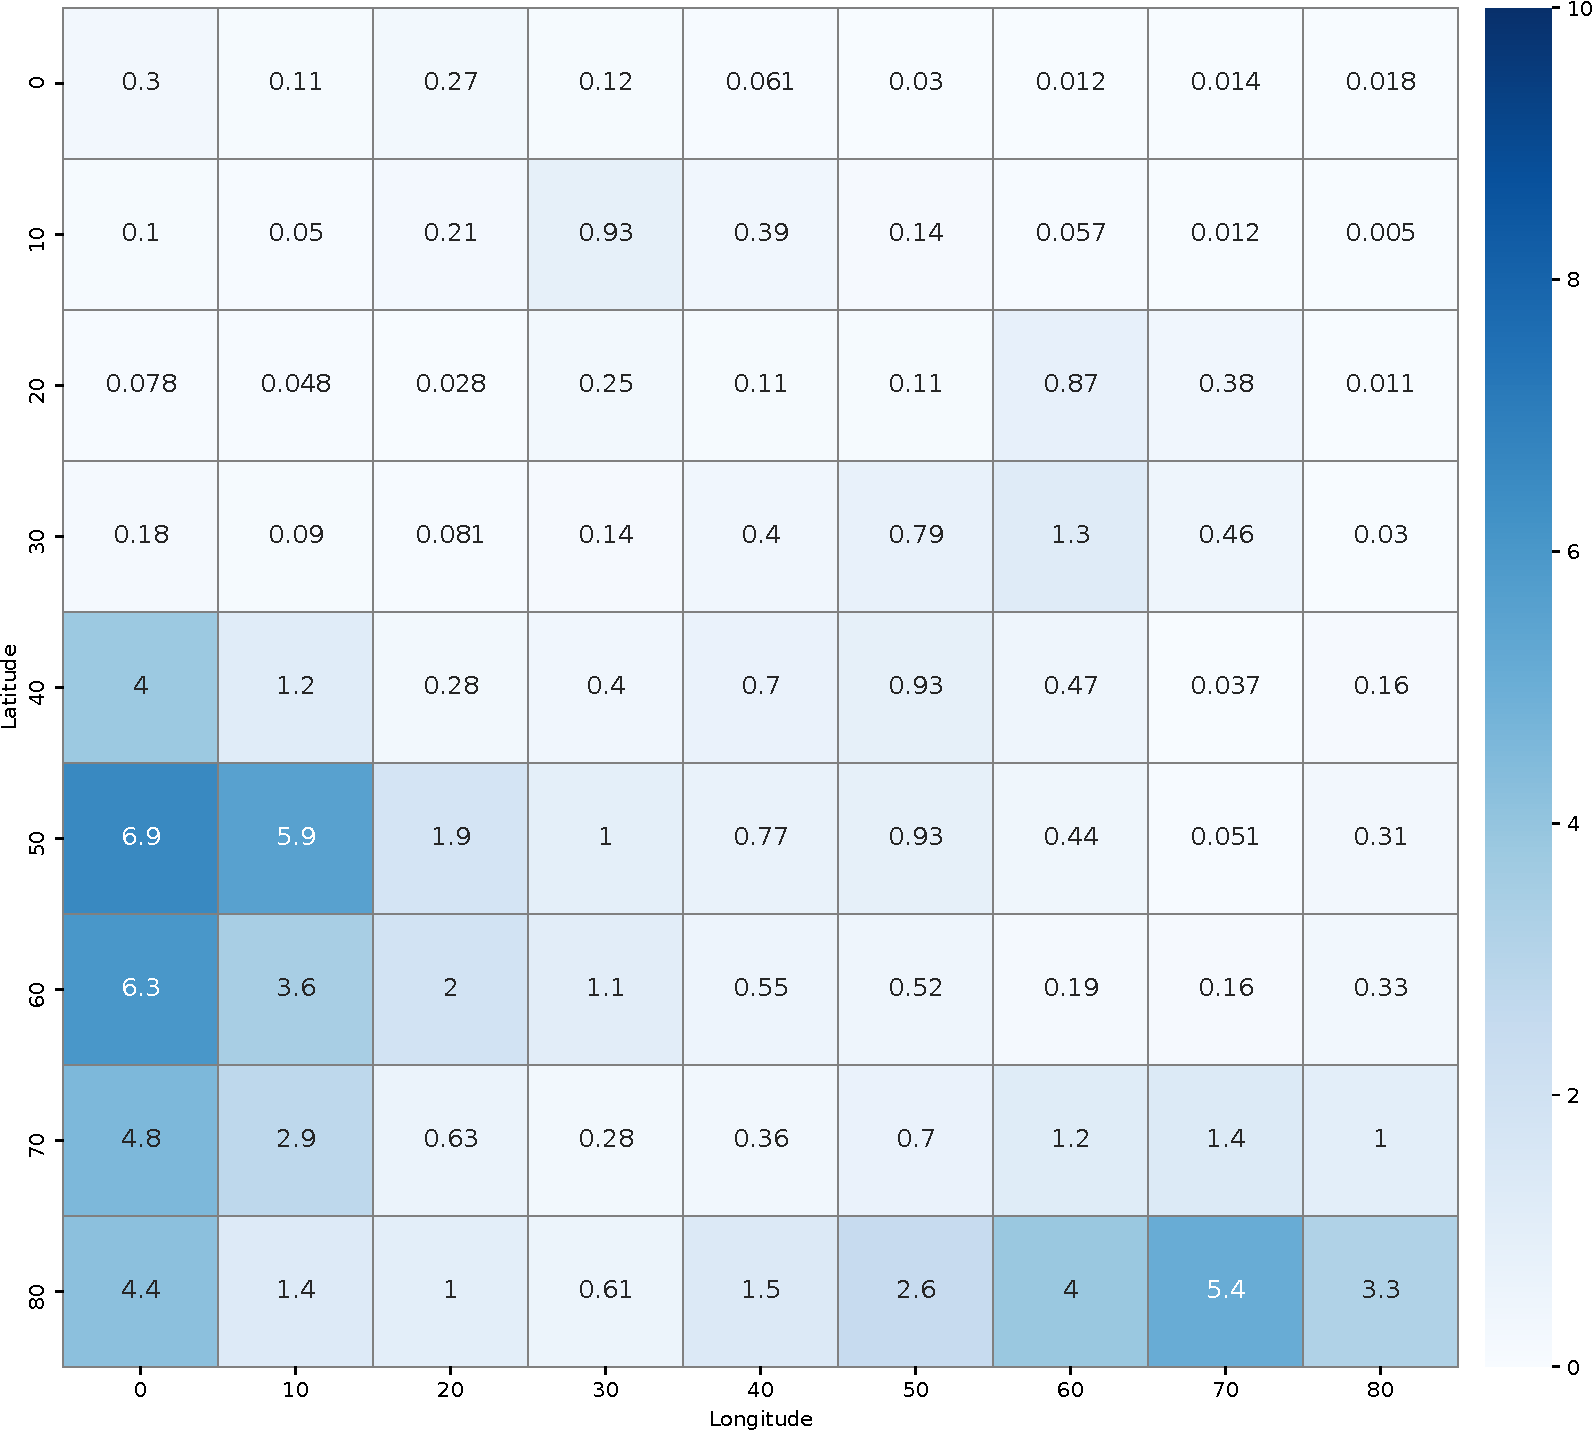
\includegraphics[width=\textwidth]{../Figures/query_10x10_solver-multiclass-1000dpi}
    \caption{Forecast Error with Model Composition by Classifier.}
    \label{Fig:model_composition_classifier}
  \end{minipage}
\end{figure}

The forecast error obtained using the proposed methodology, supported by a time-series classifier, presents variations for different regions in the domain. In some areas, the classifier generates a composition comparable with the naive approach, while the predictive performance is poorer for others. One of the reasons is that the predictive quality of the classifier (See Section \ref{Sec:TSC_NN_Results} for its evaluation) is reasonably good. However, we show that it is possible to improve. We observe that the quality of the classifier is reflected in a few regions of the domain that exhibit a higher forecast error than when using the corresponding representative directly.

Additionally, we consider queries in different regions with variable sizes. The results obtained for these queries are summarized in Table \ref{Table:MSEForecasError}, which follows a similar structure as the previous table. Again we can observe the previous tendency of the classifier to produce acceptable results for most areas of the domain.

\begin{table}[h]	
    \centering
	\small
	\begin{tabular}{|c|c|r|r|r|r|r|r|}
        \hline
        \multirow{3}{*}{Size} & \multirow{3}{*}{Query Region} & \multicolumn{6}{c|}{Model Composition} \\ 
        \cline{3-8}
        & & \multirow{2}{*}{ARIMA} & \multirow{2}{*}{$k$NN} & \multicolumn{3}{c|}{$k$--Medoids} & \multirow{2}{*}{Classifier} \\ 
        \cline{5-7}
        & & & & $k =8$ & $k = 66$ & $k = 132$ &  \\ \hline % & DJEnsemble \\ \hline
        $20 \times 20$ & $[ 0, 20] \times [ 0, 20]$ & 0.158 & 0.209 & 0.089 & 0.174 & 0.160 & \cellcolor{red!20}0.190  \\ % &  935.748\\ %30.590 \\
        $20 \times 20$ & $[20, 40] \times [35, 55]$ & 0.203 & 0.258 & 0.335 & 0.199 & 0.230 & \cellcolor{red!20}0.330 \\ % &  993.826\\ %31.525 \\
        $20 \times 20$ & $[50, 70] \times [60, 80]$ & 0.170 & 0.145 & 0.584 & 0.203 & 0.188 & \cellcolor{red!20}0.274 \\ % & 6572.021\\ %81.068 \\
        $20 \times 20$ & $[15, 35] \times [65, 85]$ & 0.034 & 0.067 & 0.063 & 0.045 & 0.038 & \cellcolor{red!20}0.093 \\ % & 4641.424\\%68.128 \\
        $30 \times 30$ & $[20, 50] \times [50, 80]$ & 0.122 & 0.210 & 0.203 & 0.147 & 0.135 & \cellcolor{red!20}0.202 \\ % & 1410.378\\%37.555 \\
        $30 \times 30$ & $[15, 45] \times [20, 50]$ & 0.156 & 0.198 & 0.262 & 0.155 & 0.168 & \cellcolor{red!20}0.281 \\ %  & 1205.687\\%34.723 \\
        $15 \times 20$ & $[40, 55] \times [20, 40]$ & 0.483 & 0.707 & 0.707 & 0.530 & 0.541 & \cellcolor{red!20}0.618 \\ % &  905.829\\%30.097 \\
        $15 \times 20$ & $[65, 80] \times [50, 70]$ & 0.248 & 0.190 & 0.470 & 0.302 & 0.308 & \cellcolor{red!20}0.343 \\ %& 6382.732\\%79.892 \\
        $30 \times 15$ & $[30, 60] \times [ 5, 20]$ & 0.137 & 0.208 & 0.353 & 0.205 & 0.147 & \cellcolor{red!20}0.391 \\ % &  950.797\\%30.835 \\
        $30 \times 15$ & $[10, 40] \times [55, 70]$ & 0.095 & 0.226 & 0.139 & 0.111 & 0.098 & \cellcolor{red!20}0.135 \\ %& 4546.940\\ \hline% 67.431 \\ 
        \hline
	\end{tabular}
	\caption{MSE Forecast Error for Spatio-Temporal Queries in the domain $\mathcal{D}$.}
	\label{Table:MSEForecasError}
\end{table}

Furthermore, we compare the execution of a spatio--temporal predictive query with the model composition formed by our approach, with the naive approaches based on ARIMA and $k$NN regressions for univariate time series. It is possible to observe that, for the majority of the query regions considered, the forecast error obtained with the proposed classifier is closer to the ARIMA naive approach than to the $k$NN, and we can confidently conclude that the classifier performs better than the baseline approach based on $k$NN.

\section{Summary} 

This chapter presented the experiments and results obtained to evaluate our methodology using temperature forecast. As a general summary, our approach presents acceptable predictive performance for the execution of spatio-temporal predictive queries, when compared to the naive approach where a predictive model is trained for each element of the domain and used for forecasting. %with data with correlation between data and time. The results could be improved by considering a domain with more volume of data. We  describe  performance  analyses to compare and evaluate forecasting procedures

The extensive experiments for the analysis of the domain partitioning techniques point towards $k$--Medoids being the superior choice against the baseline approach of a naive partitioning based on geometry, specifically regarding the intra-cluster costs. While we could have included other comparisons such as using the Euclidian distance, the results obtained during the forecast analysis already show that $k$--Medoids produced satisfactory results. Moreover, using the Euclidean distance also represents a significant computational effort given the size of the dataset. In this context, the creation of the DTW matrix as an offline and parallelizable process proved to be very beneficial in terms of computational resources required, as we showed that the volume of experiments would have been unfeasible without the matrix.

Regarding the forecast analysis, our experiments indicate that the chosen model composition based on $k$--Medoids representatives can provide a predictive performance that is closer to the ideal scenario where we always use a model representative that provides the minimum possible forecast error for the group. While we accept that the predictive performance is inferior to the naive scenario, we argue that this loss in accuracy is completely justified by the very significant performance gains obtained, and this can prove to be useful in many areas where a predictive system with a faster service time is deemed more valuable than a slightly more accurate system.

The results from the forecast analysis further support the use of a time-series classifier to try and leverage the potential gains in predictive performance when using multiple partitioning schemes. However, we recognize that the results obtained for the case study considered could be improved by considering a domain with a larger volume of data, and this was demonstrated using performance metrics from the training of the classifier.

Finally, we believe that the way of presenting results from the forecast analysis using colormaps is very convenient in understanding the performance of the models at a glance, and helped identify problematic regions where the loss of accuracy is more pronounced. This approach could also be leveraged to apply a different, more refined approach in those areas.